% Options for packages loaded elsewhere
\PassOptionsToPackage{unicode}{hyperref}
\PassOptionsToPackage{hyphens}{url}
%
\documentclass[
  letterpaper,
  openany]{book}
\usepackage{amsmath,amssymb}
\usepackage{lmodern}
\usepackage{setspace}
\usepackage{ifxetex,ifluatex}
\ifnum 0\ifxetex 1\fi\ifluatex 1\fi=0 % if pdftex
  \usepackage[T1]{fontenc}
  \usepackage[utf8]{inputenc}
  \usepackage{textcomp} % provide euro and other symbols
\else % if luatex or xetex
  \usepackage{unicode-math}
  \defaultfontfeatures{Scale=MatchLowercase}
  \defaultfontfeatures[\rmfamily]{Ligatures=TeX,Scale=1}
  \setmainfont[]{Roboto}
  \setmathfont[]{Fira Math Regular}
\fi
% Use upquote if available, for straight quotes in verbatim environments
\IfFileExists{upquote.sty}{\usepackage{upquote}}{}
\IfFileExists{microtype.sty}{% use microtype if available
  \usepackage[]{microtype}
  \UseMicrotypeSet[protrusion]{basicmath} % disable protrusion for tt fonts
}{}
\makeatletter
\@ifundefined{KOMAClassName}{% if non-KOMA class
  \IfFileExists{parskip.sty}{%
    \usepackage{parskip}
  }{% else
    \setlength{\parindent}{0pt}
    \setlength{\parskip}{6pt plus 2pt minus 1pt}}
}{% if KOMA class
  \KOMAoptions{parskip=half}}
\makeatother
\usepackage{xcolor}
\IfFileExists{xurl.sty}{\usepackage{xurl}}{} % add URL line breaks if available
\IfFileExists{bookmark.sty}{\usepackage{bookmark}}{\usepackage{hyperref}}
\hypersetup{
  pdftitle={Evan's PhD thesis proposal},
  pdfauthor={Evan C Mascitti},
  hidelinks,
  pdfcreator={LaTeX via pandoc}}
\urlstyle{same} % disable monospaced font for URLs
\usepackage[left=1.5in, right=1.5in, top=1in, bottom=1in]{geometry}
\usepackage{color}
\usepackage{fancyvrb}
\newcommand{\VerbBar}{|}
\newcommand{\VERB}{\Verb[commandchars=\\\{\}]}
\DefineVerbatimEnvironment{Highlighting}{Verbatim}{commandchars=\\\{\}}
% Add ',fontsize=\small' for more characters per line
\usepackage{framed}
\definecolor{shadecolor}{RGB}{248,248,248}
\newenvironment{Shaded}{\begin{snugshade}}{\end{snugshade}}
\newcommand{\AlertTok}[1]{\textcolor[rgb]{0.94,0.16,0.16}{#1}}
\newcommand{\AnnotationTok}[1]{\textcolor[rgb]{0.56,0.35,0.01}{\textbf{\textit{#1}}}}
\newcommand{\AttributeTok}[1]{\textcolor[rgb]{0.77,0.63,0.00}{#1}}
\newcommand{\BaseNTok}[1]{\textcolor[rgb]{0.00,0.00,0.81}{#1}}
\newcommand{\BuiltInTok}[1]{#1}
\newcommand{\CharTok}[1]{\textcolor[rgb]{0.31,0.60,0.02}{#1}}
\newcommand{\CommentTok}[1]{\textcolor[rgb]{0.56,0.35,0.01}{\textit{#1}}}
\newcommand{\CommentVarTok}[1]{\textcolor[rgb]{0.56,0.35,0.01}{\textbf{\textit{#1}}}}
\newcommand{\ConstantTok}[1]{\textcolor[rgb]{0.00,0.00,0.00}{#1}}
\newcommand{\ControlFlowTok}[1]{\textcolor[rgb]{0.13,0.29,0.53}{\textbf{#1}}}
\newcommand{\DataTypeTok}[1]{\textcolor[rgb]{0.13,0.29,0.53}{#1}}
\newcommand{\DecValTok}[1]{\textcolor[rgb]{0.00,0.00,0.81}{#1}}
\newcommand{\DocumentationTok}[1]{\textcolor[rgb]{0.56,0.35,0.01}{\textbf{\textit{#1}}}}
\newcommand{\ErrorTok}[1]{\textcolor[rgb]{0.64,0.00,0.00}{\textbf{#1}}}
\newcommand{\ExtensionTok}[1]{#1}
\newcommand{\FloatTok}[1]{\textcolor[rgb]{0.00,0.00,0.81}{#1}}
\newcommand{\FunctionTok}[1]{\textcolor[rgb]{0.00,0.00,0.00}{#1}}
\newcommand{\ImportTok}[1]{#1}
\newcommand{\InformationTok}[1]{\textcolor[rgb]{0.56,0.35,0.01}{\textbf{\textit{#1}}}}
\newcommand{\KeywordTok}[1]{\textcolor[rgb]{0.13,0.29,0.53}{\textbf{#1}}}
\newcommand{\NormalTok}[1]{#1}
\newcommand{\OperatorTok}[1]{\textcolor[rgb]{0.81,0.36,0.00}{\textbf{#1}}}
\newcommand{\OtherTok}[1]{\textcolor[rgb]{0.56,0.35,0.01}{#1}}
\newcommand{\PreprocessorTok}[1]{\textcolor[rgb]{0.56,0.35,0.01}{\textit{#1}}}
\newcommand{\RegionMarkerTok}[1]{#1}
\newcommand{\SpecialCharTok}[1]{\textcolor[rgb]{0.00,0.00,0.00}{#1}}
\newcommand{\SpecialStringTok}[1]{\textcolor[rgb]{0.31,0.60,0.02}{#1}}
\newcommand{\StringTok}[1]{\textcolor[rgb]{0.31,0.60,0.02}{#1}}
\newcommand{\VariableTok}[1]{\textcolor[rgb]{0.00,0.00,0.00}{#1}}
\newcommand{\VerbatimStringTok}[1]{\textcolor[rgb]{0.31,0.60,0.02}{#1}}
\newcommand{\WarningTok}[1]{\textcolor[rgb]{0.56,0.35,0.01}{\textbf{\textit{#1}}}}
\usepackage{longtable,booktabs,array}
\usepackage{calc} % for calculating minipage widths
% Correct order of tables after \paragraph or \subparagraph
\usepackage{etoolbox}
\makeatletter
\patchcmd\longtable{\par}{\if@noskipsec\mbox{}\fi\par}{}{}
\makeatother
% Allow footnotes in longtable head/foot
\IfFileExists{footnotehyper.sty}{\usepackage{footnotehyper}}{\usepackage{footnote}}
\makesavenoteenv{longtable}
\usepackage{graphicx}
\makeatletter
\def\maxwidth{\ifdim\Gin@nat@width>\linewidth\linewidth\else\Gin@nat@width\fi}
\def\maxheight{\ifdim\Gin@nat@height>\textheight\textheight\else\Gin@nat@height\fi}
\makeatother
% Scale images if necessary, so that they will not overflow the page
% margins by default, and it is still possible to overwrite the defaults
% using explicit options in \includegraphics[width, height, ...]{}
\setkeys{Gin}{width=\maxwidth,height=\maxheight,keepaspectratio}
% Set default figure placement to htbp
\makeatletter
\def\fps@figure{htbp}
\makeatother
\setlength{\emergencystretch}{3em} % prevent overfull lines
\providecommand{\tightlist}{%
  \setlength{\itemsep}{0pt}\setlength{\parskip}{0pt}}
\setcounter{secnumdepth}{5}
% a useful website for knowing what things are called in latex
% http://www.texfaq.org/FAQ-fixnam



% packages I had already put in here 
\usepackage[none]{hyphenat}
\usepackage[font=small,labelfont=bf]{caption}


% all packages that kableExtra depends on 
\usepackage{booktabs}
\usepackage{longtable}
\usepackage{array}
\usepackage{multirow}
\usepackage{wrapfig}
\usepackage{float}
\usepackage{colortbl}
\usepackage{pdflscape}
\usepackage{tabu}
\usepackage{threeparttable}
\usepackage{threeparttablex}
\usepackage[normalem]{ulem}
% this one not needed because I always use UTF-8 \usepackage[utf8]{inputenc}
\usepackage{makecell}
\usepackage{xcolor}

%%%%%%%%%%%%%%%%%%%%%%%%%%%%%%%%%%%%%%%%%%%%%%%%%%%%%%%%%%%%%
% load cancel package for clearer unit conversions
\usepackage{cancel}
%%%%%%%%%%%%%%%%%%%%%%%%%%%%%%%%%%%%%%%%%%%%%%%%%%%%%%%%%%%%%

% apparently this package makes better bookmarks, 
% I need it for putting the TOC into the document tree
% see https://tex.stackexchange.com/questions/65544/how-to-link-table-of-contents-in-thesis-pdf

\usepackage{bookmark}



%%%%%%%%%%%%%%%%%%%%%%%%%%%%%%%%%%%%%%%%%%%%%%%%%%%%%%%%%%%%%


% set vertical line spacing for amsmath equations 
\setlength{\jot}{8pt}

% everything abve works well

% extras that I am testing come below 


% set paragraph indentation back to > 0; default is 20pt
\parindent=10pt



% define navy as a link color and use it for internal links
% depends on xcolor which is already loaded above 
\definecolor{dodgerblue4}{HTML}{104E8B}
\usepackage{hyperref}

\hypersetup{
  colorlinks=true,
  urlcolor=blue,
  linkcolor=dodgerblue4
}


% \linkcolor{navy}


% number the lines with small grey text, see https://tex.stackexchange.com/questions/247165/can-i-change-linenumber-colour
\usepackage{lineno}

% define R's grey90 color in HTML hex notation
\definecolor{grey90}{HTML}{E5E5E5}

% set color of line numbers 
% this was the code I copied from the URL above \renewcommand{\linenumberfont}{\normalfont\bfseries\small\color{grey75}}

% and this is my own version which uses the mono font. 
% To turn off, comment out the following line and also the line right after the table of contents that turns the line numbers on. 
\renewcommand{\linenumberfont}{\ttfamily\small\color{grey90}}




% Use the section numbers instead of titles because some of 
% my sections are spilling off the page 

% \usepackage{fancyhdr}
% \pagestyle{fancy}
% 
% \renewcommand{\sectionmark}
% {\thesection}

% this is what I _really_ want: truncate the header 
% only when it is too long, and add an ellipsis
% see https://tex.stackexchange.com/questions/6862/how-can-i-display-a-short-chapter-name-in-the-header-and-a-long-chapter-name-in/6866

 % \usepackage[fit]{truncate}
 % \usepackage{fancyhdr}
 % \pagestyle{fancy}
 % \fancyhead[RO,LE]{\truncate{.95\headwidth}{\leftmark}}
 
 \usepackage{fancyhdr}
 \fancyhead[LE,RO]{\thechapter}
 
 %%%%%%%%%%%%%%%%%%%%
 
 
 % limit depth of numbered sections and table of contents 
\setcounter{secnumdepth}{3}
\setcounter{tocdepth}{1} % chapter level is 0
 
 %%%%%%%%%%%%%%%%%%%%
% this one works if all else fails....not using any add-on packages;
% see https://latexref.xyz/_005cchapter.html

\renewcommand{\chaptername}{Section}


% A simple version to just change the chapter label and format 
% see the docs, it is a shortcut instead of specifying the 
% entire formatting command. But it seems to do what I want

% I figured this out on my own (i.e. no hyperlink - see Section 2.4, "quick reference"
% in the docs for titlesec, link is http://mirrors.ctan.org/macros/latex/contrib/titlesec/titlesec.pdf

% \usepackage{titlesec}
% \titlelabel{Section \thechapter \quad}


%%%%%%%%%%%%%%%%%%%%%%%%%%%%%%%%%%%

% a more complex example using the titlesec package from overleaf
% see https://www.overleaf.com/learn/latex/sections_and_chapters#Document_chapters_and_sections_in_a_Book.2FReport


% A more complex example from the  titles package
% I changed the font size to Huge instead of Large but it doesn't seem to change 
% much. But I have to leave this alone for now and get back to something more 
% pressing 

% \usepackage{titlesec}
% 
% \titleformat
% {\chapter} % command
% [display] % shape
% {\bfseries\Huge\itshape} % format
% {Section \ \thechapter} % label
% {0.5ex} % sep
% {
%     \rule{\textwidth}{1pt}
%     \vspace{1ex}
%     \centering
% } % before-code
% [
% \vspace{-0.5ex}%
% \rule{\textwidth}{0.3pt}
% ] % after-code

%%%%%%%%%%%%%%%%%%%%%%%%%%%%%%%%%%%%


% re-style block quotations??
% there are 2 environments that handle block quotations- the quotation environment 
% is for multi-paragraph quotes and each paragraph is indented.
% the quote environment is meant for shorter quotes. Evidently R Markdown 
% puts at least the short ones in the quote environment; I discovered this by 
% inspecting the .tex file usingkeep_tex: true in the YAML


% see https://stackoverflow.com/questions/4018493/vertical-line-with-every-quotation/4023967
% for solution
\usepackage{framed}


% define R's grey30 color in HTML hex notation
\definecolor{grey30}{HTML}{4D4D4D}

% change bar size to 0.5 pt instead of the default 3 pt
% use the newly defined grey color 
\renewenvironment{leftbar}{\def\FrameCommand{\color{grey30}\vrule width 1pt \hspace{10pt}}\MakeFramed {\advance\hsize-\width \FrameRestore}}{\endMakeFramed}

% for multi-paragraph quotations 
% \renewenvironment{quotation}%
% {\begin{leftbar}\begin{quotation}}%
% {\end{quotation}\end{leftbar}}

% for single-paragraph quotations 
% remove indent with \noindent

% \usepackage{tgpagella} % loads the font packge needed for the quote font I will use, but it is over-riding my Arial font for _everything_ not just the quote environment
% see https://tex.stackexchange.com/questions/193736/changing-font-in-a-particular-environment/193740
% and https://www.overleaf.com/learn/latex/Font_typefaces for inspiration 

% I had this inside the environment, after the begin quotation statement 
% \fontfamily{qpl}\selectfont

\renewenvironment{quote}%
{\begin{leftbar} \begin{quotation} \noindent \small }%
{\end{quotation}\end{leftbar}}




% the following 2 lines place a border around all figures 
% \floatstyle{boxed} 
% \restylefloat{figure}

\usepackage{booktabs}
\usepackage{longtable}
\usepackage{array}
\usepackage{multirow}
\usepackage{wrapfig}
\usepackage{float}
\usepackage{colortbl}
\usepackage{pdflscape}
\usepackage{tabu}
\usepackage{threeparttable}
\usepackage{threeparttablex}
\usepackage[normalem]{ulem}
\usepackage{makecell}
\usepackage{xcolor}
\ifluatex
  \usepackage{selnolig}  % disable illegal ligatures
\fi
\newlength{\cslhangindent}
\setlength{\cslhangindent}{1.5em}
\newlength{\csllabelwidth}
\setlength{\csllabelwidth}{3em}
\newenvironment{CSLReferences}[2] % #1 hanging-ident, #2 entry spacing
 {% don't indent paragraphs
  \setlength{\parindent}{0pt}
  % turn on hanging indent if param 1 is 1
  \ifodd #1 \everypar{\setlength{\hangindent}{\cslhangindent}}\ignorespaces\fi
  % set entry spacing
  \ifnum #2 > 0
  \setlength{\parskip}{#2\baselineskip}
  \fi
 }%
 {}
\usepackage{calc}
\newcommand{\CSLBlock}[1]{#1\hfill\break}
\newcommand{\CSLLeftMargin}[1]{\parbox[t]{\csllabelwidth}{#1}}
\newcommand{\CSLRightInline}[1]{\parbox[t]{\linewidth - \csllabelwidth}{#1}\break}
\newcommand{\CSLIndent}[1]{\hspace{\cslhangindent}#1}

\title{Evan's PhD thesis proposal}
\author{Evan C Mascitti}
\date{\texttt{last\ compiled\ Mon.\ 2021-06-28,\ \ 9:11\ AM}}

\begin{document}
\maketitle

\setstretch{1.2}
\hypertarget{exeuctive-summary}{%
\chapter*{Executive summary}\label{exeuctive-summary}}
\addcontentsline{toc}{chapter}{Executive summary}

This document outlines the research progress I have made since beginning my PhD in 2019 and describes my plans for completing the project.
It comprises 4 main sections:

\begin{description}
\item[{Section \ref{purpose-and-objectives} \protect\hyperlink{purpose-and-objectives}{Purpose and objectives}}]
High-level overview of project goals.
\item[{Section \ref{problem-description} \protect\hyperlink{problem-description}{Problem description}}]
Outlines the importance of the infield skin.
\item[{Section \ref{lit-review} \protect\hyperlink{lit-review}{Review of literature}}]
Summary of relevant prior scientific research.
\item[{Section \ref{proposed-experiments} \protect\hyperlink{proposed-experiments}{Proposed experiments}}]
Details of my research plan.
\end{description}

I have also included a description of my workflow and data management practices (Section \ref{workflow}).
This section is written informally.
Although it is un-related to the technical/soils aspects of my project, I included it because it forms an important practical part of completing my degree.
Regardless of whether the reader finds this section enlightening, writing it has served as a useful ``statement of beliefs'' for me.

I briefly define some terms and symbols in Section \ref{definition-of-terms}.
The proposal concludes with a list of \protect\hyperlink{references}{references} and an \protect\hyperlink{appendix}{Appendix} housing additional tables and equations.

\pdfbookmark[chapter]{\contentsname}{toc}

\tableofcontents

\pdfbookmark[0]{List of Figures}{lof}

\listoffigures

\pdfbookmark[0]{List of Tables}{lot}

\listoftables

\linenumbers

\hypertarget{purpose-and-objectives}{%
\chapter{Purpose and Objectives}\label{purpose-and-objectives}}

\hypertarget{purpose}{%
\section{Purpose}\label{purpose}}

Baseball fields can be improved by using the scientific method.
A high-quality playing surface enhances the safety, enjoyment, and economic value of the game at all levels of play.
Potential beneficiaries include grounds managers, soil suppliers, contractors, professional franchises, recreation associations, and the athletes themselves.

\hypertarget{objectives}{%
\section{Objectives}\label{objectives}}

\textbf{The goals of my thesis are twofold:}

\begin{enumerate}
\def\labelenumi{\arabic{enumi}.}
\tightlist
\item
  Create a new way to assess infield soil performance.
\item
  Use the new framework to design improved soil mixtures.
\end{enumerate}

These may be re-stated as formal objectives:

\begin{description}
\item[\textbf{Objective 1.}]
Develop laboratory methods to pinpoint the two critical water contents for any infield soil:
\end{description}

\begin{enumerate}
\def\labelenumi{\alph{enumi})}
\item
  the transition from a cleat-in/cleat-out yield mode to chip-forming or clod-forming failure
\item
  the threshold at which the soil cannot provide adequate resistance for safe playing conditions
\end{enumerate}

\begin{description}
\item[\textbf{Objective 2.}]
Demonstrate that the difference between 1(a) and 1(b) can be extended by systematically varying the components of a soil mixture.
\end{description}

\hypertarget{problem-description}{%
\chapter{Description of problem}\label{problem-description}}

\begin{center}\rule{0.5\linewidth}{0.5pt}\end{center}

\hypertarget{key-ideas}{%
\section{Key ideas}\label{key-ideas}}

\begin{itemize}
\tightlist
\item
  The infield skin plays a vital role in gameplay.
\item
  Safety risks and revenue losses occur if the infield becomes unplayable due to rain.
\item
  Infield quality is compromised when the soil becomes brittle and hard.
\item
  Maintaining the infield soil's water content is a challenging task for grounds managers.
\item
  A quality infield soil makes the field safer and the grounds manager's job easier.
\item
  Infield mixes were developed through trial and error and may be refined through scientific study.
\end{itemize}

\hypertarget{importance-of-the-infield}{%
\section{Importance of the infield}\label{importance-of-the-infield}}

Portions of a baseball field are termed \textbf{skin} if they comprise bare soil rather than natural grass or synthetic turf.
The pitcher's mound and the area immediately surrounding home plate are skinned areas, but these are considered distinct from the infield skin.
The term ``infield'' sometimes refers to the infield grass portion of the field.
This thesis will not study the infield grass, nor will it treat the mound and home plate areas in detail.
Therefore, I use the terms ``infield'' and ``infield skin'' interchangeably.

A full-size baseball field occupies about 1 ha (Figure \ref{fig:player-locations}). Roughly 75\% of this total area is surfaced with natural turfgrass or synthetic turf.
An additional 15\% is occupied by the warning track, which alerts players that they are nearing the wall by its changing feel underfoot.
Only about 10\% of the total playing surface is occupied by the infield skin.

\begin{figure}[ptbh]

{\centering \includegraphics[width=0.9\linewidth]{images/illustrations/player-locations/player-locations} 

}

\caption[Locations of players during a professional baseball game]{Locations of players during a professional baseball game. Note the relative paucity of players on turf (blue arrows) compared to bare soil/skin areas (red arrows).}\label{fig:player-locations}
\end{figure}

To motivate the significance of the infield skin, consider Figures \ref{fig:player-locations}-\ref{fig:labor-per-area-fig}.\footnote{Data used to compute the values in Figure \ref{fig:labor-per-area-fig} are compiled in the Appendix, see Table \ref{tab:labor-per-area-tab}}
All the offensive players, the four infielders, and the pitcher and catcher are standing on skinned areas (Figure \ref{fig:player-locations}).
A majority of important plays occur on skinned areas (Figure \ref{fig:batted-ball-density}). The funds and effort devoted to maintaining them are disproportionately large (Figure \ref{fig:labor-per-area-fig}).

\begin{figure}[pthb]

{\centering \includegraphics[width=0.9\linewidth]{./figs/pdf/batted-balls-w-boundaries-2020} 

}

\caption[Concentration of play on the infield skin]{Data from actual MLB contests support the intuition that most play occurs on the infield skin.}\label{fig:batted-ball-density}
\end{figure}

\begin{figure}[pthb]

{\centering \includegraphics[width=0.9\linewidth]{Problem-description_files/figure-latex/labor-per-area-fig-1} 

}

\caption[Labor inputs for a professionally-managed infield skin]{The infield skin consumes a majority of inputs despite comprising less than 10 percent of the playing surface area.}\label{fig:labor-per-area-fig}
\end{figure}

\begin{figure}

{\centering \includegraphics[width=0.9\linewidth]{Problem-description_files/figure-latex/mlb-salaries-1} 

}

\caption[Financial implications of infield safety]{MLB athletes are valuable assets. Their safety and performance must not be compromised by the playing surface.}\label{fig:mlb-salaries}
\end{figure}

Great effort is made by the grounds staff to sustain the infield in a playable condition.
Wet playing conditions are the primary cause of postponements.
A host MLB franchise may lose \textgreater{} \$500,000 if a game is canceled because refunds must be offered to fans but stadium operation costs are fixed.
Therefore, every attempt is made to keep the field in a playable condition and complete the game.

At the youth level, most revenue is driven by concessions and tournament registration fees.
Repeated postponements can undermine a facility's operating model.
Continuing gameplay during and after rain events is critical for both professional and recreational operations.

Athlete safety is paramount to players' well-being and to the business success of a professional franchise.
Figure \ref{fig:mlb-salaries} shows the distribution of MLB player salaries for 2019.
The median MLB player salary in 2019 was \$1.45 million, with 474 players earning over \$1 million and 120 players earning over \$10 million.
Figure \ref{fig:mlb-salaries} also shows MLB revenue growth since 1995.
These revenues support hundreds of jobs at each stadium which depend on the athletes' health and performance.
Players are a franchise's most valuable asset. A team cannot afford for them be injured by a poor playing surface.

\hypertarget{corkboard-effect-section}{%
\section{The brittle-ductile transition and the ``corkboard effect''}\label{corkboard-effect-section}}

Minimal surface disruption is a crucial element of infield quality.
A smooth playing surface ensures the game's outcome is decided by the players' performance alone and not influenced by chance events such as an errant ball bounce.

Grounds managers consider ideal infield performance as follows: an athlete's studded footwear readily penetrates the soil at footstrike.
The soil provides adequate resistance as the athlete completes his or her maneuver.
The cleats release from the surface without separating any soil solids from the zone surrounding them.
No material adheres to the studs or sole of the shoe.
Thus, surface deformation is limited to a small indentation matching the shape of the stud.
This phenomenon is known as ``cleat-in, cleat-out'' or "the corkboard effect.``\footnote{named for its similarity to the experience of removing a thumbtack from a bulletin board.}
In contrast, a poor-quality infield is one on which larger clods of soil are readily chipped out of the surface or easily fragmented into powder.

Figure \ref{fig:corkboard-concept} depicts the the corkboard phenomenon and its importance to gameplay.
Small, narrow cleat indentations are unlikely to deflect a ball from its initial path. Larger depressions excavated by player's cleats (or the soil clods themselves) are impediments which tend to produce an errant bounce.

\begin{figure}

{\centering \includegraphics[width=0.9\linewidth]{images/illustrations/cleatmarks/corkboard_concept} 

}

\caption["Cleat-in, cleat-out" effect]{\textbf{A.} The "cleat-in, cleat-out" effect ensures predictable ball response. \textbf{B.} Cleat indentations and soil clods inhibit a smooth and predictable ball path.}\label{fig:corkboard-concept}
\end{figure}

A given infield soil moves between these states as its water content changes.
This change in state is formally termed the brittle-ductile transition. The brittle-ductile transition is examined further in this proposal's literature review on plasticity tests (Section \ref{plasticity-tests}), but a brief description is provided here to establish its important link to infield performance.

Some amount of yield must occur for a player's cleats to penetrate the soil surface.
The mode of yield depends on the water content and the packing arrangement of the soil particles. Yield may be one of two types:

\begin{enumerate}
\def\labelenumi{\arabic{enumi}.}
\tightlist
\item
  \textbf{brittle yield}: Microcracks propagate through the soil skeleton, eventually coalescing to fracture the soil mass into discrete fragments. These clods adjust their positions to accommodate the cleats and are usually ejected from the depression as the shoe releases. Crumbling or cracking of soil is controlled by the distribution of imperfections or ``weakest links'' in the soil matrix (\protect\hyperlink{ref-Dexter2004}{Dexter, 2004}).
\end{enumerate}

or

\begin{enumerate}
\def\labelenumi{\arabic{enumi}.}
\setcounter{enumi}{1}
\tightlist
\item
  \textbf{ductile yield}: Soil particles are re-arranged to accommodate the cleat, but the soil mass behaves as a continuum.
  No material is sepratated from the surface.
  In general, ductile yield attenuates more energy than brittle fracture (\protect\hyperlink{ref-Kuipers1984}{Kuipers, 1984}).
\end{enumerate}

A second important consequence of a ductile yield mode is that if a batted baseball \emph{does} contact a cleat indentation, the surface will deform a second time. Changes to the ball's trajectory will be minimal.
This scenario is preferred to a more rigid collision in which the ball is re-directed, possibly leading to a misplay or injury (Figure \ref{fig:corkboard-concept} B).

Grounds managers have observed that some soils undergo the brittle-ductile transition rapidly, while other soils can withstand a longer drying period before the behavior change occurs.
Therefore, it seems plausible that infield soils could be designed to maximize the range of water content over which the cleat-in/cleat-out phenomenon will persist.

It is emphasized that no scientific investigations of the cleat-in/cleat-out effect have been performed.
It is a solely qualitative description of soil behavior, and at present no measurements exist for its study.

\hypertarget{use-of-artificial-soil-mixtures-on-baseball-infields}{%
\section{Use of artificial soil mixtures on baseball infields}\label{use-of-artificial-soil-mixtures-on-baseball-infields}}

Baseball was first played in the early 19th century, but the definitive origins of the game are likely lost to history (\protect\hyperlink{ref-Walker1994}{Walker et al., 1994}).
The earliest recorded attempt to alter the physical properties of an infield soil was by Harry Wright in 1875.
Wright and his contemporaries incorporated various materials into their infield soils to enhance stability, firmness, or drainage of the playing surface.
Amendments included organic debris (straw, ashes) and and inorganic materials (sand, lime, cinders) (\protect\hyperlink{ref-Morris2007}{Morris, 2007}).

Deliberately imported infield soils were first used beginning in the 1970s, but these were usually blended by the groundskeeper at the stadium rather than being purchased in bulk from a soil supplier (P. Zwaska, personal communication, 2020).

Popularity of engineered infield mixes has grown markedly since 2005. Today the majority of professional stadia utilize an engineered soil for their infield skin (\protect\hyperlink{ref-Hagerty2018}{Hagerty, 2018}).

\hypertarget{summary---problem-description}{%
\section{Summary - problem description}\label{summary---problem-description}}

The infield skin is a crucial component of baseball's competitive and business operations.
An ideal infield surface exhibits a combination of plasticity and stiffness.
The soil must readily deform around the cleats so that they are not rejected, but it must also provide enough resistance to prevent the athlete from losing traction.

A professional grounds crew expends significant effort to produce such a surface by diligently managing soil water content.
The grounds manager cannot adjust the infield's water content once the game begins.
The soil's condition changes throughout the game; it may become wetter during a rain event or drier during hot, sunny conditions.

An ideal infield soil exhibits moderate stiffness while maintaining its plasticity over a wide range of water contents.
Such a soil increases the odds of completing a game during a rain event, and it allows the groundskeeper a larger margin for error when hand-watering.

\begin{center}\rule{0.5\linewidth}{0.5pt}\end{center}

\hypertarget{lit-review}{%
\chapter{Review of literature}\label{lit-review}}

Baseball fields are built from soil.
Therefore, soil behavior determines the safety and function of the field.
The purpose of this dissertation is to assess and improve the behavior of soil mixtures used on baseball infields.

This project draws on concepts from a number of scientific fields.
In this literature review I focus on three areas:

\textbf{Section \ref{infield-performance}} \protect\hyperlink{infield-performance}{Surface performance of baseball/softball infields}

\textbf{Section \ref{lab-methods-review}} \protect\hyperlink{lab-methods-review}{Laboratory tests for soil behavior and physical properties}

\textbf{Section \ref{artificial-soil-mixtures}} \protect\hyperlink{artificial-soil-mixtures}{Design and behavior of artificial soil mixtures}

These sections reflect the goals of my thesis (Section \ref{purpose-and-objectives}): identifying the technical aspects of a practical problem, pairing them with an appropriate lab test, and applying lab tests to solve the practical problem.

\begin{center}\rule{0.5\linewidth}{0.5pt}\end{center}

\hypertarget{infield-performance}{%
\section{Performance of baseball infield surfaces}\label{infield-performance}}

Baseball and softball players engage with the playing surface in two ways: directly (by running, pivoting, and sliding) and indirectly (by fielding batted balls).
Footing and ball response are the main surface properties of interest.
Published research on baseball infields is relatively scant. Studies relevant to footing and ball response are summarized below.

\hypertarget{footing}{%
\subsection{Footing}\label{footing}}

\hypertarget{traction}{%
\subsubsection{Traction}\label{traction}}

Traction allows the athlete to run, change directions, and perform other maneuvers without slipping, sliding, or otherwise losing control.
Traction is distinct from planar friction because of the presence of studs or other gripping aids on the players' footwear (\protect\hyperlink{ref-McNitt1997a}{McNitt et al., 1997}).
Even when using machine tests (rather than human subjects), measuring traction is complicated by non-linear interactions between surface type, shoe type, and loading weights (\protect\hyperlink{ref-Nigg1990}{Nigg, 1990}).
Excessive rotational traction is associated with lower extremity injuries, but traction differences among shoe types are often larger than those across surface types (\protect\hyperlink{ref-Serensits2014}{Serensits and McNitt, 2014}).
Clear-cut thresholds separating acceptable and unaccpetable traction have not been established.

Most athletic field research has focused on natural grass and synthetic turf.
There are two published accounts of traction measurements on infield skin surfaces.

\protect\hyperlink{ref-Goodall2005}{Goodall et al.} (\protect\hyperlink{ref-Goodall2005}{2005}) measured traction on plots constructed from 5 different soils blended with 4 rates of calcined clay.
Higher traction levels were reported for silty and loamy soils than for sandier soils.
Mixing the soil with calcined clay prior to plot construction had no effect on traction.
No relationship was found between traction and water content, although only 3 water contents were tested.

\protect\hyperlink{ref-Brosnan2011}{Brosnan et al.} (\protect\hyperlink{ref-Brosnan2011}{2011}) measured traction on research plots of the same infield soil subjected to various treatments.
Traction was increased by soil compaction and decreased by surficial additions of calcined clay.

\hypertarget{the-corkboard-effect}{%
\subsubsection{The ``corkboard effect''}\label{the-corkboard-effect}}

The nature of cleat indentations could be considered an element of footing.
However, this topic has not been studied in scientific experiments and no primary literature is available.
A description has been provided in the problem description portion of this proposal (Section \ref{problem-description}).
\protect\hyperlink{ref-Zwaska1999}{Zwaska} (\protect\hyperlink{ref-Zwaska1999}{1999}) also described the corkboard concept and other desirable properties of the infield skin.

\hypertarget{ball-response-lit-review}{%
\subsection{Ball response}\label{ball-response-lit-review}}

The reaction of a baseball upon contact with the surface plays a key role in the outcome of competition (recall Figures \ref{fig:batted-ball-density} and \ref{fig:corkboard-concept}).
As with footing, limited research is available on infield ball response.

\protect\hyperlink{ref-Goodall2005}{Goodall et al.} (\protect\hyperlink{ref-Goodall2005}{2005}) is the only published account of controlled research on multiple infield soils.
The authors installed 5 soils which were commercially available within the northeastern United States.
Static and dynamic ball friction were measured along with traction and other soil properties.
The authors found that increases in water content raised the coefficients of static and dynamic friction between the ball and the soil surface.
The increase was likely due to greater ball penetration, increasing the contact area between the ball and the surface and also prolonging their interaction.
\protect\hyperlink{ref-Goodall2005}{Goodall et al.} (\protect\hyperlink{ref-Goodall2005}{2005}) suggested that surface pace may be more related to friction than to hardness.
This agrees with intuition because the main component of a ground ball's velocity is horizontal (nearly coplanar with the surface), favoring the importance of horizontal friction rather than vertical rebound.
Incorporation of calcined clay (particle size 0.5 - 2 mm) also decreased friction, especially for finer-textured soils.

\protect\hyperlink{ref-Brosnan2011}{Brosnan et al.} (\protect\hyperlink{ref-Brosnan2011}{2011}) studied the effects of construction and maintenance activities on infield surface pace.
Water content was negatively correlated with surface pace, but no attempt was made to intentionally alter water content across plots.
Higher bulk density (\(\rho_{bulk}\)) increased surface pace.
However, Figure \ref{fig:lit-review-density-comparison} shows that the density values reported by \protect\hyperlink{ref-Goodall2005}{Goodall et al.} (\protect\hyperlink{ref-Goodall2005}{2005}) and \protect\hyperlink{ref-Brosnan2011}{Brosnan et al.} (\protect\hyperlink{ref-Brosnan2011}{2011}) may not be representative of professionally-managed infield skins.
\protect\hyperlink{ref-Brosnan2011}{Brosnan et al.} (\protect\hyperlink{ref-Brosnan2011}{2011}) also found that topdressing plots with calcined clay had no effect on pace, nor did scarifying the surface by up to 2 cm.

\begin{figure}

{\centering \includegraphics[width=0.9\linewidth]{03-Review-of-Literature_files/figure-latex/lit-review-density-comparison-1} 

}

\caption[Dry density from published literature compared to an actual MLB infield]{Dry bulk density values reported in research studies may be lower than those on professional playing surfaces.}\label{fig:lit-review-density-comparison}
\end{figure}

The effect of ball spin may be large or small depending on the the ball-surface friction coefficient (\protect\hyperlink{ref-Daish1972}{Daish, 1972}; \protect\hyperlink{ref-Cross2019}{Cross, 2019}).
Low friction cases the ball to skid through impact and retain some of its original spin.
Higher friction allows the ball to ``grip'' the surface and roll through impact.
Skilled cricket bowlers readily exploit this property on a moist wicket to redirect the ball (\protect\hyperlink{ref-Daish1972}{Daish, 1972}).
In the high-friction case, initial spin is fully attenuated after impact and the new spin rate is controlled by the ball's original velocity and the friction coefficient.
The release angle will be more affected by a high-friction surface (Figure \ref{fig:daish-spin-release-angle}).

When soil stiffness is low, the ball produces a notable indentation of the surface (Figure \ref{fig:ball-indentation-release-angle}).
An important consequence of the larger deformation is that the contact area between the ball and the surface is increased.
This prolongs the impact duration and allows friction more time to attenuate spin and forward velocity (\protect\hyperlink{ref-Daish1972}{Daish, 1972}).
As the ball releases, it rolls up the saucer-like depression created by its own impact at a slightly steeper angle compared to a rigid surface (Figure \ref{fig:ball-indentation-release-angle}).
A moderate indentation may be the critical feature linking hardness, bounce, pace, and spin.

\begin{figure}

{\centering \includegraphics[width=0.9\linewidth]{images/illustrations/ball_spin_effect/daish_fig_9.2_redraw} 

}

\caption[Ball spin effect on release angle]{Initial spin will influence a ball's release angle following impact. Adapted from Daish, 1972.}\label{fig:daish-spin-release-angle}
\end{figure}

\begin{figure}

{\centering \includegraphics[width=1\linewidth]{images/illustrations/ball_indentation/ball_indentation_1_panel} 

}

\caption[Deformation of infield soil surface at ball impact]{A surface with moderate stiffness encourages the ball to slightly indent the soil. A longer impact duration allows more time for friction to work, attenuating both spin and forward velocity.}\label{fig:ball-indentation-release-angle}
\end{figure}

Infield skins bear many similarities to cricket pitches, which have been researched more extensively.
Ball response is influenced by soil bulk density, clay content, water content, organic matter, and particle size distribution (\protect\hyperlink{ref-Baker2006}{Baker, 2006}).

\protect\hyperlink{ref-Adams2001a}{Adams and Young} (\protect\hyperlink{ref-Adams2001a}{2001}) completed a laboratory study on surface friction of cricket soils.
This experiment mixed the same clayey soil with 6 types of coarse amendments.
All final mixes had sand content between 30 and 40\% by mass.
Ball-to-surface friction was highest for the mix containing sand between 125 and 60 μm sieve diameter.
Lower friction was measured for soils with coarser or finer amendments.
Using a suede-type leather increased friction relative to polished leather, implying that the degree of wear on the ball may influence surface pace.

\hypertarget{summary-performance-of-infield-skin-soils}{%
\subsection{Summary: performance of infield skin soils}\label{summary-performance-of-infield-skin-soils}}

Stable footing and predictable ball response comprise the requirements of an infield skin.
Soil composition, bulk density, and water content act together to govern the stiffness and plasticity of the surface.
Surface deformation attenuates linear and rotational kinetic energy of the ball.
The few existing studies on infield skin soils have focused on construction and maintenance rather than mix design.

\begin{center}\rule{0.5\linewidth}{0.5pt}\end{center}

\hypertarget{lab-methods-review}{%
\section{Laboratory tests for soil behavior and physical properties}\label{lab-methods-review}}

The goal of laboratory soil testing is to assess or predict the properties of a soil in the field.
Many laboratory soil tests are time-intensive and costly.
Results from simpler tests are commonly used as surrogate markers for the information yielded by more intensive testing.
The methodology underlying these ``surrogate'' tests has been studied extensively because much is riding on their precision and accuracy.

This sub-section reviews literature on the laboratory tests most pertinent to infield soils.
The first two portions briefly cover soil water content and particle size analysis.
The latter two portions provide a more extensive treatment of two test categories most relevant to infield soils: plasticity tests and toughness tests.

\hypertarget{soil-water-content}{%
\subsection{Soil water content}\label{soil-water-content}}

Agronomists, engineers and pedologists all consider soil water content an important concept.
Soil water has been studied extensively using a variety of methods.
This brief section does not attempt to review the overwhelming body of literature on soil water.
It simply defines the main connotations in which the term ``water content'' is used; these will be referenced repeatedly throughout this proposal.

Soil water content has two basic definitions:

(1.) Gravimetric (\(w\)): mass of water referenced to oven-dry mass of soil:\footnote{the mass of water is referenced to \emph{moist} soil in some fields including pottery and coal geoscience. This approach is not widely favored because the denominator changes as a function of the measurement value, so there is no absolute reference.}

\begin{equation}
w = \frac{m_{water}}{m_{soil~solids}}
\label{eq:gravimetric-water-content}
\end{equation}

(2.) Volumetric (\(\theta\)): volume of water referenced to total bulk soil volume:

\begin{equation}
\theta = \frac{V_{water}}{V_{soil~solids}+V_{voids}}
\label{eq:volumetric-water-content}
\end{equation}

\(\theta\) is readily computed from phase relations if both \(w\) and \(\rho_{bulk}\) are known:

\begin{equation}
\theta=w~\cdot~\rho_{bulk}
\label{eq:theta-from-rho-and-w}
\end{equation}

Volumetric water content \(\theta\) is commonly estimated in-situ with indirect techniques such as neutron scattering or time-domain reflectometry (\protect\hyperlink{ref-Brady2007}{Brady and Weil, 2007}).

Both \(w\) and \(\theta\) are used across disciplines.
Each has merits and disadvantages.
\(w\) is easiest to measure: it only requires a drying oven and an accurate balance.
\(w\) is more concretely anchored because the denominator never changes, no matter how wet the soil becomes.
This is not the case for \(\theta\).

\(\theta\) has a more intuitive physical meaning for unsaturated, dimensionally-stable soils (Figure (\ref{fig:example-phase-diagram}).
It is the volume rather than mass of water which governs the contacts among particles.
\(\theta\) is more useful for irrigation and water flux calculations.

As a broad generalization, \(w\) is favored by geotechnical engineers and \(\theta\) is favored by agronomists and soil physicists.

\begin{figure}[htbp]

{\centering \includegraphics[width=0.4\linewidth]{03-Review-of-Literature_files/figure-latex/example-phase-diagram-1} 

}

\caption[Example phase diagram for an unsaturated sand-clay mix.]{Example phase diagram of a sand-clay mixture showing solid, liquid, and gaseous phases.}\label{fig:example-phase-diagram}
\end{figure}

\begin{center}\rule{0.5\linewidth}{0.5pt}\end{center}

\newpage

\hypertarget{particle-size-analysis}{%
\subsection{Particle size analysis}\label{particle-size-analysis}}

Soils consist of solid particles having different sizes.
Particle size analysis (PSA) refers to the large suite of techniques use to measure these particles' dimensions.
PSA is inexpensive and relatively fast compared to other analyses.
It has been used as a surrogate marker for some other soil property in nearly every sub-discipline of soil science.
Unfortunately the results of a PSA are highly dependent on the method employed, and there is no universally-accepted protocol (\protect\hyperlink{ref-Gee2002}{Gee and Or, 2002}).

PSA has formed the basis for most discussions about infield mix (\protect\hyperlink{ref-Schroder2009}{Schroder, 2009}, \protect\hyperlink{ref-Schroder2012}{2012}).
Current recommendations for infield mixes revolve around total sand content and silt-to-clay ratio (SCR) (\protect\hyperlink{ref-ASTMF2107-08}{ASTM International, 2015a}).
There are two potential problems with using PSA as a specification for infield soils:

\begin{enumerate}
\def\labelenumi{\arabic{enumi}.}
\tightlist
\item
  Obtaining accurate PSA data is challenging.
\item
  The linkage between PSA and the behavior of fine-grained soils can be spurious.
\end{enumerate}

When I began this project, I conducted an an extensive review of PSA literature.
I chose not to include it in this proposal because PSA is not the focus of my dissertation.
This document is already very long and I felt that an extensive discussion of PSA methods would divert the reader's focus away from more central themes of the project.

This section briefly outlines some possible pitfalls of using PSA for characterizing infield soils.
Rather than recount the minutiae of particular studies, I focus on the positions held by governing bodies and the views of historically significant soil scientists.

\hypertarget{ambiguity-of-psa-methods}{%
\subsubsection{Ambiguity of PSA methods}\label{ambiguity-of-psa-methods}}

There is no universally agreed-upon method for performing a PSA. Many samples require special treatment, making comparison of results difficult.

Authors rarely report the full protocol used to obtain their PSA results.
Indeed, the vast array of pre-treatment, dispersion, and measurement techniques mean that comparing PSA results across studies often proves difficult or impossible.

Even when protocols are clearly reported, we are confronted with a difficult dilemma: if carbonates, iron oxides, and organic matter are all destroyed, what exactly is the physical meaning of the test result?
These components surely contribute to the soil's properties in its ``natural'' state.

Some dispersion methods are even thought to fracture individual particles into smaller grains (\protect\hyperlink{ref-Gee2002}{Gee and Or, 2002}).
Clearly this would further confuse a result's interpretation.

ASTM D-7928 (\protect\hyperlink{ref-ASTMD79282017}{2017}) outlines the set of protocols in use by most U.S. labs. D-7928 gives a clear disclaimer about the variability of natural soils and the need for context-specific methods:

\begin{quote}
``Some types of soil require special treatment in order to correctly determine the particle sizes\ldots these treatments, however, add significant time and effort when performing the sedimentation test and are allowable but outside the scope of this test method.''
\end{quote}

In particular, the measurement of clay-size particles is highly subject to differences in techniques.
\protect\hyperlink{ref-Gee2002}{Gee and Or} (\protect\hyperlink{ref-Gee2002}{2002}) is considered an authoritative text on PSA methods. These authors noted the large potential variation in clay-size content (emphasis mine):

\begin{quote}
Depending on the method of chemical treatment and physical dispersion used, measured clay content for an individual soil sample \textbf{can vary by factors of four or more}.
\end{quote}

The above statements imply that a given infield mix could easily pass a PSA specification when tested with one method, but fail when tested with another - even when flawlessly tested in the same lab, by the same operator.
A system which relies entirely on un-standardized methods cannot provide an adequate means of assessment.

\hypertarget{relationship-between-psa-and-soil-behavior}{%
\subsubsection{Relationship between PSA and soil behavior}\label{relationship-between-psa-and-soil-behavior}}

There can be wide disparities in the behavior of two soils having similar textural classifications.
The behavior of fine-grained soil is governed not only by its particles' size but also by their surface charge and shape.
This was recognized by many pioneers of modern soil science and geotechnical engineering.
A few quotations from the literature are instructive.

\begin{itemize}
\tightlist
\item
  \protect\hyperlink{ref-Casagrande1947}{Casagrande} (\protect\hyperlink{ref-Casagrande1947}{1947}) compared agricultural soil classification systems (based on grain size) with the Airfield classification he developed during World War II. He pointed out the main pitfall of a textural classification system:
\end{itemize}

\begin{quote}
``Engineers who have used {[}the textural triangle{]} have often noticed serious discrepancies between the names as derived from the triangle and the actual physical characteristics of the soils.''
\end{quote}

\begin{itemize}
\tightlist
\item
  \protect\hyperlink{ref-Terzaghi1996}{Terzaghi et al.} (\protect\hyperlink{ref-Terzaghi1996}{1996}) discussed the importance of choosing the correct soil tests for site characterization:
\end{itemize}

\begin{quote}
``Any classification system based on grain size alone is likely to be misleading, because the physical properties of the finest soil fractions depend on many factors other than grain size.''
\end{quote}

\begin{itemize}
\tightlist
\item
  Work by A. Atterberg formed the basis of \emph{both} the International grain-size system and the plasticity-based systems used by engineers (\protect\hyperlink{ref-Simonson1999}{Simonson, 1999}). \protect\hyperlink{ref-Blackall1952}{Blackall} (\protect\hyperlink{ref-Blackall1952}{1952}) described Atterberg's view on this topic:
\end{itemize}

\begin{quote}
``{[}Atterberg{]} decided\ldots that very often the mechanical composition obtained from settling analysis did not express the physical properties of the soil. So he set out to determine the physical properties peculiar to the different soil types, and found plasticity to be particularly characteristic of clay.''
\end{quote}

\hypertarget{summary-particle-size-analysis}{%
\subsubsection{Summary: particle size analysis}\label{summary-particle-size-analysis}}

PSA is a useful starting point in predicting a soil's physical properties and how it will interact with water.
This forms the basis for the USDA textural triangle.
Unfortunately, PSA is difficult to measure consistently across labs. It seems unlikely that a single, universal method will ever be adopted.
In addition, PSA does not always predict how a soil will respond to changes in water content.
This is the most important trait of an infield soil.
Therefore, there are serious doubts about the validity of PSA as a singular means of infield soil analysis.
Developing an infield soils framework better grounded in actual soil behavior is the primary motivator of this dissertation.

\begin{center}\rule{0.5\linewidth}{0.5pt}\end{center}

\newpage

\hypertarget{plasticity-tests}{%
\subsection{Plasticity tests}\label{plasticity-tests}}

The behavior of a fine-grained soil is markedly affected by its water content (\protect\hyperlink{ref-Holtz2010}{Holtz et al., 2010}). Soil plasticity tests measure the unique water contents corresponding to shared behavioral thresholds. This section reviews the tests' history, methodology, and potential shortcomings.

\hypertarget{atterberg-limits-origins}{%
\subsubsection{Origins of plasticity tests}\label{atterberg-limits-origins}}

The earliest test methods for soil plasticity were developed by Atterberg (\protect\hyperlink{ref-Atterberg1911}{1911}; \protect\hyperlink{ref-Atterberg1974}{1974}).
Plasticity\footnote{from the Greek \emph{plastikos}, ``to mold or form''} is the tendency of a material to deform under an applied load, without fracturing into multiple pieces, and to retain its new shape when the load is removed (\protect\hyperlink{ref-Andrade2011}{Andrade et al., 2011}).

Atterberg noted that plasticity is easy to observe but does not lend itself to simple measurement.
He showed that soil was plastic only within a finite range of water content which differed for every soil.
He termed the upper boundary the ``flow limit,'' at which two batches of soil paste flowed together when jarred.
He defined the lower boundary as the ``rolling limit,'' when the soil had dried enough to become brittle and could no longer be rolled into thin threads.
The difference between the flow limit and the rolling limit was the ``plasticity number.''
Today these are known as the liquid limit, plastic limit, and plasticity index.
He defined 3 additional consistency limits, though none are widely used today. These included:

\begin{itemize}
\tightlist
\item
  \textbf{Upper limit of viscous flow}: soil flows easily, similar to water
\item
  \textbf{Adhesion limit}: soil no longer adheres to a metal implement
\item
  \textbf{Cohesion limit}: lumps of soil can be no longer pressed together with one's fingers
\end{itemize}

Atterberg concluded that his plasticity number was the most reliable means of measuring plasticity but pointed out that it gave no information about the effort required to deform the soil.
He considered the effort needed to remold the soil a separate property, which translates to English as ``viscosity.'' This distinction will be considered further in Section \ref{soil-toughness}, on soil toughness.

Atterberg's work has never been fully appreciated in his own discipline of agricultural soil science. His test methods were adopted and standardized by geotechnical engineers (\protect\hyperlink{ref-Terzaghi1926}{Terzaghi, 1926}; \protect\hyperlink{ref-Casagrande1932}{Casagrande, 1932}).
\protect\hyperlink{ref-Terzaghi1926}{Terzaghi} (\protect\hyperlink{ref-Terzaghi1926}{1926}) acknowledged the arbitrary nature of the tests but emphasized their importance for preliminary soil investigations.
He pointed out that the tests' value lies in quantifying an otherwise subjective phenomenon:

\begin{quote}
``Every engineer should develop the habit of expressing the plasticity and grain-size characteristics of soils by numerical values rather than adjectives\ldots..the degree of plasticity should be indicated by the estimated value of the plasticity index and not by the words `trace of plasticity' or `highly plastic.'\,'' - \protect\hyperlink{ref-Terzaghi1996}{Terzaghi et al.} (\protect\hyperlink{ref-Terzaghi1996}{1996})
\end{quote}

A variety of other methods have been employed to measure the plasticity of clays.
These include torque rheometers, extruders, and compression devices (\protect\hyperlink{ref-Andrade2011}{Andrade et al., 2011}).
The remainder of this section focuses on the Atterberg tests and their derivatives because the other methods are scarcely used in soil science and bear little relevance to the present research.

\hypertarget{modern-protocols-for-atterberg-limits}{%
\subsubsection{Modern protocols for Atterberg limits}\label{modern-protocols-for-atterberg-limits}}

Standard test methods typically pair the plastic and liquid limit tests.
In the United States the relevant standards are \protect\hyperlink{ref-ASTMD43182018}{ASTM International} (\protect\hyperlink{ref-ASTMD43182018}{2018}) and \protect\hyperlink{ref-AASHTO2020}{AASHTO} (\protect\hyperlink{ref-AASHTO2020}{2020}) while \protect\hyperlink{ref-BS13771990}{British Standards Institute} (\protect\hyperlink{ref-BS13771990}{1990}) is typically cited in Europe.
The United States methods use the Casagrande cup to determine the liquid limit while the British method uses a fall-cone device; these are briefly described in the next sub-section and compared further in Section \ref{atterberg-limits-reproducibility-and-repeatability}.
The plastic limit tests described in the three standards are essentially identical.
Note that in Atterberg limit tests the term \textbf{water content} is always used on a gravimetric basis (\(w\), see Equation \eqref{eq:gravimetric-water-content}).

\hypertarget{liquid-limit-devices}{%
\paragraph{Liquid limit}\label{liquid-limit-devices}}

The ``flow limit'' test described by \protect\hyperlink{ref-Atterberg1911}{Atterberg} (\protect\hyperlink{ref-Atterberg1911}{1911}) lacked reproducibility because it required the operator to manually agitate the soil.
A mechanical test method was first presented by \protect\hyperlink{ref-Casagrande1932}{Casagrande} (\protect\hyperlink{ref-Casagrande1932}{1932}) and the method has undergone little alteration up to the present.
The Casagrande apparatus comprises a brass cup fixed to a rotating cam.
A groove is cut in the soil paste.
The soil paste is agitated by dropping the cup against a hard rubber base until the soil begins to flow and the groove closes over a span of 13 mm (1/2 in) (Figure \ref{fig:ll-test-procedure} A).
Casagrande arbitrarily defined the liquid limit as the water content needed to close the groove after 25 blows.
Several trials are made and the water content is plotted against the natural logarithm of blow count (Figure \ref{fig:ll-test-procedure} B).
The water content to produce 25 blows is interpolated from this regression.

\begin{figure}

{\centering \includegraphics[width=0.9\linewidth]{./figs/png/example-LL-combined-panels} 

}

\caption[Liquid limit test procedure with Casagrande cup]{\textbf{A.} Casagrande cup with specimen at failure condition. \textbf{B.} Example flow curve for interpolating $w_{LL}$ at 25 blows.}\label{fig:ll-test-procedure}
\end{figure}

Several fall-cone methods have been proposed for determining the liquid limit.\footnote{These methods are purportedly traceable to the Russian researcher Piotr Vasilje (\protect\hyperlink{ref-wikipediafallcone2021}{Wikipedia, 2020}), although the author has been unable to verify this claim in primary literature because Vasilje's work has not been translated to English.}
The fall-cone methods offer several advantages over the Casagrande method and have been widely adopted internationally.
Merits of the fall-cone methods include:

\begin{enumerate}
\def\labelenumi{\arabic{enumi}.}
\tightlist
\item
  Less operator dependency (\protect\hyperlink{ref-Sherwood1970a}{Sherwood and Ryley, 1970})
\item
  Provide a more straightforward estimate of the soil's undrained shear strength (\protect\hyperlink{ref-Haigh2016}{Haigh, 2016})
\item
  Ability to determine the liquid limit for some low-plasticity soils which cannot be tested with the Casagrande cup (\protect\hyperlink{ref-Sherwood1970a}{Sherwood and Ryley, 1970}; \protect\hyperlink{ref-Sivapullaiah1985}{Sivapullaiah and Sridharan, 1985})
\end{enumerate}

The British Standard is the most widely-used fall-cone method and considers the liquid limit as the water content at which an 80 g cone with a single-sided angle of 30° penetrates the sample to a depth of 20 mm (\protect\hyperlink{ref-BS13771990}{British Standards Institute, 1990}).
Unfortunately, other nations have developed similar methods with different cone masses and angles so comparing results is challenging.
Empirical correlations have been established to convert between the Casagrande LL and the fall-cone LL.
For soils with LL \textless100, the two methods give good agreement but for soils with LL\textgreater100 the cone yields lower values (\protect\hyperlink{ref-Holtz2010}{Holtz et al., 2010}; \protect\hyperlink{ref-OKelly2017}{O'Kelly et al., 2017}).

\hypertarget{plastic-limit}{%
\paragraph{Plastic limit}\label{plastic-limit}}

Atterberg's original plastic limit test remains essentially unchanged.
After performing the liquid limit test, a \textasciitilde5 g sample of soil is gradually dried by gentle blow drying and re-molding.
Once the soil can be molded without sticking to the operator's skin, the soil is rolled into a thread of 3.2 mm diameter, broken apart, and pressed into a new lump (Figure \ref{fig:pl-test-procedure} A).
This process is repeated until the soil crumbles when the rolling action is applied (Figure \ref{fig:pl-test-procedure} B).
The plastic limit is the water content at which the soil can no longer be rolled out.

\begin{figure}

{\centering \includegraphics[width=0.9\linewidth]{figs/png/example-pl-threads-panels} 

}

\caption[Soil threads above and at the plastic limit.]{\textbf{A.} Soil thread just above the plastic limit. \textbf{B.} The same soil at its plastic limit.}\label{fig:pl-test-procedure}
\end{figure}

\protect\hyperlink{ref-Terzaghi1926}{Terzaghi} (\protect\hyperlink{ref-Terzaghi1926}{1926}) introduced the use of a fixed thread diameter of 1/8" (3.2 mm), although its significance has been recently questioned by \protect\hyperlink{ref-Barnes2013}{Barnes} (\protect\hyperlink{ref-Barnes2013}{2013a}).
The stability of the soil thread is related to the maximum particle diameter and the rolling technique.
\protect\hyperlink{ref-Barnes2013}{Barnes} (\protect\hyperlink{ref-Barnes2013}{2013a}) argued that emphasis should be shifted away from a specific thread diameter and toward observation of the thread during the test.

\hypertarget{atterberg-limits-errors}{%
\subsubsection{Uncertainty associated with Atterberg limits}\label{atterberg-limits-errors}}

Atterberg limit tests can be performed rapidly and require only simple equipment and few consumables.
They also correlate reasonably well with other soil properties such as shear strength, compressibility, and permeability.
Unfortunately there are multiple sources of error associated with the tests and these are often raised as critiques of their utility.
Sections \ref{atterberg-limits-reproducibility-and-repeatability} - \ref{plastic-limit-test-improvement-attempts} outline research on the tests' error sources and attempts to improve them.

\hypertarget{atterberg-limits-reproducibility-and-repeatability}{%
\paragraph{Repeatability and reproducibility}\label{atterberg-limits-reproducibility-and-repeatability}}

Repeatability is the similarity of results obtained via multiple trials of the same test, on the same sample, by the same operator.
Reproducibility is the similarity of results for the same sample by different test operators or different labs (\protect\hyperlink{ref-Ullman2009}{Ullman and Monson, 2009}).

\protect\hyperlink{ref-Sherwood1970}{Sherwood} (\protect\hyperlink{ref-Sherwood1970}{1970}) conducted an extensive investigation on the repeatability and reproducibility of several common laboratory tests.
Three soils termed B, G, and W were pulverized and riffled repeatedly to ensure their homogeneity. The samples were sent to 41 laboratories which performed several tests on them, including the Atterberg limits.
The tests were replicated by multiple operators at the Road Research Laboratory (RRL) and also by a single expert RRL operator.
The goal was to compare the variability across each means of replication.

Results differed widely across laboratories, but agreement was much better for operators trained in the same lab and better still for repeated tests by the same operator.
Figure \ref{fig:sherwood-overall-comparison} shows that extreme values for the liquid limit differed across labs by as much as 30 units.
Plastic limit values varied by up to 19 units (30-40\% of their mean values).
Figure \ref{fig:sherwood-overall-comparison} also shows variation across eight individuals employed by the Road Research Laboratory at the time of the study.
These technicians were considered highly experienced and the spread of their results was much smaller than that across laboratories.
Repeatability was better still for a single operator; all six results are tightly clustered around their mean with maximum deviations of 1.2 units for the liquid limit and 0.9 units for the plastic limit.

\begin{figure}

{\centering \includegraphics[width=0.9\linewidth]{03-Review-of-Literature_files/figure-latex/sherwood-overall-comparison-1} 

}

\caption[Repeatability and reproducibility of Atterberg limit tests]{Reproducibility is excellent for a single operator, fair among operators in the same lab, and relatively poor across laboratories.}\label{fig:sherwood-overall-comparison}
\end{figure}

The spread of data points in Figure \ref{fig:sherwood-overall-comparison} could be viewed as misleading because the number of replicates was fewer for the within-lab and within-operator studies than the inter-lab study.
Therefore it is useful to compare the coefficients of variation (COV) for the three studies. Figure \ref{fig:sherwood-cov-comparison} shows that the smaller range of results for a single lab or single operator is truly due to better precision and not to fewer samples being tested. Compared to the inter-lab study, the plastic limit COV for one operator's replicates are smaller by a factor of 12 and the COV for the 8 RRL operators was smaller by a factor of 2.
The coefficient of variation was remarkably consistent across soils: across the 41 labs, the three materials had COV values of 7.2, 7.5, and 7.9\% for the liquid limit and 12.9, 12.8, and 12.8\% for the plastic limit.
Evidently, the uncertainty associated with a single test result is not a function of soil type.

The liquid limit involves a mechanical device whereas the plastic limit test introduces a greater degree of operator judgment.
One could expect better agreement for the liquid limit and this is clearly borne out by each pair of bars in Figure \ref{fig:sherwood-cov-comparison}.

A separate study by \protect\hyperlink{ref-Sherwood1970a}{Sherwood and Ryley} (\protect\hyperlink{ref-Sherwood1970a}{1970}) showed that the fall-cone method has better inter-operator reproducibility than the Casagrande cup. Figure \ref{fig:sherwood-cone-cup-comparison} shows the spread of the 6 replicated tests for each method. The coefficient of variation among operators was about half that of the Casagrande method.

Wide variability across labs was not limited to Atterberg limit tests.
\protect\hyperlink{ref-Sherwood1970}{Sherwood} (\protect\hyperlink{ref-Sherwood1970}{1970}) performed similar analyses for three other tests (Proctor compaction, hydrometer analysis, and specific gravity).
His own assessment of the study was less than optimistic:

\begin{quote}
``The results of this investigation\ldots.are for the most part rather disturbing, since it is clear that none of {[}the tests{]} can be used without quite wide tolerances being placed on the values obtained.''
\end{quote}

\begin{figure}

{\centering \includegraphics[width=0.9\linewidth]{03-Review-of-Literature_files/figure-latex/sherwood-cov-comparison-1} 

}

\caption[COV for Atterberg replicaton types]{Atterberg limit tests are much more repeatable by a single operator than across operators or labs.}\label{fig:sherwood-cov-comparison}
\end{figure}

\begin{figure}

{\centering \includegraphics[width=0.9\linewidth]{03-Review-of-Literature_files/figure-latex/sherwood-cone-cup-comparison-1} 

}

\caption[Variabilty of fall-cone LL method vs. Casagrande cup]{The fall-cone method is less variable across operators than the Casagrande cup}\label{fig:sherwood-cone-cup-comparison}
\end{figure}

\begin{center}\rule{0.5\linewidth}{0.5pt}\end{center}

\hypertarget{atterberg-limits-error-sources}{%
\paragraph{Sources of error in Atterberg limit methods}\label{atterberg-limits-error-sources}}

Section \ref{atterberg-limits-reproducibility-and-repeatability} described the expected uncertainties associated with Atterberg limit results.
\protect\hyperlink{ref-Sherwood1970}{Sherwood} (\protect\hyperlink{ref-Sherwood1970}{1970}) showed that most soil physical tests -- not just Atterberg limits -- are repeatable only when performed by qualified operators using a well-tuned apparatus and careful workmanship.

It is next useful to explore the sources of these errors so they can be minimized. Four chief sources of laboratory error for the Atterberg limits include:

\begin{enumerate}
\def\labelenumi{\arabic{enumi}.}
\tightlist
\item
  specimen preparation
\item
  function/calibration of test apparatus
\item
  operator technique
\item
  water content determination
\end{enumerate}

Each is outlined in the following sections.

Note that these do not include sampling practices, which are carried out prior to laboratory testing and normally comprise a larger source of error than any laboratory procedure (\protect\hyperlink{ref-Brady2007}{Brady and Weil, 2007}).

\hypertarget{specimen-preparation}{%
\paragraph{Specimen preparation}\label{specimen-preparation}}

The means by which a soil specimen is mixed and handled can affect the results obtained from physical tests.

\protect\hyperlink{ref-Howell1997}{Howell et al.} (\protect\hyperlink{ref-Howell1997}{1997}) performed compaction tests on sand-bentonite mixtures produced with different preparation methods.
They showed that a longer ``curing'' time after adding water slightly increased the optimum water content for compaction \(w_{opt}\).
The effect was small; \(\Delta~w_{opt}\) was only \textasciitilde{} 0.5\% when using granular/pelletized bentonite and not detectable for powdered bentonite.
The effect of mixing procedure was more apparent.
Mixing water with the sand prior to adding the bentonite increased \(w_{opt}\) by up to 0.02 compared with mixing the soil components dry and adding the water last. \(\rho_{max}\) was also lower when the water was added before the bentonite.
Evidently, the water was more apt to associate with the sand in the latter procedure.
It seems likely this effect would extend to Atterberg limit tests on sand-clay mixtures.

\protect\hyperlink{ref-Armstrong1986}{Armstrong and Petry} (\protect\hyperlink{ref-Armstrong1986}{1986}) tested 13 means of preparing soil specimens for Atterberg limit tests.
They reported a 4 \% water content decrease in the liquid limit due to oven-drying at either 60 or 110° C.
This was attributed to incomplete re-hydration of the clay mineral surfaces and micropores.
If the soil was oven-dried, the liquid limit was increased by curing the sample for 24 hours after adding water.
Another marginal LL increase was noted for a 48-hour cure time.
The relevant finding is that soil specimens should never be oven-dried prior to testing. If they are air-dry, they should be thoroughly cured with water before beginning the test.
\protect\hyperlink{ref-ASTMD43182018}{ASTM International} (\protect\hyperlink{ref-ASTMD43182018}{2018}) prohibits drying above 60° C and requires a minimum 16-hour curing time.

\protect\hyperlink{ref-Dumbleton1966a}{Dumbleton} (\protect\hyperlink{ref-Dumbleton1966a}{1966}) tested the effect of mixing duration on Atterberg limits of several soils.
The liquid limit for some soils continually increased with additional mixing.
The LL of soils containing iron oxide cements increased continually for up to 3 hours of mixing.
Apparently the cements were degraded by the extra agitation, because non-cemented London clay showed no change after additional mixing.
No information was provided about the actual mixing procedure, though one could assume it was performed by hand with a spatula or similar tool.

\hypertarget{apparatus-related-errors}{%
\paragraph{Apparatus-related errors}\label{apparatus-related-errors}}

\protect\hyperlink{ref-Casagrande1958}{Casagrande} (\protect\hyperlink{ref-Casagrande1958}{1958}) expressed regret that his original design did not quantitatively specify the rubber base's properties.
The loose specification led to disparities among the devices produced by various manufacturers, and these devices yielded different liquid limits despite being otherwise identical.

\protect\hyperlink{ref-Sherwood1970}{Sherwood} (\protect\hyperlink{ref-Sherwood1970}{1970}) concluded that so long as a standard test device is used, differences in operator technique comprise a larger source of error than the device itself.
However, a recent survey by \protect\hyperlink{ref-Haigh2016}{Haigh} (\protect\hyperlink{ref-Haigh2016}{2016}) confirmed that the hardness and resilience of the rubber base does vary widely across national specifications.
Even within a rubber type (hard or soft), the coefficient of variation in rubber hardness was around 20\%.
Analytical solutions by \protect\hyperlink{ref-Haigh2016}{Haigh} (\protect\hyperlink{ref-Haigh2016}{2016}) predict that a 20\% deviation in base stiffness yields a change in the liquid limit of 2-3\% of its value (i.e.~coefficient of variation).
This variability is similar to the standard deviation reported by an ASTM reproducibility study across 14 labs (\protect\hyperlink{ref-ASTMD43182018}{ASTM International, 2018}). \protect\hyperlink{ref-Haigh2016}{Haigh} (\protect\hyperlink{ref-Haigh2016}{2016}) suggested that a large fraction of inter-laboratory variability could be due simply to variation in the rubber base properties of the devices employed.

Assuming the device meets specification, the most common error sources with the Casagrande apparatus are a worn grooving tool and variability in in drop height caused by a loose locking screw (\protect\hyperlink{ref-Sherwood1970}{Sherwood, 1970}).
The drop height must be frequently calibrated to ensure accurate results (\protect\hyperlink{ref-ASTMD43182018}{ASTM International, 2018}).

\hypertarget{operator-technique-errors-liquid-limit}{%
\paragraph{Operator technique errors: liquid limit}\label{operator-technique-errors-liquid-limit}}

The means by which the groove is cut and the rate at which the cam is agitated will affect the flow of the soil.
Every effort must be made to maintain the tool in an orthogonal position to the cup surface throughout the action (\protect\hyperlink{ref-Casagrande1958}{Casagrande, 1958}).
Cutting a uniform grove can be especially challenging for soils containing sand (\protect\hyperlink{ref-Sherwood1970a}{Sherwood and Ryley, 1970}); the larger sand particles tend to be torn from the groove's sides, making it wider and more ragged.
The cam should be agitated at a constant rate of 2 blows per second (\protect\hyperlink{ref-ASTMD43182018}{ASTM International, 2018}).
Inadequate mixing of the specimen can also contribute to erroneous blow counts and water content determinations.

\hypertarget{operator-technique-errors-plastic-limit}{%
\paragraph{Operator technique errors: plastic limit}\label{operator-technique-errors-plastic-limit}}

Sources of error include the operator's rolling path, judgment of the crumbling condition, and weighing errors in the water content determination.

\hypertarget{water-content-determination}{%
\subsubsection{Water content determination}\label{water-content-determination}}

The LL and PL methods depend heavily on an accurate determination of the water content.
The water content determination may comprise a substantial source of error during the tests, but this uncertainty source receives less attention than the test mechanics.
Clean workmanship is essential to avoid flakes of dry soil contaminating the fresh specimen (\protect\hyperlink{ref-Barnes2013}{Barnes, 2013a}).
The laboratory balance in use must be of sufficient sensitivity and frequently calibrated.

\begin{figure}

{\centering \includegraphics[width=0.9\linewidth]{figs/pdf/LL-w-uncertainty-for-a-single-point} 

}

\caption[Variability in $w$ determination during LL test]{The determination of $w$ is an often-overlooked source of error in Atterberg limit testing.}\label{fig:LL-w-determination-variability}
\end{figure}

Figure \ref{fig:LL-w-determination-variability} shows the water contents of 10 replicate determinations from the same soil specimen near its LL (data collected by the author).
Each point represents the water content determined from a \textasciitilde5 g sample from the same bowl of (ostensibly) homogenous soil.

The samples were taken in rapid succession and could be considered identical ``technical replications.''
Figure \ref{fig:LL-w-determination-variability} indicates that even with the use of a milligram balance, one should expect a standard deviation of \(w\)\textasciitilde{} 0.002 when sampled from a well-mixed specimen.

\hypertarget{plastic-limit-test-improvement-attempts}{%
\subsubsection{Attempts to improve plastic limit test}\label{plastic-limit-test-improvement-attempts}}

Most attempts to improve the plastic limit test have focused on mechanizing the thread-rolling procedure in hopes of improving its reproducibility across operators.
Test operators utilize different combinations of force, speed, and displacement when rolling the soil. Collectively these variables were termed ``rolling path'' by (\protect\hyperlink{ref-Barnes2013}{Barnes, 2013a}).
\protect\hyperlink{ref-Bobrowski1992}{Bobrowski and Griekspoor} (\protect\hyperlink{ref-Bobrowski1992}{1992}) described a simple apparatus to aid the operator in producing a thread of precisely 3.2 mm.
The device consists of a flat plexiglass plate which is used to roll the thread, instead of the operator's hand. \protect\hyperlink{ref-Bobrowski1992}{Bobrowski and Griekspoor} (\protect\hyperlink{ref-Bobrowski1992}{1992}) also stated that paper should be affixed to the base of the device to prevent the thread from sliding and to expedite the drying process.
Use of this device is allowed, but not mandated, in the current version of ASTM D4318.
The Bobrowski-Griekspoor device was criticized by \protect\hyperlink{ref-Barnes2013}{Barnes} (\protect\hyperlink{ref-Barnes2013}{2013a}), who cited the data of \protect\hyperlink{ref-Rashid2008}{Rashid et al.} (\protect\hyperlink{ref-Rashid2008}{2008}) to assert that the rolling device produces excessively rapid drying and eliminates the soil thread from the view of the operator.

A fully mechanized thread rolling apparatus was developed by \protect\hyperlink{ref-Temyingyong2002}{Temyingyong et al.} (\protect\hyperlink{ref-Temyingyong2002}{2002}). Their device used two acrylic plates similar to \protect\hyperlink{ref-Bobrowski1992}{Bobrowski and Griekspoor} (\protect\hyperlink{ref-Bobrowski1992}{1992}) and added a DC motor to apply the rolling action.
The DC voltage was adjusted to control the rolling speed, and the downward force was altered by the addition of weights to the upper plate.

\protect\hyperlink{ref-Temyingyong2002}{Temyingyong et al.} (\protect\hyperlink{ref-Temyingyong2002}{2002}) found that the initial diameter of the soil mass explained a larger amount of variation in the test result than did factors which might be ascribed to the subjective manual method (speed and pressure).
The device still appears to be a significant improvement over the hand-rolling method; unfortunately, the device is not commercially available and its use has not been adopted by governing bodies.

\protect\hyperlink{ref-Barnes2009}{Barnes} (\protect\hyperlink{ref-Barnes2009}{2009}) introduced a novel thread-rolling apparatus which allows precise control of the load applied to the soil thread (\ref{fig:barnes-apparatus}).
The device comprises two stainless steel plates: a fixed base and an upper loading plate which is manually oscillated.
The load is adjusted by sliding a weight ballast along the side of the device opposite the handle.
The further the ballast weight is from a pivot point, the lesser the load on the soil thread. The device is still operated by hand and a constant rate of rolling must be maintained through careful operation.
A thin smear of petrolatum is used on the stainless steel plates to encourage extrusion of the soil thread.
A number of other useful properties have been developed with this device, as described in the section of this review on soil toughness (Section \ref{soil-toughness}).

\begin{figure}

{\centering \includegraphics[width=0.9\linewidth]{./images/barnes-apparatus} 

}

\caption[Barnes apparatus for determining plastic limit and soil toughness.]{Barnes apparatus used for determining plastic limit and soil toughness (Barnes, 2013)}\label{fig:barnes-apparatus}
\end{figure}

\protect\hyperlink{ref-Moreno-Maroto2015a}{Moreno-Maroto and Alonso-Azcárate} (\protect\hyperlink{ref-Moreno-Maroto2015a}{2015}) described a plastic limit test in which a soil thread is bent rather than rolled (Figure \ref{fig:moreno-marato-thread-bending-procedure}).
The soil is wetted to a moldable consistency and flattened to \textasciitilde3 mm.
A special slicing tool is used to create a rectangular prism of soil having precise dimensions of 3 mm x 3 mm x 50 mm.
The specimen is then rounded into a cylindrical thread using the same tool.
The thread is carefully bent about its center, which is anchored around a stainless steel cylinder. When the thread begins to crack, a caliper is used to measure the distance between the two ends of the thread.
The test is repeated for at least two other water contents and the water content of the threads is plotted against the displacement with segmented regression.
The steeper segment is extrapolated to zero displacement and this water content is taken as the plastic limit.

\begin{figure}[htbp]

{\centering \includegraphics[width=0.9\linewidth]{./images/moreno-marato-bending-limit-procedure} 

}

\caption[Thread-bending test (Moreno-Maroto and Alonso-Azcárate, 2015)]{Thread-bending test described by Moreno-Maroto and Alonso-Azcárate (2015)}\label{fig:moreno-marato-thread-bending-procedure}
\end{figure}

\protect\hyperlink{ref-Moreno-Maroto2017}{Moreno-Maroto and Alonso-Azcárate} (\protect\hyperlink{ref-Moreno-Maroto2017}{2017}) also described a faster version of their original thread-bending test.
In this version only a single thread is prepared and its displacement and water content are extrapolated to zero displacement using an empirical equation.
The authors argued that their test meets the original requirements of any plastic limit test which could replace the current method, namely: (1) rapid (2) repeatable, and (3) operator-independent.

\hypertarget{summary-plastiticy-tests}{%
\subsubsection{Summary: Plastiticy tests}\label{summary-plastiticy-tests}}

The Atterberg limit tests have changed little since their adoption in the early 20th century.
The tests are quick to perform and correlate reasonably well with other soil behavior parameters.
Chief sources of error include specimen preparation and operator technique.
Smaller sources include apparatus-related and weighing errors.
As for PSA, inter-laboratory reproducibility is relatively poor.
Unlike PSA, plasticity tests directly tie the soil's behavior to its water content.

Many attempts have been made to improve or supplant the canonical Atterberg methods.
In the author's view, the original tests are unlikely to be abandoned because of their simplicity and the abundance of data which has accumulated from their use.

\hypertarget{soil-toughness}{%
\subsection{Toughness tests}\label{soil-toughness}}

Toughness is a conspicuous feature of clay soils. It plays an important role on the infield skin because the soil must be both stiff and ductile to achieve the corkboard effect (Section \ref{corkboard-effect-section}).
This section describes the nature of toughness and research which has measured or modeled it for clay soils.

\hypertarget{toughness-definitions}{%
\subsubsection{Definitions of toughness}\label{toughness-definitions}}

In mechanics, toughness is the total effort or work required to deform a specimen to its failure condition.
It is mathematically defined as the area beneath a stress-strain curve up to failure.
This integral is traditionally computed over the entire material test, but the strain range may be arbitrarily defined for a specific problem (\protect\hyperlink{ref-Barnes2013}{Barnes, 2013a}; b).
Toughness is a measure of work and it bears units of energy per unit volume (J m\textsuperscript{-3}) (\protect\hyperlink{ref-Mamlouk2006}{Mamlouk and Zaniewski., 2006}).

A large peak strength does not necessarily imply a material is tough.
A brittle material may have a high strength but low toughness if it fails at low strain.
Conversely, a ductile material which deforms to very high strain levels may be quite tough despite its low ultimate strength (\protect\hyperlink{ref-Mamlouk2006}{Mamlouk and Zaniewski., 2006}).

Most research on soil behavior is concerned with stress and strain at failure. Less attention has been given to energy dissipation at sub-failure strain levels.
A baseball field differs from most engineering applications because a small amount of deformation to the soil is actually desirable (Section \ref{corkboard-effect-section}).

Toughness of fine-grained soils varies widely.
This observation is well-understood by people who work intimately with clay in trades such as pottery-making or earthworks.
Atterberg himself noted that the ``plasticity number'' did not provide information on the toughness of the soil (Section \ref{atterberg-limits-origins}).
Similarly, \protect\hyperlink{ref-Casagrande1932}{Casagrande} (\protect\hyperlink{ref-Casagrande1932}{1932}) noted:

\begin{quote}
``There is a wide variation in the shearing resistance of different soils at the plastic limit. This difference may be felt by hand when performing the plastic limit test on various soils\ldots.the toughness of a clay at its plastic limit may therefore be described as the maximum stiffness or shearing resistance which it can acquire without losing its plasticity.''
\end{quote}

Note that this description is more qualitative and differs slightly from that given by \protect\hyperlink{ref-Mamlouk2006}{Mamlouk and Zaniewski.} (\protect\hyperlink{ref-Mamlouk2006}{2006}).

The plastic limit is not a test of shear strength or toughness. It merely reflects the water content at which a drying soil becomes brittle.
Regrettably, the distinctions among plasticity, strength, and toughness have been blurred by authors who report the plastic limit as a water content corresponding to a particular value of cone penetration (for example, \protect\hyperlink{ref-Whyte1982}{Whyte} (\protect\hyperlink{ref-Whyte1982}{1982})).
Reported values of peak strength at the plastic limit differ by up to 2 orders of magnitude (\protect\hyperlink{ref-Haigh2013}{Haigh et al., 2013}).
There is no unique shear strength at the plastic limit.

\protect\hyperlink{ref-Barnes2009}{Barnes} (\protect\hyperlink{ref-Barnes2009}{2009}) presented an apparatus which measures soil toughness directly.
This apparatus was described in Section \ref{plastic-limit-test-improvement-attempts}.
Barnes later published a series of papers on the toughness of clays in their pure state, admixed with sand or silt, or blended with other clays (\protect\hyperlink{ref-Barnes2013}{2013a}; b; \protect\hyperlink{ref-Barnes2018}{2018}).
The Barnes device was originally intended to reduce variability in operator technique during the plastic limit test.
Barnes realized that stress and strain could be measured during the test and these could be translated to toughness.
This work comprises the only published research which directly measured the toughness of clay soils.

Major findings by Barnes (\protect\hyperlink{ref-Barnes2009}{2009}; \protect\hyperlink{ref-Barnes2013}{2013a}; b; \protect\hyperlink{ref-Barnes2018}{2018}) included :

\begin{enumerate}
\def\labelenumi{\arabic{enumi}.}
\tightlist
\item
  New characteristic water contents and indices can be defined in terms of toughness. For example, the toughness coefficient is the rate of change in toughness as a function of water content (\(I_T=\frac{\text{d}T}{\text{d}w}\)).
\item
  Both clay-size content and clay-mineral content affect toughness. The general order of decreasing toughness at the plastic limit was montmorillonite \textgreater{} illite \textgreater{} kaolinite.
\item
  The addition of coarse particles decreased toughness by diluting the clay content. For equal ``matrix water content'' (i.e.~water per unit \% \textless{} 2μm) coarse particles \emph{increased} toughness because of the additional work required to shear them through the viscous clay matrix. However, maximum toughness was lower for mixed soils because the presence of coarse particles brought the onset of brittle failure at a higher total water content. The net effect of coarse additions is to raise the plastic limit relative to the pure clay and reduce maximum toughness.
\item
  Some clays undergo strain-hardening during the rolling procedure, while others exhibit strain-softening behavior.
\item
  The toughness of clay mixtures does not always obey a linear law. In other words, the behavior of an artificial mixture containing two clays will not necessarily reflect the mixture's proportions. This phenomenon is re-visited in Section \ref{multiple-clay-type-mixtures}.
\end{enumerate}

The Barnes apparatus marks a significant advance, but it represents only one means of measuring soil toughness.
It is a single, unique apparatus so there is no information about the reproducibility of its results across operators.
There is also no research comparing its results with other means of measuring soil toughness.

Clays exhibit toughness during many types of strain, not only the harmonic thread-rolling typical of the plastic limit test which the Barnes device seeks to emulate.
Similarly, the plastic limit does not represent the true limit of ductile behavior; it merely establishes a useful but arbitrary threshold for a single type of deformation.
A soil can undergo ductile strain even when its water content lies below the canonical plastic limit.
This is readily observed when classifying soils with the USDA field texture evaluation. This method involves forming a ribbon with the thumb and fingers.
A soil can often be ``ribboned'' but will crumble if rolled.

\hypertarget{computing-toughness-from-index-properties}{%
\subsubsection{Computing toughness from index properties}\label{computing-toughness-from-index-properties}}

\protect\hyperlink{ref-Casagrande1932}{Casagrande} (\protect\hyperlink{ref-Casagrande1932}{1932}) extended his commentary about soil toughness to include its potential utility for soil classification:

\begin{quote}
``In order to classify clays according to their toughness it would be necessary to determine the shearing resistance at the plastic limit by means of a direct shearing test or an unconfined compression test.''
\end{quote}

The language above suggests Casagrande favored the use of a direct toughness measurement, but he also derived a formula to estimate a soil's toughness.

The formula assumes a semi-logarithmic relationship between water content and shear strength exists over the whole range of plasticity.
It uses the flow index derived from the liquid limit test to extrapolate the shear strength at the plastic limit.
A steeper flow curve indicates less change in shear strength for a unit increase in water content.
\protect\hyperlink{ref-Casagrande1932}{Casagrande} (\protect\hyperlink{ref-Casagrande1932}{1932}) termed the resulting formula was termed ``toughness index'':

\begin{equation}
I_t = \frac{PI}{F} 
\label{eq:casagrande-toughness-index}
\end{equation}

where \(I_t\) is the toughness index, \(PI\) is the plasticity index, and \(F\) is the slope of the flow curve.

\protect\hyperlink{ref-Moreno-Maroto2018}{Moreno-Maroto and Alonso-Azcárate} (\protect\hyperlink{ref-Moreno-Maroto2018}{2018}) correlated the plastic and liquid limits with maximum toughness (\(T_{max}\)) measured by \protect\hyperlink{ref-Barnes2013}{Barnes} (\protect\hyperlink{ref-Barnes2013}{2013a}).
By re-arranging their equation, toughness is computed as:

\begin{equation}
T_{max}=\frac{130~\cdot~PI}{LL}-44
\label{eq:moreno-maroto-toughness}
\end{equation}

\protect\hyperlink{ref-Moreno-Maroto2018}{Moreno-Maroto and Alonso-Azcárate} (\protect\hyperlink{ref-Moreno-Maroto2018}{2018}) also suggested a new basis for classifying fine-grained soils based on their toughness equation (Figure \ref{fig:moreno-maroto-chart}) and qualitative observations (\protect\hyperlink{ref-Moreno-Maroto2017}{Moreno-Maroto and Alonso-Azcárate, 2017}).

\begin{figure}

{\centering \includegraphics[width=0.9\linewidth]{03-Review-of-Literature_files/figure-latex/moreno-maroto-chart-1} 

}

\caption[Toughness-based soil classification chart]{Soil classification chart proposed by Moreno-Maroto and Alonso-Azcárate (2018). Toughness data from Barnes (2013) and the empirical equation from Moreno-Maroto and Alonso-Azcárate (2018) were used to define the positions of the C-line and M-line.}\label{fig:moreno-maroto-chart}
\end{figure}

They retained the existing groups in the USCS but added additional groups for soils intermediate between silts and clays.
The new chart eliminated the A-line and instead defined two new boundaries: the C-line to separate clays from intermediate soils and the M-line to separate intermediate soils from silts. The lines were drawn on the basis of toughness computed from their equation \eqref{eq:moreno-maroto-toughness} and converted to LL and PL values.

\protect\hyperlink{ref-Moreno-Maroto2018}{Moreno-Maroto and Alonso-Azcárate} (\protect\hyperlink{ref-Moreno-Maroto2018}{2018}) also pointed out that the slopes of their C-line and M-line closely match the toughness groups given by \protect\hyperlink{ref-Barnes2009}{Barnes} (\protect\hyperlink{ref-Barnes2009}{2009}).
An advantage of this new classification system is that it is based on a continuous, quantitative property (toughness).
A limitation is that toughness is computed from an empirical equation and not measured directly.

Moreno-Maroto and Alonso-Azcárate later compared their own classification system with other systems based on plasticity (\protect\hyperlink{ref-Moreno-Maroto2021}{Moreno-Maroto et al., 2021}).
In the latter paper the authors noted that USCS tends to classify soils having high LL and low toughness as clays. They argued that the behavior of these soils is more silt-like and that their M- and C-lines clarify this distinction.

The author considers the above debate rather circular.
\emph{Any} attempt to classify soils into groups invokes a degree of arbitrariness.
A pedantic debate about ``silt-like'' and ``clay-like'' behavior typifies the murky business of classifying natural entities into discrete bins.

There are no universally agreed-upon definitions of ``clay'' and ``silt,'' although a number of academic and professional societies maintain their own official language (for example, \protect\hyperlink{ref-Guggenheim1995}{Guggenheim and Martin} (\protect\hyperlink{ref-Guggenheim1995}{1995})). These terms' working definitions are context-specific; the qualities important to the earthworks engineer differ from that of the potter, which differ from that of the geologist and so on.
Despite these limitations, the emphasis on toughness by Moreno-Maroto and Alonso-Azcárate (\protect\hyperlink{ref-Moreno-Maroto2018}{2018}; \protect\hyperlink{ref-Moreno-Maroto2021}{2021}) is important and should be explored further.

\protect\hyperlink{ref-Vinod2017}{Vinod and Sreelekshmy Pillai} (\protect\hyperlink{ref-Vinod2017}{2017}) also used data from \protect\hyperlink{ref-Barnes2013}{Barnes} (\protect\hyperlink{ref-Barnes2013}{2013a}) to form an empirical correlation.
Their objective was to predict the optimum moisture content for compaction at any compaction effort without actually performing a Proctor-style compaction test. They hypothesized that the optimum water content for compaction could be predicted from another property defined by \protect\hyperlink{ref-Barnes2013}{Barnes} (\protect\hyperlink{ref-Barnes2013}{2013a}), termed the toughness limit \(w_T\).
Barnes defined the toughness limit as the water content where a soil changes from an unworkable, adhesive consistency to a state having measurable toughness.
\protect\hyperlink{ref-Vinod2017}{Vinod and Sreelekshmy Pillai} (\protect\hyperlink{ref-Vinod2017}{2017}) first correlated the toughness limits of the 59 soils tested by \protect\hyperlink{ref-Barnes2013}{Barnes} (\protect\hyperlink{ref-Barnes2013}{2013a}) with their respective liquidity indexes (\(I_L\), defined as \(I_L=LL - PL\)).
They found that the average position of the toughness limit was \(PL + 0.42 \cdot I_L\).
In other words, the toughness limit was 42\% of the way between the plastic and liquid limits.
This correlation was then used to develop an empirical equation to predict the optimum water content from the plastic limit, liquid limit, and compaction energy.
The authors reported a good correlation, but the spread of their data shows that the \(w_{opt}\) measured with an actual compaction test routinely differed by 0.05-0.10 from the value predicted by their equation.
This equation may be useful for initial characterization, but it seems unlikely that an empirical equation could completely replace compaction testing.

\hypertarget{summary-soil-toughness-research}{%
\subsubsection{Summary: soil toughness research}\label{summary-soil-toughness-research}}

Research on soil toughness is limited.
Toughness is the total work needed to deform a specimen to failure.
Work by G. Barnes produced a useful device which directly measures toughness during a thread-rolling procedure.
Empirical correlations can estimate soil toughness, but these should be validated with further experimentation.

\newpage

\hypertarget{summary-laboratory-tests-of-soil-behavior-and-physical-properties}{%
\subsection{Summary: laboratory tests of soil behavior and physical properties}\label{summary-laboratory-tests-of-soil-behavior-and-physical-properties}}

This section has reviewed research on the nature and efficacy of various soil tests.

Particle size analysis is the only soil test method which has been applied to infield soils.
There is reason to believe this concept does not accurately reflect the performance of all infield soils.
The wide variety of methods employed in PSA also makes comparing results difficult.
The Atterberg limit tests are well-accepted and despite their known shortcomings may provide an alternative means for assessing infield soils.
Soil toughness is another useful concept for studying infield soils.
However, little research on soil toughness is available.
Work by G. Barnes has shown that clay mineralogy and coarse additions both affect soil toughness.

\begin{center}\rule{0.5\linewidth}{0.5pt}\end{center}

\newpage

\hypertarget{artificial-soil-mixtures}{%
\section{Artificial soil mixtures}\label{artificial-soil-mixtures}}

Natural materials do not always meet the requirements for a particular use.
Natural soil solids are commonly excavated and blended to beneficiate their physical or chemical properties (\protect\hyperlink{ref-Brady2007}{Brady and Weil, 2007}).\footnote{Potters and brick masons in antiquity were likely first to mix soils together.
  Un-fired bricks containing clay mixed with organic residues have been dated to over 9,000 years before the present (\protect\hyperlink{ref-Staubach2005}{Staubach, 2005}).}
These soils have been termed engineered soils (\protect\hyperlink{ref-Thompson2008a}{Thompson et al., 2008}).

\protect\hyperlink{ref-Seed1964a}{Seed et al.} (\protect\hyperlink{ref-Seed1964a}{1964}) succinctly described the importance of engineered soils:

\begin{quote}
``Blending of two soils, producing a new soil with characteristics better than both of its constituents, would be an interesting addition to soil stabilization techniques.''
\end{quote}

Engineered soils afford two advantages:

\begin{enumerate}
\def\labelenumi{\arabic{enumi}.}
\tightlist
\item
  Improved properties
\item
  Consistent production over time
\end{enumerate}

The latter refers to a soil supplier's capacity for producing the same mixture again and again.
If the raw components are found to vary, the mixture can be adjusted so the final properties do not change.

Engineered soils are now used for agricultural, horticultural, geotechnical, environmental, and recreational purposes (\protect\hyperlink{ref-Leake2014}{Leake and Haege, 2014}).
Engineered soil mixtures for baseball and softball fields normally contain two materials - a sand and a fine-grained soil. The finer component is usually termed ``clay'' without regard to its actual particle-size distribution or mineralogy.

This section reviews literature pertinent to artificial soil mixtures, i.e.~engineered soils.
I focus on studies which have measured compaction, Atterberg limits, and toughness because these are the tests most relevant to baseball and softball infields.
Other methods which have been used to study coarse-fine mixtures include permeability, shear strength, static compressibility, and pore size distribution.

The organization of this section is as follows:

\begin{itemize}
\item
  Section \ref{transitional-fines-content} discusses the transitional fines content of coarse-fine mixtures.
\item
  Section \ref{coarse-fraction-effects-on-soil-mixtures} summarizes the role played by the coarse fraction when mixed with fines.
\item
  Section \ref{multiple-clay-type-mixtures} reviews research on soil mixtures containing multiple clay types.
\end{itemize}

\newpage

\hypertarget{transitional-fines-content}{%
\subsection{Transitional fines content}\label{transitional-fines-content}}

Loads applied to a coarse-grained soil are transmitted through a skeleton of grain-to-grain contacts.
The soil's behavior is relatively independent of water content.
A minor addition of fine particles will not affect the soil's behavior so long as the fines fit comfortably within the large voids.

As more fines are added, they begin to participate in the force chain.
Eventually the coarse grains lose contact and become completely suspended in a matrix comprising fines and inter-fine voids.
This stage has been termed the transitional fines content (TFC).
When \(m_{fines} > TFC\), the fines and their water content will dominate the soil's behavior. The coarse grains serve only as inert inclusions.
Figure \ref{fig:tfc-stages} depicts the various stages which bracket the TFC.

The TFC is a relevant concept to the design of infield mixes.
Infield soils must exhibit some properties characteristic of fine-grained soils (plasticity, stiffness) and also some more reflective of coarse-grained soils (ease of working with implements).

\begin{figure}

{\centering \includegraphics[width=0.99\linewidth]{figs/pdf/transitional-fines-content-stages} 

}

\caption[Major stages bracketing the transitional fines content.]{As fines are added to a pure sand, the nature of the fines and the water content play a greater role in governing the soil's behavior.}\label{fig:tfc-stages}
\end{figure}

\hypertarget{means-to-define-the-tfc}{%
\subsubsection{Means to define the TFC}\label{means-to-define-the-tfc}}

Quantitative definitions of the TFC vary (Table \ref{tab:tfc-definition-methods}).
Regardless of the definition, there is no absolute TFC which applies to all soil mixtures.
Most studies report values of 20-30\% fines by dry mass, with extreme values ranging from about 15 to 50\%.
TFC values vary across mixtures because the packing arrangement depends on the the grain-size distribution of each component, the plasticity/toughness of the fines, the means of compaction or consolidation, and the state of effective stress (\protect\hyperlink{ref-Zuo2015}{Zuo and Baudet, 2015}).

\begin{table}

\caption[Selected studies on transitional fines content (TFC)]{\label{tab:tfc-definition-methods}Transitional fines content values vary widely but often lie between 20-30\% by mass.}
\centering
\resizebox{\linewidth}{!}{
\begin{tabular}[t]{>{}lll>{\centering\arraybackslash}p{1in}}
\toprule
\textbf{Reference} & \textbf{Type of fines} & \textbf{Tests performed} & \textbf{Reported TFC (mass \%)}\\
\midrule
 &  & · consolidation (oedometer) & \\

\multirow{-2}{*}{\raggedright\arraybackslash \textbf{Cabalar (2011)}} & \multirow{-2}{*}{\raggedright\arraybackslash fine sand} & · direct shear & \multirow{-2}{1in}{\centering\arraybackslash 10-12}\\
\cmidrule{1-4}
 &  & · oedometer & \\

\multirow{-2}{*}{\raggedright\arraybackslash \textbf{Carrera (2011)}} & \multirow{-2}{*}{\raggedright\arraybackslash low-plasticity silt} & · undrained triaxial & \multirow{-2}{1in}{\centering\arraybackslash 30-50}\\
\cmidrule{1-4}
 &  & · consolidation (oedometer) & \\

\multirow{-2}{*}{\raggedright\arraybackslash \textbf{Kenney et al. (1991)}} & \multirow{-2}{*}{\raggedright\arraybackslash Na-bentonite} & · permeability & \multirow{-2}{1in}{\centering\arraybackslash 10-15}\\
\cmidrule{1-4}
 &  & · liquefaction potential & \\

 &  & · minimium void ratio & \\

\multirow{-3}{*}{\raggedright\arraybackslash \textbf{Lade et al. (1998)}} & \multirow{-3}{*}{\raggedright\arraybackslash fine sand; nonplastic silt} & · undrained triaxial & \multirow{-3}{1in}{\centering\arraybackslash 20-50}\\
\cmidrule{1-4}
\textbf{Monkul and Ozden (2007)} & kaolinite clay & · consolidation (oedometer) & 19-34\\
\cmidrule{1-4}
 &  & · minimium void ratio & \\

\multirow{-2}{*}{\raggedright\arraybackslash \textbf{Thevanayagam (1998)}} & \multirow{-2}{*}{\raggedright\arraybackslash nonplastic silt} & · undrained triaxial & \multirow{-2}{1in}{\centering\arraybackslash 20-30}\\
\cmidrule{1-4}
 &  & · direct shear & \\

\multirow{-2}{*}{\raggedright\arraybackslash \textbf{Ueda et al. (2011)}} & \multirow{-2}{*}{\raggedright\arraybackslash fine sand} & · numerical modeling & \multirow{-2}{1in}{\centering\arraybackslash 25-50}\\
\cmidrule{1-4}
 &  & · direct shear & \\

\multirow{-2}{*}{\raggedright\arraybackslash \textbf{Vallejo and Mawby (2000)}} & \multirow{-2}{*}{\raggedright\arraybackslash kaolinite clay} & · minimium void ratio & \multirow{-2}{1in}{\centering\arraybackslash 25-60}\\
\bottomrule
\end{tabular}}
\end{table}

\hypertarget{tfc-defined-by-maximum-total-density}{%
\paragraph{TFC defined by maximum total density}\label{tfc-defined-by-maximum-total-density}}

The maximum possible density of a coarse-fine mixture occurs when compacted fines just fill the large voids without displacing any of the larger grains (Figure \ref{fig:tfc-stages}, middle panel).
This state represents a simple approximation of the TFC.
Both components are assumed to exist at their maximum densities and the fines are considered ``infinitely small'' so that no lodging occurs.
\protect\hyperlink{ref-Lade1998}{Lade et al.} (\protect\hyperlink{ref-Lade1998}{1998}) gave a convenient solution for the global packing fraction \(V_s\):

\begin{equation}
V_{solids}=1-n_{global}=1-\left( n_{coarse}\cdot n_{fines}\right)
\label{eq:global-tfc-void-ratio}
\end{equation}

where \(n_{global}\) is the porosity of the whole soil and \(n_{coarse}\) and \(n_{fines}\) represent the porosity of each component.
For example, when mixing a sand having a minimum porosity of 0.35 and a clay having a minimum porosity of 0.4, the theoretical maximum solids volume or ``packing fraction'' of the mixture is \(1-\left(0.35\cdot0.40\right)=0.86\) or 14\% porosity.

Packing fractions measured in experiments are always lower than predicted by Equation \eqref{eq:global-tfc-void-ratio} (\protect\hyperlink{ref-Zuo2015}{Zuo and Baudet, 2015}).
These range from 60\% to 95\% of their theoretical maxima (\protect\hyperlink{ref-Furnas1931}{Furnas, 1931}; \protect\hyperlink{ref-McGeary1961}{McGeary, 1961}; \protect\hyperlink{ref-Zuo2015}{Zuo and Baudet, 2015}).
Such disparities probably reflect the calculations' unrealistic assumptions: it is difficult to simultaneously achieve maximum density for both components, and the fines are never ``infinitely small'' (\protect\hyperlink{ref-Zuo2015}{Zuo and Baudet, 2015}).

\protect\hyperlink{ref-Cabalar2011}{Cabalar} (\protect\hyperlink{ref-Cabalar2011}{2011}) showed that the behavior transition from sand-like to clay-like occurs at a fines content lower than predicted by Equation \eqref{eq:global-tfc-void-ratio}.
The intergranular void ratio (discussed next) may give a more accurate prediction of the behavioral threshold.

\hypertarget{tfc-defined-by-increasing-intergranular-void-ratio}{%
\paragraph{TFC defined by increasing intergranular void ratio}\label{tfc-defined-by-increasing-intergranular-void-ratio}}

A second mathematical means to define the TFC is the intergranular void ratio \(e_{sand}\) (\protect\hyperlink{ref-Thevanayagam1998}{Thevanayagam, 1998}).
This parameter reflects the relative density of the larger grains.
Equation \eqref{eq:intergranular-void-ratio-equation} demonstrates that \(e_{sand}\) is derived from phase relations by considering the solid fines as voids:

\begin{align}
e_{sand} &= \frac{V_{voids}}{V_{sand}} \nonumber \\
e_{sand} &= \frac{V_{clay} + V_{water}}{V_{sand}} \nonumber \\
e_{sand} &= \frac{\frac{m_{clay}}{G_{clay}} + \frac{m_{water}}{Gwater}}{\frac{m_{sand}}{G_{sand}}}; \quad m_{water} = w \cdot m_{solids} = w \cdot 1 = w \nonumber \\
e_{sand} &= \frac{\frac{m_{clay}}{G_{clay}} + \frac{{w}}{Gwater}}{\frac{m_{sand}}{G_{sand}}}
\label{eq:intergranular-void-ratio-equation}
\end{align}

Where \(G\) represents the specific gravity of a phase and \(m\) represents its mass fraction, with \(m_{solids} = 1\).

The state of the sand grains can be considered in terms of their porosity rather than their void ratio:

\begin{align}
n_{sa}&=\frac{\frac{\left( m_{c_{mass-based}} \times  \rho_{bulk} \right)}{G_c}+\left( 1 - \frac{\rho_{bulk}}{G_s} \right)}{1}
\label{eq:lit-review-intergranular-porosity-equation}
\end{align}

A more complete derivation of Equation \eqref{eq:lit-review-intergranular-porosity-equation} is given in the Appendix (Section \ref{generalized-intergranular-porosity-equation}).

Figure \ref{fig:intergranular-void-ratio-diagram} illustrates phase volumes for a hypthetical sand-clay mixture having transitional fines content \(TFC=0.25\), i.e.~75\% sand by mass.
Assuming full saturation, \(V_{sand}=\) 0.57, \(V_{clay}=\) 0.19, and \(V_{water}=\theta=\) 0.24. Total volume \(V_{total}=1\). \(e_{sand}\) is 0.76 and \(n_{sand}=\) 0.43.
These are similar to typical \(e_{min}\) or \(n_{max}\) values for a pure, uniform sand.

\begin{figure}[hptb]

{\centering \includegraphics[width=0.6\linewidth]{E:/OneDrive - The Pennsylvania State University/PSU2019-present/A_inf_soils_PhD/drafts/phd-thesis-proposal/figs/pdf/intergranular-void-ratio-75-percent-sand} 

}

\caption[Intergranular void ratio of a sand-clay mixture.]{The solid fines are considered as part of the voids phase when computing $e_{SA}$.}\label{fig:intergranular-void-ratio-diagram}
\end{figure}

\protect\hyperlink{ref-Thevanayagam1998}{Thevanayagam} (\protect\hyperlink{ref-Thevanayagam1998}{1998}) proposed that \(e_{sand}\) at a given \(m_{clay}\) and \(w\) be compared with the minimum void ratio of the pure ``host'' sand \(e_{max_{pure~sand}}\).
When \(e_{sand}\) exceeds \(e_{max_{pure~sand}}\), the soil's behavior will no longer be governed by contacts between coarse grains because of their loose configuration.
Therefore \protect\hyperlink{ref-Thevanayagam1998}{Thevanayagam} (\protect\hyperlink{ref-Thevanayagam1998}{1998}) defined the TFC as the fines content where \(e_{sand}=e_{max_{pure~sand}}\) or \(n_{sa} = n_{{max}_{pure~sand}}\).

\hypertarget{tfc-size-ratio}{%
\paragraph{Effect of coarse/fine particle size ratio}\label{tfc-size-ratio}}

The solutions described above assume that the fines are infinitely small, fitting completely within the larger grains.
In reality, lodging of fines between the coarse grains often creates additional voids.
\protect\hyperlink{ref-Lade1998}{Lade et al.} (\protect\hyperlink{ref-Lade1998}{1998}) defined a size ratio \(R\) as the quotient of each component's mean grain size:

\begin{equation}
R=\frac{D_{50~sand}}{D_{50~fines}} \\
\label{eq:tfc-size-ratio}
\end{equation}

The disparity between calculations and experiments increases with decreasing size ratio (\protect\hyperlink{ref-Lade1998}{Lade et al., 1998}; \protect\hyperlink{ref-Zuo2015}{Zuo and Baudet, 2015}).
\protect\hyperlink{ref-Lade1998}{Lade et al.} (\protect\hyperlink{ref-Lade1998}{1998}) concluded that when \(R\) \textless{} 7, any increase in the size ratio imparts a relatively steep increase in packing density.
For further increases in \(R\), the observed void ratio slowly decreases toward its theoretical minimum (Figure \ref{fig:lade-1998-figure-7}).

\begin{figure}

{\centering \includegraphics[width=0.9\linewidth]{E:/OneDrive - The Pennsylvania State University/PSU2019-present/A_inf_soils_PhD/drafts/phd-thesis-proposal/images/illustrations/Lade_1998_Figure_7/Lade_1998_Figure_7} 

}

\caption[Importance of particle diameter ratio for intergranular packing]{When the ratio of particle diameters is < 7, increases in the size ratio improve packing density. Above R of 7-10, little density increase is observed. Reproduced from Lade et al. (1998).}\label{fig:lade-1998-figure-7}
\end{figure}

\protect\hyperlink{ref-Lade1998}{Lade et al.} (\protect\hyperlink{ref-Lade1998}{1998}) also showed that a void between closely packed spheres of equal sizes has a diameter of \textasciitilde{} \(\frac{1}{6.4}\) that of the large particles.
Therefore, there is a fundamental reason for the abrupt change in slope at \(R\)\textasciitilde7.

Numerical simulations indicate the intergranular void ratio is practically independent of \(D_{50~fines}\) when \(R\) \textgreater{} 100 (\protect\hyperlink{ref-Ueda2011}{Ueda et al., 2011}).

The geometrical calculations by \protect\hyperlink{ref-Lade1998}{Lade et al.} (\protect\hyperlink{ref-Lade1998}{1998}) assume a single particle size for each mix component.
The solid volume \(V_s\) of a two-component mixture is further increased when each individual component is well-graded.
\protect\hyperlink{ref-Reed1995}{Reed} (\protect\hyperlink{ref-Reed1995}{1995}) provided solutions for the optimum ratios of multi-phase mixtures when each has a log-normal particle size curve.

\hypertarget{tfc-of-mixtures-with-more-than-2-phases}{%
\paragraph{TFC of mixtures with more than 2 phases}\label{tfc-of-mixtures-with-more-than-2-phases}}

Additional voids may be filled by in a coarse-fine mixture by adding progressively smaller particles.
The overall void volume approaches zero as more components are added.
\protect\hyperlink{ref-McGeary1961}{McGeary} (\protect\hyperlink{ref-McGeary1961}{1961}) achieved a solids volume of 0.951 (less than 5\% porosity) with a four-component mixture.
This extreme packing density could only be achieved by first vibrating the coarsest component to its maximum density, then adding the next finer component and vibrating until it fully penetrated the remaining voids.
\protect\hyperlink{ref-McGeary1961}{McGeary} (\protect\hyperlink{ref-McGeary1961}{1961}) noted that this mixture could still be poured from its container.

\hypertarget{influence-of-fines-plasticity-on-tfc}{%
\paragraph{Influence of fines plasticity on TFC}\label{influence-of-fines-plasticity-on-tfc}}

Most research on the transitional fines content has focused on sand mixed with non-plastic fines.
This research bias is likely due to the high liquefaction risk posed by silts.
It also may reflect the speed at which the experiments can be performed.
Mixtures of sand with silt can be vibrated to their maximum density in an air-dry condition, while investigations of sand mixed with plastic clay require more laborious dynamic compaction methods (\protect\hyperlink{ref-ASTMD698-12e2}{ASTM: D 698 - 00a, 2003}; \protect\hyperlink{ref-ASTMD4253-16}{ASTM International, 2014a}).
Plasticity index has been positively correlated with optimum water content for compaction (\protect\hyperlink{ref-Sridharan2005a}{Sridharan and Nagaraj, 2005}; \protect\hyperlink{ref-Verma2019}{Verma and Kumar, 2019}).
Therefore, by increasing the plasticity of the fines, one would expect the maximum achievable density of a mix to occur at a lower fines content. Compared to a low-plasticity soil, more of the inter-granular space is occupied by water at \(w_{opt}\).

\hypertarget{effect-of-compactionconsolidation-method-on-tfc}{%
\paragraph{Effect of compaction/consolidation method on TFC}\label{effect-of-compactionconsolidation-method-on-tfc}}

Mixtures subjected to static compression in an oedometer exhibit typical void ratio vs.~log pressure curves.
When this method is used, higher ultimate density values are attained compared to dynamic compaction tests.
The difference in ultimate density can be attributed to more complete evacuation of air from the voids.
A soil compacted at its optimum water content typically retains air in 5-15\% of its void volume for \(S_e\) values of 0.85-0.95 (\protect\hyperlink{ref-Holtz2010}{Holtz et al., 2010}).
Slow consolidation from a saturated condition generates a higher final density because there is no entrapped air.
Oedometer experiments on artificial soil mixtures probably have less practical significance than compaction experiments because engineered soils are usually installed in an unsaturated condition.

\hypertarget{summary-transitional-fines-content}{%
\subsubsection{Summary: transitional fines content}\label{summary-transitional-fines-content}}

\begin{itemize}
\item
  There is no universal value defining the TFC. Mass percentages range from 15-45\% and are specific to a given mixture.
\item
  Factors affecting the TFC value in a binary mixture include sand gradation, plasticity of the fines, and compaction method.
\item
  Soil mixtures are commonly specified by mass (i.e.~70\% sand), but behavioral thresholds are better explained using volumetric relations.
\item
  Calculations provide a useful starting point for estimating the TFC. Experiments are required to determine a more precise value.
\end{itemize}

\newpage

\hypertarget{coarse-fraction-effects-on-soil-mixtures}{%
\subsection{Effect of coarse fraction on mix behavior}\label{coarse-fraction-effects-on-soil-mixtures}}

The influence of clay mineralogy on plasticity is well-known (\protect\hyperlink{ref-Holtz2010}{Holtz et al., 2010}).
In general the plasticity of the major clay minerals is Na-montmorillonite \textgreater{} Ca-montmorillonite \textgreater{} illite \textgreater{} kaolinite.
The nature of coarse particles added to a clay will also affect the mixture's properties.
This section covers research on how various types and quantities of coarse additions affects the behavior of a coarse-fine mixture.

\hypertarget{total-sand-content}{%
\subsubsection{Total sand content}\label{total-sand-content}}

If the sand grains in a soil mixture act only as inclusions within the clay-water matrix, the liquid limit of the mixture should decrease in direct proportion to sand content.
\protect\hyperlink{ref-Sivapullaiah1985}{Sivapullaiah and Sridharan} (\protect\hyperlink{ref-Sivapullaiah1985}{1985}) termed this effect the ``linear law of mixtures.''
Three studies on the linear law of mixtures are reviewed below.

\protect\hyperlink{ref-Seed1964a}{Seed et al.} (\protect\hyperlink{ref-Seed1964a}{1964}) studied the Atterberg limits of sand-clay mixtures. Three types of clay (kaolinite, illite, and Ca-bentonite) were mixed with varying amounts of sand. All of the sand was \textless{} 425 μm.

The liquid limits (LL) of the sand-bentonite mixtures were inversely proportional to sand content.
In other words, the LL per unit clay component remained constant.
This relationship was also observed for the illite clay.
The same linear relation was observed for the kaolinite clay up to 50\% sand but the liquid limit test could not be performed on the 75\% sand-25\% kaolinite mixture.
Therefore, it was not clear whether the linear relationship would have persisted between 50 and 75\% sand.

\protect\hyperlink{ref-Seed1964a}{Seed et al.} (\protect\hyperlink{ref-Seed1964a}{1964}) also showed that the slopes of liquid limit vs.~sand content lines differed by clay type.
The slopes were in close agreement with the Skempton activity of the clay, computed as \(\frac{LL}{\%~<2~\mu m}\).
The relationship to Skempton activity held regardless of whether the sand was mixed with a single clay or a pre-blended clay mixture.

The plastic limit of the bentonite-sand mixtures also followed a linear relationship up to the highest percent sand tested (75\%).
This was not true for illite and kaolinite clays.
For sand content \textgreater25\%, the plastic limits were higher than predicted by a simple linear regression.
This finding suggests that even a small amount of added sand can affect the behavior of a sand-kaolinite or sand-illite mixture.
The authors tested only 4 sand contents for the illite and 3 sand contents for the kaolinite, so a departure from the linear trend could have begun anywhere between 25 and 75\% sand.

\protect\hyperlink{ref-Dumbleton1966a}{Dumbleton} (\protect\hyperlink{ref-Dumbleton1966a}{1966}) measured the Atterberg limits of 2 types of clay mixed with 5 types of coarse particles.
Both kaolinite and montmorillonite showed linear decreases in their Atterberg limits up to 50 \% sand.
Like \protect\hyperlink{ref-Seed1964a}{Seed et al.} (\protect\hyperlink{ref-Seed1964a}{1964}), the researchers tested only 4 sand contents so the shape of the relationship cannot be clearly discerned above 50\% sand.
The kaolinite evidently became nonplastic at 75\% sand, but montmorillonite still had a measurable liquid and plastic limit.

\protect\hyperlink{ref-Sivapullaiah1985}{Sivapullaiah and Sridharan} (\protect\hyperlink{ref-Sivapullaiah1985}{1985}) studied mixes of sand with pure clay materials.
Their findings were similar to those of \protect\hyperlink{ref-Seed1964a}{Seed et al.} (\protect\hyperlink{ref-Seed1964a}{1964}) and \protect\hyperlink{ref-Dumbleton1966a}{Dumbleton} (\protect\hyperlink{ref-Dumbleton1966a}{1966}).
\protect\hyperlink{ref-Sivapullaiah1985}{Sivapullaiah and Sridharan} (\protect\hyperlink{ref-Sivapullaiah1985}{1985}) showed that the linear law is only valid up to a maximum sand content which depends on clay type.
Evidence was given as (1) liquid limits which are systematically higher than predicted by the linear law, and (2) plastic limits \emph{increasing} with greater sand content once 60\% sand was reached, rather than decreasing as expected.

\protect\hyperlink{ref-Sivapullaiah1985}{Sivapullaiah and Sridharan} (\protect\hyperlink{ref-Sivapullaiah1985}{1985}) clearly demonstrated that the linear law is not valid over the full range of 0-100\% clay, but only one data point was collected between 0 and 60\% sand.
Therefore, the shape of the liquid limit vs.~sand content curve below 60\% sand cannot be discerned from their data.

\hypertarget{sandsilt-particle-size}{%
\subsubsection{Sand/silt particle size}\label{sandsilt-particle-size}}

\protect\hyperlink{ref-Dumbleton1966b}{Dumbleton and West} (\protect\hyperlink{ref-Dumbleton1966b}{1966}) mixed coarse sand, fine sand, or silt with either kaolinite or montmorillonite.
For the same percent ``coarse addition,'' coarser sand caused a smaller change in the Atterberg limits while finer sand had a larger effect. The effect of silt was even greater.

The influence of coarse additions' particle size was also tested by \protect\hyperlink{ref-Sivapullaiah1985}{Sivapullaiah and Sridharan} (\protect\hyperlink{ref-Sivapullaiah1985}{1985}).
Both the liquid and plastic limits were affected by the size of the added sand particles.
Mixes containing coarser sand (425 μm -- 150 μm) adhered more closely to the linear law of mixtures than finer sand having only particles 150 μm -- 75 μm.
Mixes containing added silt deviated even further from the linear law.

\protect\hyperlink{ref-Barnes2013}{Barnes} (\protect\hyperlink{ref-Barnes2013}{2013a}) tested mixes of London clay with sand (two different size fractions) or silt, in 10\% increments of coarse particles from 0 to 100\% clay. Finer particles decreased a mixture's toughness at its plastic limit. \protect\hyperlink{ref-Barnes2013}{Barnes} (\protect\hyperlink{ref-Barnes2013}{2013a}) argued that the clay's toughness was higher at a given ``matrix water content'' (water per unit \textless2μm fraction).
THe matrix water content is a purely theoretical concept because some amount of water always associates with the other particles.

\protect\hyperlink{ref-Rehman2020}{Rehman et al.} (\protect\hyperlink{ref-Rehman2020}{2020}) tested natural soils (not artificial mixtures) sieved to either 2 mm or 425 μm.
There was little difference in the PL and LL for soils with LL \textless{} 35.
When the LL exceeded 35, greater discrepancies were observed.
This result is not surprising given the higher specific surface area of finer particles.
The authors did not specify whether the sieving procedure was performed wet or dry.

Note that with the exception of \protect\hyperlink{ref-Rehman2020}{Rehman et al.} (\protect\hyperlink{ref-Rehman2020}{2020}), all the above studies used sand exclusively \textless{} 425 μm.
Many infield mixes contain significant mass percentages of sand larger than this diameter.

\hypertarget{sand-uniformity}{%
\subsubsection{Sand uniformity}\label{sand-uniformity}}

The uniformity of sand included in soil mixtures has not been studied extensively.
\protect\hyperlink{ref-Dumbleton1966b}{Dumbleton and West} (\protect\hyperlink{ref-Dumbleton1966b}{1966}) found that mixes made with broadly-graded sand had similar Atterberg limits to mixes containing sand from a single mesh size.
However, a detailed particle size distribution was not given in this study so it is difficult to know how different the uniformity was between the sands.
It could be assumed that 100\% of the sand passed the \#40 sieve (425 μm) because this is the standard range of allowed sand sizes in Atterberg limit tests.
If this were the case, the range of sand particle diameters would only fall between \textasciitilde50 to 425 μm.
This is a relatively narrow range which would preclude efficient particle packing (see Section \ref{tfc-size-ratio}). It is possible the uniformity would have more incluence if coarser sand were used in the mixture.

\hypertarget{sand-particle-shape}{%
\subsubsection{Sand particle shape}\label{sand-particle-shape}}

Dumbleton and West (\protect\hyperlink{ref-Dumbleton1966b}{1966}) studied the influence of the coarse fraction's shape on Atterberg limits.
Increasing departure from spherical and round particles tended to raise both the liquid and plastic limits by roughly equivalent amounts.
For the same mass percent of coarse addition, the increase in the plastic limit was platy mica silt \textgreater{} bulky quartz silt \textgreater{} angular quartz sand \textgreater{} round quartz sand.
The authors attributed the difference to irregularly-shaped particles having higher surface area and requiring more water to coat the particles.

\protect\hyperlink{ref-Sivapullaiah1985}{Sivapullaiah and Sridharan} (\protect\hyperlink{ref-Sivapullaiah1985}{1985}) found no effect of sand particle shape on the Atterberg limits.
Bentonite clay was mixed with equal amounts of either angular or round sand of the same particle size fraction (150 μm -- 75 μm). Sand contents ranged from 20 - 95 \%.
There was no discernible difference in the liquid or plastic limits.
This finding differs from those of \protect\hyperlink{ref-Dumbleton1966b}{Dumbleton and West} (\protect\hyperlink{ref-Dumbleton1966b}{1966}), which showed a measureable difference between angular and round particles of the same size fraction.

\hypertarget{multiple-clay-type-mixtures}{%
\subsection{Artificial clay mixtures}\label{multiple-clay-type-mixtures}}

When clays are deliberately mixed, the mixture's properties do not always reflect the ratio of its components. One clay may dominate the behavior.
\protect\hyperlink{ref-Seed1964a}{Seed et al.} (\protect\hyperlink{ref-Seed1964a}{1964}) extended their work on sand-clay mixes to include three-component mixtures, in which two types of pure clay were first combined before adding the sand.
Adding kaolinite to either illite or smectite had a roughly proportional effect on the Atterberg limits.
For example, a mix with a mass percent 50\% kaolinite and 50\% illite had a liquid limit halfway between the liquid limits of each individual clay.

Mixtures of smectite with illite did not adhere to this linear interpolation.
The liquid limits of the smectite-illite mixes were always lower than predicted by the linear law.
Small additions of illite to smectite lowered the LL by more than expected, and small additions of smectite to illite raised the LL by less than expected.
An opposite effect was observed for the plastic limit. With small bentonite additions, the plastic limit was lower than expected, while for larger bentonite additions it was higher than expected.

\protect\hyperlink{ref-Dumbleton1966b}{Dumbleton and West} (\protect\hyperlink{ref-Dumbleton1966b}{1966}) measured Atterberg limits of mixtures containing montmorillonite and kaolinite.
Their results were similar to those of \protect\hyperlink{ref-Seed1964a}{Seed et al.} (\protect\hyperlink{ref-Seed1964a}{1964}).
The LL and PL were suppressed below the values predicted from a linear interpolation between the two clays' values. Figure \ref{fig:dumbleton-west-1666b-fig8-redraw} shows this discrepancy.

\begin{figure}

{\centering \includegraphics[width=0.9\linewidth]{figs/pdf/dumbleton-west-1966b-fig8-redraw} 

}

\caption[Atterberg limits of clay mixtures (from Dumbleton and West, 1966b)]{Data from Dumbleton and West (1966b) show the behavior of a clay mixture is not a simple linear interpolation between its components' properties. Similar results were obtained by Seed et al. (1964) and Sivapullaiah and Sridharan (1985).}\label{fig:dumbleton-west-1666b-fig8-redraw}
\end{figure}

Similarly, \protect\hyperlink{ref-Sivapullaiah1985}{Sivapullaiah and Sridharan} (\protect\hyperlink{ref-Sivapullaiah1985}{1985}) showed that their linear law was not valid for mixtures of bentonite with kaolinite.
The liquid limit of the mixture was always lower than would be expected.

\protect\hyperlink{ref-Barnes2018}{Barnes} (\protect\hyperlink{ref-Barnes2018}{2018}) studied the toughness of clay mixtures.
Various ball clay were combined to produce two-component mixtures containing 0, 20, 40, 60, 80, and 100\% of each component by volume.
This differs from most other studies which use mass-based relations for mixing.
A single ball clay was also mixed with a fireclay of low plastcity.
All the clays were kaolinite-dominated, but detailed mineralogy data were not collected.

In 2 of the 3 mixture pairings, the plastic limits of the mixtures were suppressed compared to those predicted by a linear law.
The pure AT and KT ball clays had nearly identical plastic limits (\textasciitilde30\%), but the plastic limits of mixtures containing these clays was always less than 30\%.
By lowering the plastic limit more than the liquid limit, the overall range of water contents where the mix was plastic was extended.
Critically, the maximum toughness of the mixture (i.e.~at its plastic limit) was also increased over that of either pure clay.

Clay bodies for ceramic applications are commonly manufactured by adding 1-3\% bentonite (\protect\hyperlink{ref-Chappell1991}{Chappell, 1991}).
This minute addition is sufficient to increase the mixture's toughness and plasticity.

Collectively, the studies described above demonstrate that the behavior of clay mixtures can be drastically different from that of the pure clays.

\hypertarget{summary-behavior-of-artificial-soil-mixtures}{%
\subsection{Summary: behavior of artificial soil mixtures}\label{summary-behavior-of-artificial-soil-mixtures}}

Soils are often mixed to beneficiate their physical properties.
These artificial mixtures have been termed engineered soils.

The transitional fines content has been defined in various ways.
There is no universal TFC value, but typical values are 20-30\% by mass.
Dominant factors which determine the TFC for a pair of soils include their mean particle sizes, the host sand's void volume, the plasticity of the fines, and the means of compaction.

Coarse particles added to a finer soil can affect the mixture's behavior even at sand contents \textless50\%.
The influence is most pronounced for finer and more irregularly-shaped particles.
These additions reduce the mixture's plasticity and toughness.

Multiple clay minerals are sometimes blended together.
Mixing one clay with another yields a material whose properties are difficult to predict.

\hypertarget{summary-review-of-literature}{%
\section{Summary: Review of Literature}\label{summary-review-of-literature}}

This literature review summarized research pertaining to 3 main areas:

\begin{enumerate}
\def\labelenumi{\arabic{enumi}.}
\tightlist
\item
  Surface properties of baseball infields
\item
  Laboratory testing for soil behavior and physical properties
\item
  Design and behavior of artificial soil mixtures.
\end{enumerate}

The review identified several areas where existing research is lacking. These include the following:

\begin{enumerate}
\def\labelenumi{\arabic{enumi}.}
\tightlist
\item
  There is no existing research on the cleat-in, cleat-out effect.
\item
  There has been no comparison of infield soils having similar textures but different mineralogy.
\item
  Soil toughness has only been explored using a single device which has limited scope.
\item
  Existing research on sand-clay mixes has not used sand with particles \textgreater{} 425 μm. This type of sand is common in infield mixes.
\end{enumerate}

This project attempts to address the topics above with original experiments.
These are outlined in Section \ref{proposed-experiments}.

\hypertarget{proposed-experiments}{%
\chapter{Proposed experiments and papers}\label{proposed-experiments}}

This section details my planned research.

I have organized this section into the 5 papers I plan to publish and ultimately compile as my dissertation.
Papers 1 and 4 are nearly complete.
Each sub-section describes the paper's focus, my hypotheses, and how I plan to collect and analyze the data.

I spent the bulk of the past 12 months developing and validating the method described in Section \ref{cleatmark-method-development-chapter}.
I also completed collecting data for the experiment described in Section \ref{oversize-particles-atterberg-limits-experiment}.
Figure \ref{fig:gantt-chart} shows envisaged timelines for the rest of the project.

\begin{figure}

{\centering \includegraphics[width=0.99\linewidth]{figs/pdf/phd-gantt-chart} 

}

\caption[Project Gantt chart]{Estimated windows for completing dissertation research and other degree requirements}\label{fig:gantt-chart}
\end{figure}

\hypertarget{cleatmark-method-development-chapter}{%
\section{Paper 1: Cleat-in cleat out method}\label{cleatmark-method-development-chapter}}

\begin{description}
\item[Paper title:]
\textbf{A laboratory method to measure deformation of baseball and softball infield skin soils}
\end{description}

\hypertarget{overview}{%
\subsection{Overview}\label{overview}}

This paper outlines a new test method to measure the cleat-in/cleat-out effect described in Section \ref{corkboard-effect-section}.
The goal of the test is to identify a single water content at which a soil transitions abruptly from cleat-in/cleat-out behavior to a clod-forming failure mode.

The level of detail given in this section could be viewed as excessive, but I feel it is the appropriate place to document my efforts in creating the method.
It has many steps and each has been validated independently.

Developing a method from scratch is hardly a linear process.
I have done my best to move in a logical order and in this spirit, I have left many of the ancillary calculations in the \protect\hyperlink{appendix}{Appendix}.
My intent is to avoid cluttering the document's flow while ensuring everything is available should the reader wish to scrutinize the details.

\hypertarget{principal-research-questions}{%
\subsection{Principal research questions}\label{principal-research-questions}}

\begin{enumerate}
\def\labelenumi{\arabic{enumi}.}
\tightlist
\item
  Can a laboratory method identify a single water content corresponding to the cleat-in/cleat-out behavioral threshold?
\item
  What measurements best enumerate the cleat-in/cleat-out effect?
\item
  How accurate and repeatable is the method?
\end{enumerate}

\hypertarget{hypotheses}{%
\subsection{Hypotheses}\label{hypotheses}}

\begin{enumerate}
\def\labelenumi{\arabic{enumi}.}
\tightlist
\item
  The cleat-in/cleat-out phenomenon described in Section \ref{corkboard-effect-section} can be duplicated using a machine and a laboratory-sized soil specimen, rather than outdoor plots and human subjects.
\item
  The means by which the soil specimen is prepared will affect the test result. Therefore, a protocol must be developed which adequately emulates the real procedures used for construction and maintenance of infield skins. The method must also simulate outdoor conditions to adjust the soil water content.
\item
  Subjective assessments can be eliminated through use of 3D scanning technology to measure the response of the soil.
\item
  For a given soil, a critical water content threshold \(\theta_{crit}\) can be identified where disruption of the surface is minimized.
\item
  The obtained water content from (4) will be similar across multiple surface metrics (i.e.~volume change, surface area, curvature) but different across soils.
\end{enumerate}

\hypertarget{materials-and-methods}{%
\subsection{Materials and Methods}\label{materials-and-methods}}

A mechanical apparatus was fabricated to emulate the interaction between a baseball or softball athlete's cleated footwear and a soil surface. (Figure \ref{fig:cleat-mark-device}). The device was designed and fabricated in spring of 2020 by the Penn State State Engineering Services Shop.

\begin{figure}
\includegraphics[width=0.5\linewidth]{images/cleatmark_device} \includegraphics[width=0.5\linewidth]{images/nine-spike-pattern} \caption[Pneumatic cleat-mark testing device]{Left: The pneumatic apparatus used to simulate foot-to-surface interaction. Right: A typical 9-spike baseball cleat pattern.}\label{fig:cleat-mark-device}
\end{figure}

The apparatus comprises a pneumatic cylinder, a guide shaft, and and a plate for mounting baseball cleats removed from an actual shoe.
The device is charged by a benchtop air compressor. Pneumatic power was chosen for its combination of high travel speed with good control of the peak load.

There are five main steps in the test:

\begin{enumerate}
\def\labelenumi{\arabic{enumi}.}
\tightlist
\item
  Prepare the soil specimen
\item
  Produce cleat indentations with the apparatus
\item
  Record a 3D mesh of the tested specimen
\item
  Determine the water content of a small, representative sample
\item
  Derive surface properties from the mesh
\end{enumerate}

Each step was individually scrutinized through small pilot experiments to develop an optimal procedure. Investigated parameters include:

\textbf{Sample preparation}:

\begin{itemize}
\tightlist
\item
  compaction energy (standard vs.~modified Proctor routine)
\item
  drydown procedure (heat lamp type, wattage, distance, duration)
\item
  timing of water additions and repairs
\end{itemize}

\textbf{Device operation:}

\begin{itemize}
\tightlist
\item
  loading pressure
\item
  number of cleats
\item
  orientation of cleats
\item
  torsion angle
\end{itemize}

\textbf{Scanner configuration}:

\begin{itemize}
\tightlist
\item
  angle from horizontal
\item
  distance from specimen
\item
  rotational step size
\end{itemize}

\textbf{Morphometric analysis}:

\begin{itemize}
\tightlist
\item
  cleaning and orientation adjustments
\item
  pointcloud reduction (decimation)
\item
  comparison of derived morphometrics
\end{itemize}

\hypertarget{method-details}{%
\subsubsection{Method details}\label{method-details}}

The next series of sub-sections describe the method in detail, from creating a soil mixture to a final result.

\hypertarget{producing-the-mix}{%
\paragraph{Producing the mix}\label{producing-the-mix}}

Modern infield soils are blended from two components - a nearly pure sand, and a fine-grained soil.
Mixes are often categorized on the basis of their total sand-size content.
For the purpose of simplicity, this sub-section refers to the two mixture components as ``sand'' and ``clay,'' temporarily ignoring these terms' important particle-size and mineralogical connotations.
Nearly all ``sands'' have a measurable quantity of particles \textless2 μm sieve diameter, and nearly all ``clays'' have a measurable quantity of particles \textgreater50 μm.\footnote{the lower boundary of sand-size particles as defined by USDA classification system (\protect\hyperlink{ref-USDA1999}{Soil Survey Staff - NRCS/USDA, 1999})}
The soils are mixed in an air-dry condition so their hygroscopic water content must also be considered.
Therefore, to produce a mixture having \(S\)\% percent sand-size particles by oven-dry mass requires knowledge of:

\begin{itemize}
\item
  the fines content of the ``sand''
\item
  the sand content of the ``clay''
\item
  the extant gravimetric water content \(w\) of each component.
\end{itemize}

The air-dry masses of each soil are then computed from a basic 2-member system of equations.
A complete derivation is provided in the Appendix (Section \ref{sand-clay-mix-calcs}).
The resulting formulae are given in Equations \eqref{eq:sand-clay-ratios-air-dry-sand-mass} and \eqref{eq:sand-clay-ratios-air-dry-clay-mass}:

\begin{align}
  \text{Sand air-dry mass (kg)} &= \frac{S_{final}-S_{clay}}{S_{sand} - S_{clay}}  \cdot m_{total~mixture~(kg)} \cdot (1+w_{sand })
\label{eq:sand-clay-ratios-air-dry-sand-mass} \\
\nonumber \\
\text{Clay air-dry mass (kg)} &= \left[1 - \left( \frac{S_{final} - S_{clay}}{S_{sand} - S_{clay}} \right) \right] \cdot m_{total~mixture~(kg)} \cdot (1+w_{clay})
\label{eq:sand-clay-ratios-air-dry-clay-mass}
\end{align}

To make these calculations efficient and reproducible, the above forumlae were compiled into a set of functions using the R Language for Statistical Computing (\protect\hyperlink{ref-R-core2021}{R-Core-Team, 2021}).

\hypertarget{preparing-the-specimen}{%
\subsubsection{Preparing the specimen}\label{preparing-the-specimen}}

An important consideration in this test's development is accurately simulating the conditions encountered on actual infields. As discussed in Section \ref{ball-response-lit-review}, infield soils are intentionally compacted to extremely high densities.
The infield also undergoes frequent wetting and drying cycles. These affect soil water potential and may also induce volume change. Therefore the sample preparation routine was developed using two main criteria:

\begin{enumerate}
\def\labelenumi{\arabic{enumi}.}
\item
  Emulate the conditions found on actual infields
\item
  Reduce operator-dependence by using standardized procedures for compaction and repairs
\end{enumerate}

\hypertarget{choosing-a-compaction-routine}{%
\paragraph{Choosing a compaction routine}\label{choosing-a-compaction-routine}}

It was deemed most appropriate to compact each sample at its respective optimum water content (\(w_{opt}\)).\footnote{A possible alternative would be to compact every soil to the same value of \(\rho\), but soils at the same \(\rho\) will behave quite differently depending on their texture and mineralogy.} Therefore, a compaction test was required \emph{prior} to any sample construction for actual cleat-mark testing.

\(w_{opt}\) is not fixed for a given soil - it depends on the compaction effort used in the test.
The two most widely-used compaction tests are the Standard and Modified Proctor tests, designated by ASTM D698 and D1557 (\protect\hyperlink{ref-ASTMD698-12}{ASTM International, 2012}, \protect\hyperlink{ref-ASTMD15572015}{2015b}).
It is not immediately clear which Proctor test corresponds better to infield soil construction.
The equipment used to compact infield soils is generally smaller than that used for larger earthworks projects.
Unfortunately there is no straightforward conversion from a roller size used in actual construction activity to the compaction energy applied during a laboratory test.
\protect\hyperlink{ref-Selig1971}{Selig} (\protect\hyperlink{ref-Selig1971}{1971}) provided a formula for the simple case of a cylindrical drum towed across a soil surface, but this type of equipment is rarely used on infields. Furthermore, the calculation depends on the coefficient of rolling resistance which varies with water content and soil stiffness.

An analytical solution is not necessarily required. Both Proctor test varieties were developed by comparing the laboratory test results with densities observed in successful earthworks projects (\protect\hyperlink{ref-Proctor1933a}{Proctor, 1933}; \protect\hyperlink{ref-Holtz2010}{Holtz et al., 2010}).
A similar empirical approach was taken for this study.

Compaction tests were performed at both efforts on a widely-used commercial infield mix (60\% sand).
A value for \(\rho_{max}\) was derived from each compaction curve using a spline-fitting routine in R.
See the Appendix for more details on the fitting routine (\ref{deriving-values-from-proctor-curves}).

The \(\rho_{max}\) values from these lab tests were compared with \(\rho_{bulk}\) of an MLB infield constructed with the same soil.
Figure \ref{fig:proctor-vs-observed-infield-density} shows that the observed values from the stadium fall somewhat between those attained with the two lab tests.
Recall that all of these values for \(\rho\) are somewhat higher than those used in prior infield soils research (c.f. Figure \ref{fig:lit-review-density-comparison}).



\begin{figure}

{\centering 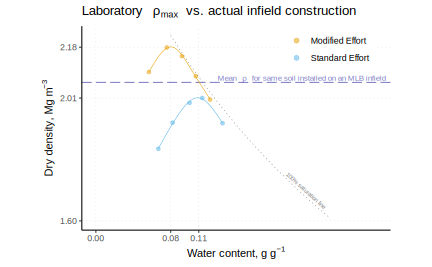
\includegraphics[width=0.9\linewidth]{../../cleatmarkmethod/figs/pdf/proctor-vs-observed-infield-density} 

}

\caption[Proctor tests compared with $\rho_{bulk}$ of an actual infield]{For a popular commercial infield mix, dry density values observed on a professionally managed infield surface lie between those achieved with the Standard and Modified Proctor tests.}\label{fig:proctor-vs-observed-infield-density}
\end{figure}

A pilot experiment was also performed to determine if a notable difference in sample behavior occurred between the two energy levels.
Two soils were used in this experiment.
These were mixed from the same sand and clay components to yield mixtures of 60 and 75\% sand.
Fresh batches of each air-dry soil were brought to their respective \(w_{opt}\) for the two energy levels.
The material was thoroughly hand-mixed with the appropriate mass of water and allowed to cure for ≥16 hr.

The soil was next compacted into the cleat-mark cylinders with the appropriate number of blows.
Due to the geometry of the cleat-mark cylinders this required a conversion for the compaction energy per unit volume of soil.
This calculation is detailed in the Appendix, Section \ref{cleat-mark-energy-per-vol-conversion}.
The standard routine used 2 lifts with 56 blows per lift.
The modified routine used 3 lifts with 63 blows per lift (See Equation \eqref{eq:modified-energy-per-volume-appendix}).

\hypertarget{comparison-of-density-achieved-during-proctor-tests-and-cleat-mark-compaction-routine}{%
\paragraph{Comparison of density achieved during Proctor tests and cleat-mark compaction routine}\label{comparison-of-density-achieved-during-proctor-tests-and-cleat-mark-compaction-routine}}

To validate the energy conversion, the masses and water contents of each prepared cleat-mark cylinder were recorded following compaction.
Three replicates of both soils at both energies were prepared, for a total of 12 specimens.

These were compared with the corresponding values of \(\rho_{max}\) derived from the original Proctor tests.

Figure \ref{fig:proctor-vs-cleat-mark-achieved-density-fig} shows that the three replicates within a soil-by-effort pair were very consistent. The pooled standard deviation for a soil-by-effort combination was just 0.007 Mg m\textsuperscript{-3}.
Figure \ref{fig:proctor-vs-cleat-mark-achieved-density-fig} also shows that the cleat-mark compaction routine packed the soil to a similar but systematically lower dry density than the corresponding Proctor tests.
This result agrees with other research on varying the mold diameter during compaction tests.
\protect\hyperlink{ref-ASTMD698-12}{ASTM International} (\protect\hyperlink{ref-ASTMD698-12}{2012}) states:

\begin{quote}
``Results have been found to vary slightly when a material is tested at the same compactive effort in different size molds, with the smaller mold size typically yielding larger values of density/unit weight.''
\end{quote}

\protect\hyperlink{ref-Johnson1962}{Johnson and Sallberg} (\protect\hyperlink{ref-Johnson1962}{1962}) compacted a clayey sand in variously-sized molds.
They reported a difference of 0.05 Mg m\textsuperscript{-3} between the 4" and 6" diameter molds.
This is very similar to the mean difference of 0.06 observed in this small experiment.
The small decrease in dry density should be expected given the specimen size.
Therefore, the energy conversion between the Proctor compaction mold and the cleat-mark cylinders was deemed valid.

\begin{figure}

{\centering \includegraphics[width=0.9\linewidth]{../../cleatmarkmethod/figs/pdf/proctor-vs-qc-density-comparison} 

}

\caption[$\rho_{max}$ for cleat-mark cylinders c.f. Proctor testing]{$\rho_{bulk}$ achieved with the cleat-mark cylinders was consistent across replications and slightly lower than $\rho$ derived from the corresponding Proctor curve.}\label{fig:proctor-vs-cleat-mark-achieved-density-fig}
\end{figure}

\hypertarget{trial-run-to-compare-compaction-routines}{%
\paragraph{Trial run to compare compaction routines}\label{trial-run-to-compare-compaction-routines}}

The next step in developing the specimen preparation routine was to determine whether the Standard or Modified routines would ultimately yield differences in the \(\theta_{crit}\) value corresponding with the cleat-in/cleat-out behavioral threshold.

Full trial runs of the cleat mark test were completed using each compaction routine.
The full procedure will be detailed in Section \ref{performing-cleat-mark-test}.
A single critical water content \(\theta_{crit}\) was derived for each soil-by-effort combination using the Normalized RFI as the surface metric of interest.
These values are presented in Table \ref{tab:derived-water-contents-from-cleat-mark-test-effort-comparison-tab}.
These data suggest the compaction effort does not markedly influence the ultimate value determined for \(\theta_{crit}\). The tests were not replicated so they cannot be statistically compared.

\begin{table}[htbp]

\caption[$\theta_{crit}$ values from cleat mark test performed with 2 compaction efforts]{\label{tab:derived-water-contents-from-cleat-mark-test-effort-comparison-tab}The critical volumetric water contents derived from the cleat mark test were nearly identical for the two compaction treatments.}
\centering
\begin{tabular}[t]{ccc}
\toprule
\multicolumn{1}{c}{\textbf{ }} & \multicolumn{2}{c}{\textbf{$\theta_{crit}$}} \\
\cmidrule(l{3pt}r{3pt}){2-3}
\textbf{Effort} & \textbf{60\% sand} & \textbf{75\% sand}\\
\midrule
Standard effort & 0.299 & 0.241\\
Modified effort & 0.299 & 0.233\\
\bottomrule
\end{tabular}
\end{table}

\hypertarget{summary---specimen-compaction}{%
\paragraph{Summary - specimen compaction}\label{summary---specimen-compaction}}

The Modified effort was ultimately adopted for all further study.
This choice is justified by the following:

\begin{enumerate}
\def\labelenumi{\arabic{enumi}.}
\item
  The ``critical'' water contents derived from the two methods were very similar (Table \ref{tab:derived-water-contents-from-cleat-mark-test-effort-comparison-tab}). No statistical comparison was made but the differences due to soil type appears to be larger than any difference due to compaction effort.
\item
  Soil bulk density on an actual infield was higher than that obtained from a Standard Proctor test, but lower than that obtained from a Modified Proctor test (Figure \ref{fig:proctor-vs-observed-infield-density}).
  The prevailing view among baseball grounds managers is that the infield should be as compacted as possible.
  Therefore, a realistic lab test should favor greater rather than lesser compaction.
\end{enumerate}

\hypertarget{performing-cleat-mark-test}{%
\subsubsection{Performing the test}\label{performing-cleat-mark-test}}

There are four basic steps in the cleat-mark test:

\begin{enumerate}
\def\labelenumi{\arabic{enumi}.}
\item
  Produce cleat indentations on the specimen
\item
  Collect a 3D scan
\item
  Measure the water content and some additional features of the sample.
\item
  Repair the specimen for subsequent tests
\end{enumerate}

\hypertarget{cleat-indentations}{%
\paragraph{Cleat indentations}\label{cleat-indentations}}

The pneumatic device is first charged to 690 kPa (100 psi).
The specimen is secured into the device with adjustable clips.
The device is manually actuated and then retracted.
Any soil ejected from the cleat indentations is carefully removed so that the clods are not crushed by subsequent tests.
This sequence is repeated twice more, rotating the specimen by 60 ° after each test.
The reserved soil clods are carefully replaced at their original locations.

\hypertarget{cleat-mark-specimen-3D-scanning}{%
\paragraph{3D scan}\label{cleat-mark-specimen-3D-scanning}}

Six markers are placed on the rim of the aluminum sample holder.
The markers allow the scanner to register each pointcloud and merge them into a single mesh.
A series of scans is made using a step size of 20° for a total of 18 captures per specimen.
These are merged using EinScan's software (without scaling or reduction) and exported as a single \texttt{.ply} file.
The \texttt{.ply} format is an open file format and supports both ASCII and binary encoding (\protect\hyperlink{ref-Turk1994}{Turk, 1994}).

\hypertarget{water-content-and-ancillary-data}{%
\paragraph{Water content and ancillary data}\label{water-content-and-ancillary-data}}

Representative values of \(w\) and \(\theta\) are determined using the procedure detailed in Section \ref{sand-replacement-vs-scanner-for-theta}.

Penetrometer resistance is measured with a handheld device having a maximum capacity of 5 kg cm\textsuperscript{-1}.
Four readings are averaged to produce a a representative value.
Dry specimens tend to reject this device, so in these cases peak resistance cannot be recorded.
Visual observations on the nature of deformation are noted.
Finally, a digital photograph of the sample is taken after the test.

\hypertarget{specimen-repair}{%
\paragraph{Specimen repair}\label{specimen-repair}}

Several data points are needed to define \(\theta_{crit}\).
The samples are wetted and allowed to cure overnight.
The cleat indentations are then repaired with soil pre-wetted to \(w_{opt}\).
This procedure effectively refreshes the surface to its initial state.
The repairs are made with a routine similar to that used on real infields.
Figure \ref{fig:daily-specimen-repair-panels} shows this process.



\begin{figure}

{\centering \includegraphics[width=0.9\linewidth]{figs/png/daily-specimen-repairs-panels} 

}

\caption[Repair proces for cleat-mark specimens]{\textbf{A.} The soil is scarified to a depth of 20 mm to facilitate binding with the new material. \textbf{B.} Additional material is added and compacted with a Proctor hammer. \textbf{C.} The soil is planed to the specimen rim with a straight edge. \textbf{D.} The specimen is thoroughly wetted before repeating the drydown procedure described in Section \ref{measuring-and-adjusting-water-content}.}\label{fig:daily-specimen-repair-panels}
\end{figure}

\hypertarget{measuring-and-adjusting-water-content}{%
\subsubsection{Measuring \& adjusting the water content}\label{measuring-and-adjusting-water-content}}

Wetting and drying cycles are an important part of infield behavior.
The brittle-ductile transition mostly occurs during day games when no water can be added after the game begins.

A given soil must be tested at a range of water contents which bracket \(\theta_{crit}\).
In our lab test, the water content was adjusted up or down by adding a known volume of water or by drying under a heat lamp manifold.
The manifold was calibrated to emulate the outdoor conditions on a summer day in the northeastern United States.
Figure \ref{fig:heat-lamps-photo} shows the apparatus which comprises 12 clamp fixtures on 60 cm spacing. Each fixture houses a 150-W broad-spectrum incandescent bulb (Exo-Terra PT2114 - A21/150W).

Proper configuration of the drying apparatus was determined through a series of calibrations.
These measured the effect of lamp distance, the variability in water content within and across specimens, and the validity of two methods for measuring \(\theta\).
These are next described.

\hypertarget{water-content-study-1-lamp-distance}{%
\subparagraph{Water content study 1: Lamp distance}\label{water-content-study-1-lamp-distance}}

The goal of this experiment was to determine the proper distance between the heat source and the soil surface.
Gravimetric water content \(w\) was determined in the top 15 mm using an 8 mm diameter soil probe.
Four samples were extracted each hour and averaged to produce a representative value for the surface.
The surface temperature was also recorded using an infrared laser thermometer.
The first 3-4 hours of drying are of greatest interest be cause this is the typical length of a professional baseball game.

Figure \ref{fig:water-content-change-by-lamp-height} A shows that the distance between the heat bulb and the soil specimen markedly affects the drying rate.
A 15 cm distance caused excessively rapid drying (initially over 3 \% by dry mass hr\textsuperscript{-1}).
Figure \ref{fig:water-content-change-by-lamp-height} B also shows the rate of water loss was not constant with time.
Water loss was most rapid during the first ≈ 2.5 hours before tapering off.
This is a well-documented phenomenon in soil physics and often corresponds with the breaking of continuous capillary flow (\protect\hyperlink{ref-Radcliffe2010}{Radcliffe and Simunek, 2010}).

At the other extreme, the 45 cm lamp height produced only a small change in water content over several hours.

The 30 cm distance produced the most realistic result.
\(\Delta_w\) was 0.032 over the first 2.75 hr.
Figure \ref{fig:lamp-height-calibration} shows that the surface temperature observed beneath the 30 cm lamp height compared favorably with that of an actual infield on a sunny August day in Pennsylvania.

\begin{figure}

{\centering \includegraphics[width=0.9\linewidth]{./images/heat-lamps} 

}

\caption{Drydown manifold used prior to cleat-mark test.}\label{fig:heat-lamps-photo}
\end{figure}

\begin{figure}

{\centering \includegraphics[width=0.9\linewidth]{../../cleatmarkmethod/figs/manually-built/drydown-surface-temp-comparison} 

}

\caption[Temperature beneath drydown apparatus c.f. outdoor conditions]{Surface temperature for the 30 cm lamp height closely matches conditions observed on a sunny day in Pennsylvania (outdoor photo credit: Andrew Burnette)}\label{fig:lamp-height-calibration}
\end{figure}

\begin{figure}

{\centering \includegraphics[width=0.9\linewidth]{04-Proposed-experiments_files/figure-latex/water-content-change-by-lamp-height-1} 

}

\caption[Changes in total $w$ and evaporation rate with time]{\textbf{A.} Water loss was most significant for the 15 cm height. \textbf{B.} The first derivative of $w$ with respect to time shows the rate of water loss changed rapidly for the lowest lamp height. The 30 and 45 cm heights lost water at a steadier rate.}\label{fig:water-content-change-by-lamp-height}
\end{figure}

\hypertarget{water-content-study-2-uniformity-across-specimen-surface-and-across-replicate-specimens}{%
\subparagraph{Water content study 2: Uniformity across specimen surface and across replicate specimens}\label{water-content-study-2-uniformity-across-specimen-surface-and-across-replicate-specimens}}

The cleat-mark test pairs a single water content value with a surface disruption measurement.
In water content study (1), \(w\) was assumed to be equal across the specimen surface.
A second experiment was performed to verify this assumption.

As for water content study (1), \(w\) was determined in the top 15 mm using an 8 mm diameter soil probe.
A 40-mm grid was marked on three replicate specimens. The samples were placed under the drying apparatus and a soil sample was removed at each grid intersection every 60 minutes (Figure \ref{fig:water-content-grid-photo}).
This allowed comparison of \(w\) across both space and time.

Figure \ref{fig:w-variation-across-space-and-time} shows the results for each replicate during the 6-hr drying period.
The water content was highly uniform across the surface of a single specimen, and the difference across replications was small.
Therefore, it is reasonable to consider the water content horizontally uniform for a single specimen.

\begin{figure}

{\centering \includegraphics[width=0.9\linewidth]{images/w-grid-sampling} 

}

\caption{Grid sampling for water content study (2).}\label{fig:water-content-grid-photo}
\end{figure}

\begin{figure}

{\centering \includegraphics[width=0.9\linewidth]{figs/pdf/w-variation-across-space-and-time} 

}

\caption[Spatial and temporal variation of $w$ for cleat-mark cylinders]{$w$ was consistent across the surface of a single specimen and across replicate cylinders.}\label{fig:w-variation-across-space-and-time}
\end{figure}

\hypertarget{sand-replacement-vs-scanner-for-theta}{%
\subparagraph{\texorpdfstring{Water content study 3: Precise measurement of \(\theta\)}{Water content study 3: Precise measurement of \textbackslash theta}}\label{sand-replacement-vs-scanner-for-theta}}

The third water content study's aim was to develop a method for measuring \emph{volumetric} water content \(\theta\).
Relative merits of \(w\) and \(\theta\) are discussed in Section \ref{soil-water-content} and by \protect\hyperlink{ref-Brady2007}{Brady and Weil} (\protect\hyperlink{ref-Brady2007}{2007}).
In the present study it is far easier to measure \(w\) on the small samples available for testing.
However, it is the volume of water which determines the spacing of soil particles and the nature of their contacts.
Also, \(\theta\) is more commonly in use among grounds managers because it can be measured in-situ on an actual infield with a time-domain reflectometry probe.
It would be preferrable to use \(\theta\) over \(w\) if it can be precisely measured.
Therefore a method was sought to measure \(\theta\) using small samples.
The goal was to compute \(\theta\) as \(w \cdot \rho_{bulk}\).

A small intact soil core was removed (diameter = 21mm, depth = 15 mm) using a soil probe (Figure \ref{fig:mini-density-panels}).
The core is ejected with a plunger and immediately weighed to ± 0.001 g.
The bottom of the core normally separates in an uneven pattern, so a simple geometric computation
of the cylinder's volume is not possible.
Two methods were employed to measure the volume of the plug:

(1.) Sand replacement

(2.) 3D scanning

\begin{figure}

{\centering \includegraphics[width=0.95\linewidth]{figs/png/mini-density-combined-panels} 

}

\caption[Measuring the volume of miniature soil plugs]{Measuring the volume of a 15 mm-deep by 21 mm diameter soil plug: \textbf{A.} Miniature soil probe and plunger. \textbf{B.} Sand replacement method with an inverted cone. \textbf{C}. 3D scanning method with plug situated on a rest to provide clearance from turn table.}\label{fig:mini-density-panels}
\end{figure}

Method (1) was essentially a miniature version of ASTM D1556 (\protect\hyperlink{ref-ASTMD1556-07}{2014b}).
A small plastic cone was trimmed and its volume was carefully calibrated with de-aired water.
A dry sand was calibrated to loose density of 1.54 Mg m\textsuperscript{-3}.
These were used to fill the cavity left by the soil plug (Figure \ref{fig:mini-density-panels} B).
The plug volume was calculated from the mass of sand used to fill the hole and the known cone volume:

\begin{align}
\quad V_{plug} &= V_{sand_{~total}} - V_{cone} \quad ; \quad V_{sand_{~total}} = \frac{m_{sand_{~total}}}{\rho_{sand}} \\
V_{plug} &= \frac{m_{sand_{~total}}}{\rho_{sand}} - V_{cone}
\label{eq:mini-density-sand-backfill-equation}
\end{align}

In method (2), a 3D scan of the core was recorded (Figure \ref{fig:mini-density-panels} C).
3D scanning has been used to measure bulk density for irregularly-shaped soil clods (\protect\hyperlink{ref-Rossi2008}{Rossi et al., 2008}). The scanning process was similar to that described for the actual cleat-mark test (Section \ref{cleat-mark-specimen-3D-scanning}).
The primary difference was that for the water content plug scan, two scans were recorded with the plug in different orientations.
This was required for all sides to be ``seen'' by the scanner.
An additional challenge was raising the specimen above the turntable so it would register separately from the turntable.
Ultimately the plug was stationed atop a \#10 U.S. hex nut. This resting space provided enough clearance so the soil could be differentiated from the turntable while maintaining a stable orientation.
The volume of the plug was determined using the \texttt{vcgVolume()} function in the \textbf{\texttt{Rvcg}} software package for R (\protect\hyperlink{ref-Schlager2017}{Schlager, 2017}).

For both plug volume methods, a \(\theta\) value was computed from the specimen's gravimetric water content and its dry density:

\begin{align}
% \text{Gravimetric water content:}  \nonumber  \\ 
w &= \frac{water~loss~(g)}{m_{oven-dry~soil}~(g)} \\
% \text{Dry bulk density:}  \nonumber  \\
\rho_{bulk} &= \frac{m_{oven-dry~soil}~(g)}{core~volume~(cm^3)} \\
% \text{Volumetric water content:} \nonumber \\
\theta  = \rho_{bulk} \times w &= \frac{water~loss~(g)}{m_{oven-dry~soil}~(g)} \times \frac{m_{oven-dry~soil}~(g)}{core~volume~(cm^3)}
\label{eq:vwc-equation} 
\end{align}

5 replicate soil plugs were analyzed on each of the 12 prepared cleat-mark specimens.
Mean values and standard deviations were computed for each method; these data are plotted in Figure \ref{fig:sand-backfill-vs-3D-scanner-for-volumetric-w-determination-fig} and the values are compiled in the Appendix (Table \ref{tab:sand-backfill-vs-3D-scanner-for-volumetric-w-determination-table}).



\begin{figure}

{\centering \includegraphics[width=0.9\linewidth]{../../cleatmarkmethod/figs/pdf/mini-plug-density-comp} 

}

\caption[$\rho$ obtained from 3D scanning and sand replacement]{The 3D scanning method for computing the extracted plug's volume was more repeatable than the sand-backfill method. the 3D scanning method also yielded higher mean \(\rho_{bulk}\) for 11 of the 12 cylinders.}\label{fig:sand-backfill-vs-3D-scanner-for-volumetric-w-determination-fig}
\end{figure}

Figure \ref{fig:sand-backfill-vs-3D-scanner-for-volumetric-w-determination-fig} shows improved precision with the scanner method.
The standard deviation \(\sigma_{\rho}\) for a single specimen was 0.07 when measured with sand replacement, but only 0.03 when measured with the scanner.
Therefore, computing \(\rho\) with the 3D scanning method reduces error propagation in \(\theta\).
As an example, if the true value for \(w\) is 15\%, the consequence of one standard deviation of 0.07 Mg m\textsuperscript{-3} in the density measurement propagates to a \(\theta\) error of 0.011. This would appear unacceptably large if the cleat-mark analysis is to pinpoint \(\theta_{crit}\) within \textless{} 1 \% accuracy.

Interestingly, the scanner method produced not only less scatter but also higher mean \(\rho_{bulk}\) for 11 of the 12 cylinders.
The average difference was 0.053 Mg m\textsuperscript{-3}. Most likely the probe produces some plastic distortion of the hole's sidewalls when it is inserted and removed.
This additional space is filled by sand which increases the measured volume and decreases the computed dry density.
Also, for this small sample diameter the probe's sidewalls (0.5 mm) comprise a non-negligible fraction of the total hole's volume.
Again, this volume is considered part of the plug volume for the sand replacement method but not for the scanner method.

The scanner method directly measures the volume of the soil plug, so it more accurately represents the soil sample's true dimensions.
Intact core sampling is often assumed to produce some compaction in the sidewalls as the probe is driven into the surface (\protect\hyperlink{ref-Lichter1994}{Lichter and Costello, 1994}).
These samples are already intentionally compacted to a high degree so the sidewall compaction effect is probably minor.

\hypertarget{summary-measuring-and-adjusting-water-content}{%
\subparagraph{Summary: measuring and adjusting water content}\label{summary-measuring-and-adjusting-water-content}}

A routine was developed to wet and dry the samples in a controlled manner.
A set of heat lamps dries the surfaces uniformly across space.
\(\theta\) can be measured with good precision and accuracy by using a combination of gravimetric methods and 3D scanning.

\hypertarget{mesh-processing-pipeline}{%
\subsubsection{Mesh processing pipeline}\label{mesh-processing-pipeline}}

In their raw state, the \texttt{.ply} files are of little use because their coordinates are relative to the scanner's detector, not a ``real-world'' coordinate system.
They also contain incomplete fragments of the aluminum specimen holder.
Figure \ref{fig:orienting-and-removing-cyl-fig} A shows the raw mesh in ``real-world'' coordinates immediately following the scan acquisition.
A number of cleaning and processing operations are required before collecting any surface measurements.

Mesh processing may be done interactively with point-and-click software such as MeshLab (\protect\hyperlink{ref-Cignoni2008}{Cignoni et al., 2008}), but this interactive approach does not scale to large numbers of meshes and it is subject to human error.
Instead, a processing routine was developed using the R Language for Statistical Computing (\protect\hyperlink{ref-R-core2021}{R-Core-Team, 2021}).
The routine is stored in the author's \textbf{\texttt{soilmesh}} package (\url{https://github.com/evanmascitti/soilmesh}).
\textbf{\texttt{soilmesh}} is primarily based on the \textbf{\texttt{Rvcg}} and \textbf{\texttt{Morpho}} packages (\protect\hyperlink{ref-Schlager2017}{Schlager, 2017}), which are in turn built atop the open-source C++ libraries maintained by the ISTI-CNR Visual Computing Lab (Pisa, Italy, \url{https://www.isti.cnr.it/en/}).
A 4x4 roto-translation matrix was interactively recorded using a freshly prepared specimen.
This 4x4 matrix was saved as an \texttt{.rda} data file and applied to each mesh using implicit loops (functionals).
Figure \ref{fig:orienting-and-removing-cyl-fig} B) shows the corrected orientation of the mesh.

The mesh was then finely adjusted in the x-y plane based on its maximum x and y coordinate values.
This step is required because it is impossible to place each successive specimen in an \emph{identical} location on the turntable.
Next, any points greater than 70 mm from the mesh's center were removed by computing Boolean values for each vertex solved from the basic equation for a circle with origin \((0,0)\) :

\begin{align}
        \begin{split}
            (x - h)^2 + (y - k)^2 &= r^2 \\
            \mathrm{Since}~x=0~\mathrm{and}~y=0;~~ (x - 0)^2 + (y - 0)^2 &= 70^2 \\
            x^2 +y^2 &= 70^2 \\
        \end{split} 
\label{eq:cylinder-clipping-equation} 
\end{align}

Therefore for a given vertex, if \(x^2+y^2>70^2\) the vertex was removed from the matrix of coordinates.
This step ``trimmed'' both the aluminum sample holder and the outer rim of the specimen's surface, leaving a disk 140 mm in diameter (Figure \ref{fig:orienting-and-removing-cyl-fig} C).

After removing the cylinder a final adjustment was made to the mesh's z-coordinates.
Fine-grained soil may change volume as it wets or dries.
The change is not necessarily planar; the center of the sample often shrinks faster than the edges.
These small changes in surface elevation mean that a single rigid 4x4 matrix cannot return the ``origin'' of every sample to the exact coordinates \((0, 0, 0)\).
However, it could be assumed that \emph{on average} the elevation with the greatest frequency of points represents the elevation of the original soil surface at test time.
This assumption was used to perform the final z-adjustment.
The distribution of z-coordinates (comprising \textasciitilde2.5 million points) was split into 10,000 bins.
The most frequently occurring value was assumed to be the ``true'' level of z=0.
Each point in the mesh was moved up or down by this value, depending on its sign (Figure \ref{fig:mesh-z-points-histogram}).

\begin{figure}

{\centering \includegraphics[width=0.9\linewidth]{../../cleatmarkmethod/figs/pdf/z-histogram} 

}

\caption[Final adjustment of mesh z-coordinates]{Each vertex of the mesh was adjusted by the median elevation to further refine the position of the mesh.}\label{fig:mesh-z-points-histogram}
\end{figure}

The result of the orientation, cleaning, and decimation operations is shown in Figure \ref{fig:orienting-and-removing-cyl-fig} C.
The ``origin'' of the mesh lies within a fraction of 1 mm from \((0, 0, 0)\).



\begin{figure}

{\centering \includegraphics[width=0.9\linewidth]{../../cleatmarkmethod/figs/manually-built/processing-pipeline-panel} 

}

\caption[Mesh orientation and cleaning pipeline]{\textbf{A.} Orientation of the raw mesh generated by 3D scanner. \textbf{B.} Orientation of the specimen after application of 4x4 roto-translation matrix. \textbf{C.} Final orientation of mesh after removing extraneous portions and performing secondary position adjustments. Junction of the three axes represents \((0,0,0)\).}\label{fig:orienting-and-removing-cyl-fig}
\end{figure}

\hypertarget{mesh-size-reduction}{%
\paragraph{Mesh size reduction}\label{mesh-size-reduction}}

The final step in the pre-processing routine is to reduce the size of the \texttt{.ply} file.
Landscape-scale research has shown that large pointclouds often have resolution exceeding that required for robust analyses (\protect\hyperlink{ref-Brubaker2013}{Brubaker et al., 2013}).
In such a case, it is pragmatic to reduce the file sizes for easier storage and better computational efficiency.

A decimating ``titration'' was performed on several meshes to determine how much the mesh size could be reduced without sacrificing detail.
Figure \ref{fig:decimation-titration-surface-area} shows that for a raw mesh file with \textgreater{} 3 million faces, little loss in surface area occurred until the mesh was reduced to ≈100,000 faces.
A face number of 500,000 was chosen to include a factor of safety.

\begin{figure}

{\centering \includegraphics[width=0.9\linewidth]{../../cleatmarkmethod/figs/pdf/surface-area-by-faces-titration} 

}

\caption[Mesh decimation to reduce file size.]{Meshes were decimated to 500,000 faces (red vertical line) to impove computational efficiency without a loss in data quality.}\label{fig:decimation-titration-surface-area}
\end{figure}

\hypertarget{summary-mesh-processing-pipeline}{%
\paragraph{Summary: mesh processing pipeline}\label{summary-mesh-processing-pipeline}}

The processing routine is a substantial advance compared with point-and-click alternatives.
By performing the mesh processing programatically, time is saved and the results are made operator-independent.

\hypertarget{surface-metrics}{%
\subsubsection{Surface metrics}\label{surface-metrics}}

A primary goal of baseball grounds managers is to minimize disturbance to the infield skin during play.
In the cleat-mark test, several measurements have been developed to enumerate the degree of disturbance to the soil surface.
All are conceptually referenced to an undisturbed soil surface of the same radius, lying in the \((x, y)\) plane (Figure \ref{fig:ref-circ-plane-fig}).

\begin{figure}

{\centering \includegraphics[width=0.5\linewidth]{figs/png/ref-circ-plane} 

}

\caption[3D mesh of undisturbed soil surface]{3D mesh of undisturbed soil surface centered at $(0,0,0)$}\label{fig:ref-circ-plane-fig}
\end{figure}

Figure \ref{fig:example-meshes-panels} shows the range of surface conditions produced during the test.
These three meshes were produced from the same soil at different water contents.

\begin{figure}

{\centering \includegraphics[width=0.9\linewidth]{../../cleatmarkmethod/figs/png/example-high-medium-low-surface-area-meshes} 

}

\caption[Example 3D meshes after testing.]{(Top to bottom): Examples of surfaces with high, moderate, and low surface disruption. Meshes in a row are equivalent. Colors at right are mapped to the points' z-coordinates, with red areas lying above the reference plane and blue areas below.}\label{fig:example-meshes-panels}
\end{figure}

The measurements are grouped into three categories:

\textbf{Surface metric group 1.} Volume of disturbed soil

Effectively these are the ``cut'' or ``fill'' required to return the tested sample to its originally planar state. Several algorithms were developed to compute these values from the pointcloud (voxel-based sampling, rasterization, and full re-meshing).

\begin{figure}

{\centering \includegraphics[width=0.9\linewidth]{../../cleatmarkmethod/figs/png/top-view-plan-view-combined.png  } 

}

\caption[3D mesh split by vertex elevations]{Soil volume was computed for portions of the mesh lying either above or below the reference datum.}\label{fig:volume-slicing-fig}
\end{figure}

Mesh-generated volumes were compared with a physical analog method.
Volume above the datum was computed by collecting any disturbed clods from the soil surface.
If no clods were ejected, material which was plastically deformed above the cylinder rim was shaved off with a metal rule.
The supra-datum soil was oven-dried and weighed, and supra-datum volume was computed from its oven-dry mass and \(\rho\).

The sub-datum volume was computed using a sand-backfill method similar to ASTM D-1556 (\protect\hyperlink{ref-ASTMD1556-07}{2014b}).
The depressions were back-filled with dry sand of known \(\rho\) and the volume was computed from the mass of sand used to fill the depressions (Figure \ref{fig:cleat-mark-sand-backfill-panel}).

\begin{figure}

{\centering \includegraphics[width=0.9\linewidth]{figs/png/cleat-mark-sand-backfill-panel} 

}

\caption[Sand backfill method for cleat-mark volume]{Manual sand-backfilling method for computing sub-datum volume.}\label{fig:cleat-mark-sand-backfill-panel}
\end{figure}

\textbf{Surface metric 2.} Normalized Relief Index (NRFI)

This is the simplest of the measurements - it is a normalized ratio of the triangular mesh's 3D surface area to its 2D footprint.
The surface area of the reference plane is subtracted and the result is multiplied by 100 to make the values simpler to compare.
NRFI is essentially the percent gain in surface area for the tested specimen over its undisturbed equivalent. The formula is:

\begin{equation}
NRFI = \left(\frac{\text{surface area}_{\text{ total}}}{\pi~r^2} - \pi~r^2 \right) \times 100 \\
\label{eq:nrfi-equation} 
\end{equation}

\textbf{Surface metric 3.} Dirichlet Normal Energy (DNE)

Dirichlet Normal Energy is a more complex morphometric used in anthropology and biology.
In particular, it has been used to quantify surface roughness of primate dentition (\protect\hyperlink{ref-Bunn2011}{Bunn et al., 2011}).
DNE is a measure of the total curvature of a surface: a horizontal plane has DNE of zero.
For each point on a surface, DNE computes two principal curvatures and compares them with a plane oriented perpendicular to the vertex normal.
For regular geometries (such as a sphere) the total DNE is integrable, but for irregular surfaces a discretization is required.
The \texttt{molaR} package for R (\protect\hyperlink{ref-Pampush2020}{Pampush et al., 2020}) computes DNE from \texttt{.ply} meshes.
The discretization is performed by using the face normals rather than vertices.
The DNE value for each face is multiplied by its surface area and these values are summed to produce a whole-surface value.
See \protect\hyperlink{ref-Pampush2016}{Pampush et al.} (\protect\hyperlink{ref-Pampush2016}{2016}) and \protect\hyperlink{ref-Bunn2011}{Bunn et al.} (\protect\hyperlink{ref-Bunn2011}{2011}) for a more detailed treatment of DNE.

\hypertarget{determination-of-theta_crit}{%
\subsubsection{\texorpdfstring{Determination of \(\theta_{crit}\)}{Determination of \textbackslash theta\_\{crit\}}}\label{determination-of-theta_crit}}

The goal of the cleat-mark test is to identify a single water content where the soil exhibits an abrupt change between brittle and ductile behavior.

Each surface metric was plotted against volumetric water content.
For this discussion NRFI is referenced as the metric of choice, but the general shape of the relationship is similar for other metrics.
Figure \ref{fig:example-nrfi-vs-water-content-curve} shows an example curve.
A third-order polynomial regression was fitted to a plot of NFRI against \(\theta\).
The critical water content \(\theta_{crit}\) was identified as the first local minimum as the soil moves from wet to dry (right to left on Figure \ref{fig:example-nrfi-vs-water-content-curve}).



The choice of this point as \(\theta_{crit}\) warrants a brief discussion behind the physical meaning of the curve's shape.

\begin{figure}

{\centering \includegraphics[width=0.9\linewidth]{./figs/pdf/example-w-crit-curve} 

}

\caption[Conceptual stages of infield soil behavior with reducing $\theta$]{An example of the characteristic water contents used to derive \(\theta_{crit}\). Water contents above point A generally yield little additional disturbance. Water content B represents the state in which the soil is most `vulnerable' to fragmentation. As water content reduces further toward point C, the soil hardens and the cleats are less able to penetrate the surface.}\label{fig:example-nrfi-vs-water-content-curve}
\end{figure}

When the soil is very wet, the device easily actuates to the full extent afforded by its geometry.
Further increases in the water content can only produce a marginally greater disruption to the specimen. The NRFI vs.~\(\theta\) curve is relatively flat.

At lower water contents, disturbance is relatively constant because no soil is removed or fractured from the surface.
Any new surface area is governed purely by the shape of the cleats.
This is an ideal state from the perspective of the grounds manager.

When the soil reaches \(\theta_{crit}\) it begins to fragment into discrete pieces as the cleats penetrate the surface.

As the soil continues to dry, brittleness is maximized and the soil forms larger chips and clods.
These may fragment further which produces additional surface area.

A possible complication not depicted in Figure \ref{fig:example-nrfi-vs-water-content-curve} is that with further decreases in water content the soil becomes so hard that NFRI falls below its value at \(\theta_{crit}\).
Although NFRI is nominally lower in this state, the soil is in an undesirable condition because of its high strength.
Ball response will be erratic and players can incur injuries due to extreme surface hardness.
For this reason, any points drier than the local maximum marked as point (B) in Figure \ref{fig:example-nrfi-vs-water-content-curve} are discarded prior to optimizing the curve to derive \(\theta_{crit}\).

\hypertarget{summary-cleat-mark-method}{%
\subsubsection{Summary: cleat-mark method}\label{summary-cleat-mark-method}}

\begin{itemize}
\item
  The method described above provides an objective means to choose a single water content for any infield soil. This value is termed \(\theta_{crit}\).
\item
  \(\theta_{crit}\) is considered the lower boundary of the water contents suitable for play.
\item
  A standard routine was adopted for building and repairing the soil specimens. The routine uses techniques similar to those empolyed on actual infields, including the Modified Proctor hammer and a drying apparatus to emulate natural sunlight.
\item
  It is recognized that the shape of the disturbance metric vs.~water content curve may not be equivalent for all soils. The curve-fitting routine merits further study.
\end{itemize}

\hypertarget{timeline}{%
\subsection{Timeline}\label{timeline}}

The device was designed and fabricated in spring 2020. Calibration and tuning of the 3D scanner began July of 2020. The method described above has been tested on multiple soils. The final step will be to perform an error analysis across replicate soil specimens.

\newpage

\hypertarget{paper-2-applying-the-cleat-in-cleat-out-method}{%
\section{Paper 2: Applying the cleat-in, cleat-out method}\label{paper-2-applying-the-cleat-in-cleat-out-method}}

\begin{description}
\item[Paper title:]
\textbf{Identifying the brittle-ductile transition of infield soil mixtures subjected to disturbance by baseball cleats}
\end{description}

\hypertarget{overview-1}{%
\subsection{Overview}\label{overview-1}}

This paper is the first chance to apply the method described in Section \ref{cleatmark-method-development-chapter}.

\hypertarget{principal-research-questions-1}{%
\subsection{Principal research questions}\label{principal-research-questions-1}}

\begin{enumerate}
\def\labelenumi{\arabic{enumi}.}
\item
  How does clay type interact with sand content to determine the critical water content corresponding to the cleat-in/cleat-out behavioral threshold?
\item
  For a given clay soil, what is the critical sand content above which the cleat-in/cleat-out surface cannot be achieved?
\end{enumerate}

\hypertarget{hypotheses-1}{%
\subsection{Hypotheses}\label{hypotheses-1}}

\hypertarget{materials-and-methods-1}{%
\subsection{Materials and Methods}\label{materials-and-methods-1}}

This paper consists of three separate experiments. They are designed to test the effect of:

\begin{enumerate}
\def\labelenumi{\arabic{enumi}.}
\tightlist
\item
  \textbf{Varying sand content:} Five fine-grained soils will be mixed with a single sand in ratios ranging from 50-80\% sand.
  Sand contents will be clustered around the transitional fines content to help identify the critical behavioral threshold for each clay type (see Figure \ref{fig:sand-content-clustering}).
  This is preferred to simply testing mixes with equally-spaced sand contents, because the behavior change is nearly linear up to the transitional fines content (see Section \ref{coarse-fraction-effects-on-soil-mixtures}).
  This range of sand content is slightly larger than standard recommendations for infield mixes.
  Therefore, standard materials can be compared with border cases.
\end{enumerate}

\begin{figure}

{\centering \includegraphics[width=0.9\linewidth]{figs/pdf/sand-pcts-to-choose} 

}

\caption[Clustering of sand contents for best data resolution]{The sand contents for Experiment 1 in Chapter 2 will be deliberately clustered around the transitional fines content to provide the best data resolution}\label{fig:sand-content-clustering}
\end{figure}

\begin{enumerate}
\def\labelenumi{\arabic{enumi}.}
\setcounter{enumi}{1}
\tightlist
\item
  \textbf{Varying silt-to-clay ratio:} The same fine-grained soils from (1) will each be separately mixed with quartz silt to produce soil mixtures having identical silt-to-clay ratios (SCR) but containing different clay minerals.
  These soils will be further mixed with sand to produce mixtures of either 60 or 70\% sand.
  The target SCR values will be 0.25, 0.5, 1, 2, and 4, but some of the clays already contain too much silt to be tested at the lower SCR values.
  These soils would simply be tested at any ratios they are capable of meeting (Table \ref{tab:planned-scr-values}).
\end{enumerate}

\begin{table}

\caption[Adjusted silt-to-clay ratios of "pure" clays]{\label{tab:planned-scr-values}The 5 soils from Experiment 1 have different silt-to-clay ratios; silt can be added to produce soils with equivalent SCR values but different clay minerals and clay particle sizes. High-silt soils cannot be tested at an SCR lower than their existing value.}
\centering
\begin{tabular}[t]{lccc}
\toprule
\multicolumn{1}{c}{ } & \multicolumn{3}{c}{Approximate particle-size parameters} \\
\cmidrule(l{3pt}r{3pt}){2-4}
\textbf{Clay name} & \textbf{\% Clay-size} & \textbf{\% Silt-size} & \textbf{Silt-to-clay ratio}\\
\midrule
Fine-grained kaolinite & 0.80 & 0.20 & 0.25\\
Sesquioxide-rich & 0.80 & 0.20 & 0.25\\
Calcium montmorillonite & 0.60 & 0.40 & 0.67\\
Mixed-layer/illite-dominated & 0.50 & 0.50 & 1.00\\
High-silt soil & 0.10 & 0.90 & 9.00\\
\bottomrule
\end{tabular}
\end{table}

\begin{enumerate}
\def\labelenumi{\arabic{enumi}.}
\setcounter{enumi}{2}
\tightlist
\item
  \textbf{Varying sand type:} Two of the clays from Experiment (1) will be chosen based on having high and low toughness.
  They will be mixed with 4 types of sand at 4 sand contents (50, 60, 70, and 75\%) for a total of 32 mixes.
  The sand types include a ``coarse,'' ``medium'' and ``fine'' with similar uniformity coefficients \(C_u\) and a fourth sand having similar D\textsubscript{50} to the ``medium'' sand but a larger \(C_u\).
  This design allows a comparison of both size and uniformity to be made for a both low- and high-toughness clays.
\end{enumerate}

\hypertarget{timeline-1}{%
\subsection{Timeline}\label{timeline-1}}

These experiments will be conducted throughout Summer and Fall 2021 (see Figure \ref{fig:gantt-chart}).

\newpage

\hypertarget{paper-3-toughness-of-sand-clay-mixtures}{%
\section{Paper 3: Toughness of sand-clay mixtures}\label{paper-3-toughness-of-sand-clay-mixtures}}

\begin{description}
\item[Paper title:]
\textbf{Toughness-water content relations of clay soils via unconfined compression testing}
\end{description}

\hypertarget{overview-2}{%
\subsection{Overview}\label{overview-2}}

Infield soils have two critical water contents that define the range of acceptable consistency. The lower boundary is defined by the cleat-in/cleat-out behavioral threshold. Chapters 1 and 2 address the lower boundary.

The upper boundary of water content is governed by toughness and shear strength.
Although much emphasis has been given to the cleat-in/cleat-out threshold, this upper boundary of water content has more serious implications. Above this water content the game simply cannot be played.
Section \ref{importance-of-the-infield} described the financial and scheduling implications of postponements.

This paper is the compliment to Section \ref{cleatmark-method-development-chapter}.
Its goal is to create a new way to use existing tests for measuring the toughness of soil mixtures.
Together, these data can establish both ends of the water content spectrum for a given soil.

The method development for this paper will not be nearly as intensive as that of Paper 1.
For the most part, the techniques already exist and I am simply planning them in a new way.

\hypertarget{principal-research-questions-2}{%
\subsection{Principal research questions}\label{principal-research-questions-2}}

\begin{enumerate}
\def\labelenumi{\arabic{enumi}.}
\item
  Can soil toughness be measured using unconfined compression tests?
\item
  How does toughness vary with water content for different types of clay soils?
\item
  How does the toughness-water content relationship change as sand is added to the clays?
\end{enumerate}

\hypertarget{hypotheses-2}{%
\subsection{Hypotheses}\label{hypotheses-2}}

\begin{enumerate}
\def\labelenumi{\arabic{enumi}.}
\item
  Soil toughness can be measured with unconfined compression tests. By testing both specimens dry and wet of the plastic limit, one can interpolate their maximum toughness, which occurs at the plastic limit (i.e.~onset of brittle fracturing).
\item
  Higher plasticity soils will have less change in toughness for a unit change in water content. The maximum toughness of the clay types will be in order of montmorillonite \textgreater\textgreater{} mixed-layer/illite \textgreater{} kaolinite \textgreater{} iron-oxide rich \textgreater{} high-silt soil.
\item
  Clays with higher maximum toughness will require more sand to reduce their toughness. Because they maintain similar toughness over a broader range of water content, the behavior of the soil is less affected by sand additions.
\end{enumerate}

\hypertarget{materials-and-methods-2}{%
\subsection{Materials and Methods}\label{materials-and-methods-2}}

Recall that toughness is computed as the total work done by a loading procedure up to failure (Section \ref{toughness-definitions}).
In a hypothetical sense any test which applies a known load and measures a deformation could be used to measure toughness.
\protect\hyperlink{ref-Barnes2013}{Barnes} (\protect\hyperlink{ref-Barnes2013}{2013a}) suggested his apparatus would correlate well with the Moisture Condition Value test, which is the logarithm of the number of blows needed to compact a fixed mass of soil to a pre-determined volume.

This study will attempt to use an established machine test, the unconfined compression test (UCS).
This test is often utilized for compacted clay specimens, but in most cases the only parameter of interest is peak strength at failure.
However the test also allows stress-strain measurements to be recorded throughout the test, and it is trivial to compute toughness from these data.

The same mixtures tested in Section \ref{cleatmark-method-development-chapter} will be used for this study.

The soils will be wetted to their adhesion limit and packed into a 5-cm diameter steel tube with a dynamic compaction effort of 2,700 kN-m m\textsuperscript{3} (equivalent to the ASTM modified Proctor compaction test, D1557-12e1 (\protect\hyperlink{ref-ASTMD15572015}{2015b}).
The soil will be packed in a single lift to minimize heterogeneities in the specimen which could arise due to lack of binding between successive lifts.
Preparing the specimens in a relatively soft condition also ensures minimal air entrapment.
For each mixture, 6 replicate cylinders will be prepared.

The specimens will be extruded with a manual hydraulic bottle jack (Figure \ref{fig:proctor-extruder}).
One specimen will be immediately sealed in an air-tight plastic bag.
The rest will be slowly air dried under a loose polyethylene sheet.
Each specimen will be dried to progressively lower water contents and sealed in a plastic bag until testing, with the final specimen being completely air-dried.
The goal is to evaluate at least 3 water contents where ductile behavior is observed and at least 2 samples where brittle behavior is observed.
This will allow the maximum toughness value to be bracketed by the tests and a curve to be fit on a plot of toughness vs.~water content.

\begin{figure}

{\centering \includegraphics[width=0.5\linewidth]{images/gilson_stock_proctor_extruder_photo} 

}

\caption[Bottle jack specimen extruder]{Bottle jack specimen extruder for preparing compression test specimens.}\label{fig:proctor-extruder}
\end{figure}

The specimens will be subjected to unconfined compression tests at the Penn State Civil Infrastructure Testing and Evaluation Laboratory.
Axial strain and nominal stress will be recorded up to 20\% strain or abrupt failure (\protect\hyperlink{ref-ASTMD2166M-13}{ASTM International D2166, 2013}).
\(w\) will be determined via drying and weighing; \(\theta\) will be determined from \(w\) and the specimen's mass and dimensions.

A stress-strain curve will be fitted using the R language for statistical computing (\protect\hyperlink{ref-R-core2021}{R-Core-Team, 2021}).
Toughness will be computed as the definite integral up to failure. An arbitrary failure criterion (i.e.~maximum acceptable strain) will be chosen for the ductile specimens; this depends on the degree of acceptable deformation by the groundskeeper and has not yet been calculated.

Toughness will be plotted against water content.
It is anticipated that this relationsip will follow a bi-linear or semi-logarithmic shape, as for the Barnes apparatus (\protect\hyperlink{ref-Barnes2013}{Barnes, 2013a}).
Figure \ref{fig:barnes-toughness-vs-water-content-example-plot} shows such a plot.

\begin{figure}

{\centering \includegraphics[width=0.9\linewidth]{./images/barnes-example-toughness-vs-w-plot} 

}

\caption[Example toughness vs. $w$ plot from Barnes (2013).]{Toughness $T$ of London clay as a function of water content (from Barnes, 2013)}\label{fig:barnes-toughness-vs-water-content-example-plot}
\end{figure}

Finally, the coefficients from the toughness-water content relationship for each sample can be analyzed as a function of sand content and clay type.
This two-way linear model will permit the toughness slope to be computed for any soil based on its initial toughness.

\hypertarget{timeline-2}{%
\subsection{Timeline}\label{timeline-2}}

These tests will be completed beginning in Fall 2021 and continue through Summer of 2022 (see Figure \ref{fig:gantt-chart}).

\newpage

\hypertarget{oversize-particles-atterberg-limits-experiment}{%
\section{Paper 4: Oversize partcles in Atterberg limit tests}\label{oversize-particles-atterberg-limits-experiment}}

\begin{description}
\item[Paper title:]
\textbf{Effect of oversize particles on Atterberg limits of artificial sand-clay mixtures }
\end{description}

\hypertarget{overview-3}{%
\subsection{Overview}\label{overview-3}}

A canonical step in Atterberg limit testing is the removal of particles \textgreater{} 425 μm.
This sieve diameter corresponds to the boundary between medium and fine sand in the USCS classification scheme (\protect\hyperlink{ref-ASTMD2487-17}{ASTM International, 2020}).
Washing of the sample significantly increases the time needed to perform these tests.
The removal of ``oversize'' particles also complicates the results' interpretation, because two infield mixes having the same total \% sand could have different amounts of sand removed based on their gradations.
In such a case it is difficult to know whether the test results differ because of true differences between the nature of their fine fractions, or simply to containing different amounts of sand.

Infield soils often contain significant amounts of sand between 425 and 2000 μm.
When testing infield mixes, it would be preferable to leave the ``oversize'' particles in the mixture, provided their role is understood.
However, there is virtually no research on the effect of leaving these particles in the soil before Atterberg limit testing.

\hypertarget{principal-research-questions-3}{%
\subsection{Principal research questions}\label{principal-research-questions-3}}

\begin{enumerate}
\def\labelenumi{\arabic{enumi}.}
\item
  Can Atterberg limit tests be performed when sand particles up to 2 mm sieve diameter are included in a soil?
\item
  What is the effect of using coarser or finer sand?
\item
  What is the effect of sand uniformity?
\end{enumerate}

\hypertarget{hypotheses-3}{%
\subsection{Hypotheses}\label{hypotheses-3}}

\begin{enumerate}
\def\labelenumi{\arabic{enumi}.}
\item
  The tests can be performed using identical methodology to ASTM D4318 with the 425 μm washing step eliminated
\item
  The liquid limit will be lower for coarser sands due to reduced particle surface area.
\item
  Coarser sand will cause greater particle interference in the plastic limit thread as it nears its 3.2 mm diameter. The thread will crumble prematurely, raising the plastic limit value.
\item
  The combined effect of (2) and (3) will yield a smaller plasticity index for coarser sand.
\item
  The results of the experiment can be used to apply a correction for the presence of oversize particles without their removal prior to testing.
\end{enumerate}

\hypertarget{materials-and-methods-3}{%
\subsection{Materials and Methods}\label{materials-and-methods-3}}

Three separate experiments will be performed.
Each will mix two or more sands with the same clay at various sand \%.
The three experiments are:

\begin{enumerate}
\def\labelenumi{\arabic{enumi}.}
\item
  Five sands of different size but similar \(C_u\)
\item
  Two sands with same \(D_{50}\) and \(C_u\) but different roundness
\item
  Two sands with similar \(D_{50}\) but different \(C_u\)
\end{enumerate}

\hypertarget{timeline-3}{%
\subsection{Timeline}\label{timeline-3}}

I started this experiment during the initial COVID-19 lockdown.
Atterberg limits were the only lab tests I could realistically complete from my house.
I finished collecting the data over the past winter.

I have begun analyzing the data and writing the manuscript.
I plan to submit to the Soil Science Society Journal in fall of 2021.

\newpage

\hypertarget{paper-5-synthesis-of-concepts}{%
\section{Paper 5: Synthesis of concepts}\label{paper-5-synthesis-of-concepts}}

\begin{description}
\item[Paper title:]
\textbf{A rational basis for the design of soil mixtures used on baseball and softball infields}
\end{description}

\hypertarget{overview-4}{%
\subsection{Overview}\label{overview-4}}

This paper will compare the data about water content ranges obtained from papers 2-4.
It will also compare the utility of particle size, plasticity and toughness tests for infield mixes.

\hypertarget{principal-research-questions-4}{%
\subsection{Principal research questions}\label{principal-research-questions-4}}

\begin{enumerate}
\def\labelenumi{\arabic{enumi}.}
\item
  How can better infield mixes be designed?
\item
  How can the performance of an existing mix be improved without replacing it?
\item
  What criteria best relate to infield performance, defined as the range of water contents where the soil is both plastic and stiff enough to support athletic maneuvers?
\end{enumerate}

\hypertarget{hypotheses-4}{%
\subsection{Hypotheses}\label{hypotheses-4}}

\begin{enumerate}
\def\labelenumi{\arabic{enumi}.}
\item
  Infield mix design should start with the toughness of an available clay soil, not the final sand \%.
\item
  The level of play and maintenance budget will dictate the desired toughness level.
\item
  The upper bound of the amount of clay soil component that can be included in the mix is a function of the dry shear strength of the mix. It is this property that governs the workability of the mix (i.e.~the ability to groom it with implements and hand tools).
\item
  If a given toughness level is desired, the \% sand needed to achieve this can be computed from empirical equations.
\item
  Ideally, toughness should be directly measured when designing a new mix; however it can also be estimated from an empirical correlation with the Atterberg limits.
\item
  Particle size analysis is acceptable for quality control purposes, but not for design. Only once a desired blend of a particular sand with a particular clay is established through toughness testing can a definite sand:clay ratio be defined for that mix.
\item
  Amending existing soils should be done on the basis of plastictity rather than silt-to-clay ratio. The resulting mixture's properties may not be a linear interpolation between the two; thus a calibration of Atterberg limit results might be required by making several mixtures (for example 0, 20, 40, 60, 80, and 100\% of soil A with the implied amount of soil B) to determine the proper amendment ratio.
\end{enumerate}

\hypertarget{materials-and-methods-4}{%
\subsection{Materials and Methods}\label{materials-and-methods-4}}

This paper is primarily a synthesis of the methods papers described above.
It will combine the methods into a single framework for designing infield mixes.
Simple metrics will be defined, and the framework will be tested by using materials which were \emph{not} tested in the other experiments to validate the theory's merit.

\hypertarget{timeline-4}{%
\subsection{Timeline}\label{timeline-4}}

This is the final paper I will write as it encompasses all the lab work and other publications. I anticipate writing it in the second half of 2022.

\hypertarget{workflow}{%
\chapter{Workflow, reproducibility, and data management}\label{workflow}}

This section is an informal review of what I am learning in graduate school besides soil science.
The majority of this proposal has focused on the specifics of my research project.
Obviously, the soil science is the most important part of getting my PhD.

With that said, I feel that as a group we scientists do not pay enough attention to the \emph{actual mechanics of how work is achieved}.
Practical ``workflow skills'' are rarely taught at the undergraduate or graduate level.
I guess it's either assumed that one's workflow is not an important choice, or that it would be a poor use of instructional time.
I disagree with both these views.

This section describes the practices I have adopted in my day-to-day research activities.
They are relevant to this proposal because these habits help ensure the results of my work are correct and reproducible.
I want my results to be useful both to others and to my future self. This requires some best practices as the data are collected, stored, and analyzed.

My routines are rather different from a typical Microsoft Office-based workflow, and they might seem extreme or unnecessary to Office loyalists.
However, I feel strongly about this topic and am proud of how I've leveraged computational tools to improve the quality and efficiency of what I do.

Some ``computer-y'' people are very condescending toward non-programmers, and that certainly does not reflect my view.
As far as I know, none of my mentors use the tools described below, and I still greatly admire their work.
Plenty of outstanding science has been achieved using very basic software.
Indeed, most of humankind's greatest discoveries were made before we had computers at all.

So although this section could be seen as preachy, it is not intended in such a way.
I only wish to demonstrate how these tools have helped me.
I am grateful for the people who have built them and I hope to teach some of these habits to my own future students.

\hypertarget{file-formats}{%
\subsubsection{File formats}\label{file-formats}}

I store all my tabular raw data as \texttt{.csv} files and I considered them read-only.
A \texttt{.csv} file contains no formatting and is an open format, so it can be read by any operating system without proprietary software.
Compare this to the widespread \texttt{.xlsx} format which (while technically an ``open'') format can also store formulas and other formatting; these can easily be corrupted when transferring data across computers or software versions.

To ensure the data is kept in its original state, I never perform any direct operations on raw data files.
If I discover an error, I make a new copy and correct it with an R script so there is a record of what was done.
I store my data on a local hard drive which is automatically backed up with PSU's subscription to Microsoft OneDrive for Business.
I use a number of other principles for organizing my tabular data.
I learned most of these from an entertaining and thoughtful paper, which I highly recommend: \href{https://doi.org/10.1080/00031305.2017.1375989}{Data Organization in Spreadsheets} (\protect\hyperlink{ref-Broman2018}{Broman and Woo, 2018}).
Hadley Wickham's ``tidy'' data concept (\protect\hyperlink{ref-Wickham2014}{Wickham, 2014}) also factors heavily in my data collection and storage routines.

\hypertarget{file-naming-conventions}{%
\subsubsection{File naming conventions}\label{file-naming-conventions}}

I am very cautious about how I name files.
At first blush this sounds like a trivial topic, but I think it is extremely important and highly overlooked.
When returning to a project after a hiatus, well-named files mean we can pick up right where we left off.

I never use spaces in file names because these are problematic when sorting and parsing the characters.
I use dashes to separate words and underscores to separate pieces of information.
I always write dates using the ISO standard notation: \texttt{YYYY-MM-DD}.
This makes sorting dates much easier because they are naturally ordered from oldest to newest.
Compare this with the U.S. convention of \texttt{DD-MM-YYYY}; these will be sorted by the day of the month and not in true temporal order.
Finally, I design file names so they convey all relevant information about the file's contents regardless of the sub-folder in which it resides.
Here is an example file name for one of my hundreds of \texttt{.ply} meshes:

\texttt{cleatmarkmethod\_cyl04\_2021-04-11.ply}

Because of its consistent separators, this file name can be easily parsed into three pieces of information: the name of the experiment, the cylinder ID, and the date.
Note the leading zeroes before single digits - since we have 12 cylinders, this prevents the computer from sorting the files as:

\begin{verbatim}
cyl1
cyl10
cyl11
cyl12
cyl2
cyl3
cyl4
...
\end{verbatim}

The cylinder ID can be easily joined with a metadata file containing more information about the specimens, but these three pieces of information are all that is needed to uniquely identify the file.

\hypertarget{lab-notebook}{%
\subsubsection{Day-to-day lab notebook}\label{lab-notebook}}

I have iterated through almost every possible means of keeping a ``lab notebook'': paper notebooks, Microsoft Excel, Microsoft Word, Google docs, Evernote, and Microsoft OneNote.
Each is better than nothing, but in my view all have significant flaws.

I have finally settled on plain text written in either Pandoc's extended Markdown or with R Markdown, for reasons described in the section below on \protect\hyperlink{r-markdown-finished-output}{finished output}.
This is a robust system for recording my thoughts and also including images, web links, and photos.
The other tools described below help to track the status and provenance of a project, but there is no substitute for simply writing down what I did.

\hypertarget{data-wrangling-and-analysis}{%
\subsubsection{Data wrangling and analysis}\label{data-wrangling-and-analysis}}

I perform most data analyses using R, with occasional use of Python.
I learned R by using a group of packages known as the \textbf{tidyverse} (\url{https://www.tidyverse.org/}) (\protect\hyperlink{ref-R-tidyverse}{Wickham, 2021a}).
The \textbf{tidyverse} makes many common and frustrating data wrangling routines much, much easier.
Tidyverse code is easy to write and it makes for a simple transition from Excel or SAS.
Recently I have begun using more base R functions, which are less intuitive but more concise.

Many believe that R is just a free statistics program, but this is a misconception.
R is a fully-functioning programming language, so it can do much more than statistics.
However, R \emph{is} distinct from most other programming languages in that it was designed for flexibility and interactive data analysis.
This lends it a fluency which is less present in more general-purpose languages such as C++ or Python.

R can perform all the routine statistical procedures available in programs such as SAS or SPSS.
However, unlike its proprietary alternatives, R is open-source and can be extended by anybody who wishes to do so.
This means that the menu of available analyses is limited only by the user's imagination and computational skill.

\hypertarget{figures-and-tables}{%
\subsubsection{Figures and tables}\label{figures-and-tables}}

I produce figures using the \textbf{ggplot2} package in R (\protect\hyperlink{ref-R-ggplot2}{Wickham et al., 2021}).
This package is built around the principles outlined in \underline{The Grammar of Graphics} (\protect\hyperlink{ref-Wilkinson2005}{Wilkinson, 2005}).
Wilkinson's book describes a theoretical underpinning for building data graphics, and \textbf{ggplot2} provides an implementation of the theory which is equally suitable for beginners and advanced users.

I usually produce tables with \textbf{kableExtra} in R (\protect\hyperlink{ref-R-kableExtra}{Zhu, 2021}).
This package allows fine-grained control over formatting while maintaining the link between raw data, source code, and finished output.
Candidly, I often resent this package's documentation and user interface, but I still use it because of its powerful formatting capabilities and because it can output tables to a variety of document formats\footnote{I much prefer figures to tables - a good visualization shows the data in a way a table never could.
  Obviously, not all information is amenable to graphical presentation.}.

\hypertarget{r-markdown-finished-output}{%
\subsubsection{Finished output}\label{r-markdown-finished-output}}

I generate reports, presentations, and papers with the \textbf{knitr} and \textbf{rmarkdown} R packages (\url{https://rmarkdown.rstudio.com/}) (\protect\hyperlink{ref-R-rmarkdown}{Allaire et al., 2021}; \protect\hyperlink{ref-R-knitr}{Xie, 2021}).
R Markdown effectively supplants MS Office programs: it directly weaves one's writing with the source code for a data analysis.
This means that there is no need to copy-paste results into a ``finished'' document.
By eliminating copy-paste, R Markdown makes the analysis process not just easier but \textbf{more likely to be correct}.
For a quick and amusing take on the value of R Markdown , I recommend watching \href{https://www.youtube.com/watch?v=s3JldKoA0zw}{this 2-minute video}.

An R Markdown file is a written as plain text with no formatting - this is rather different than programs such as Microsoft Word which display formatted text as you type it.
Markdown instead uses special characters such as \texttt{*}, \texttt{\textasciitilde{}} and \texttt{\#} to provide semantic instructions about the document's structure and formatting.
One of the best features of R Markdown is that it can be used to generate many, many types of output.
These include PDF files, HTML documents, websites, slide shows, posters, and others.

R Markdown is not limited to running R code - it can also run SAS, Python, Bash, and many other languages.
This means it can be used to generate polished output, regardless of the author's preferred data analysis tool.

In one step, R Markdown runs your analysis code, weaves the output into a Markdown file, and then calls a command-line tool called Pandoc (\url{https://pandoc.org/}) to translate the Markdown document into more complex markup languages such as \LaTeX, HTML, or XML. Finally, Pandoc converts the document to a finished output.
The simplicity of Pandoc's Markdown abstracts away the complex sytnax of these other languages. This means the writer can focus on the content instead of minutae like whether an angle bracket or backslash was forgotten.
Happily, Pandoc also supports the inclusion of raw \LaTeX{} or HTML sytnax.
This means all the advanced features of these languages are available when Markdown alone will not suffice.

\hypertarget{package-writing-and-testing}{%
\subsubsection{Package writing and testing}\label{package-writing-and-testing}}

Since I repeatedly perform many of the same analyses with different data, it is wise to make them re-usable.
Instead of copy-pasting a script and then changing one or two things in it, I write re-usable functions and store them in my own R packages.
This approach reflects the \href{https://en.wikipedia.org/wiki/Unix_philosophy}{Unix philosophy} of writing small programs which do only one thing well, but can easily communicate with one another.
It also simplifies debugging - to find a needle in a haystack, it helps to keep the haystacks small.

Writing packages also lets me write documentation which lives right beside the functions.
If I forget how a function works, I just press \texttt{F1} and get immediate help in RStudio.
Finally, writing packages makes the code very easy to share with others. Instead of providing very detailed instructions about how to use the script -- with the possibility of breaking file paths, etc. -- the other person can simply install the package and use the functions however they please.
Unlike a spreadsheet, there is no way to ``break'' R functions by changing a cell reference or re-arranging the data.
I haven't promoted any of my packages yet, but I plan to publish my \textbf{soiltestr} package on CRAN (the major R package clearinghouse) and write a paper on it for the SSSAJ.

One challenge in package development is that by adding new functions or making changes, it \emph{is} possible to break existing code.
To prevent this from happening I write re-usable tests for any new functions using the \textbf{testthat} package in R (\protect\hyperlink{ref-R-testthat}{Wickham, 2021b}).
Before making the changes permanent, I can simply call \texttt{devtools::test()} to re-run all the tests - this ensure the existing functions are still behaving the way they are supposed to.
For example, I recently added a function to handle pre-treatment corrections for particle size analysis.
I have a test which checks whether a particular sample data file returns a clay content of 26.2\%.
If the function returns something different, I immediately know that something has broken and I can fix it right away.

\hypertarget{pipeline-automation}{%
\subsubsection{Pipeline automation}\label{pipeline-automation}}

R Markdown is an excellent tool for generating outputs, but it is rare that an entire project can be jammed into a single \texttt{.Rmd} document.
For example, a research project might generate a presentation for students, a report to funders, and a final manuscript.
It's likely each output will use some of the same results - figures, tables, model outputs, etc. That means that if we make any changes - for example, by adding new data or by changing a regression model - the figure or table needs to be updated in multiple places.
That means more work and more chance for mistakes.

To address this issue I now use \texttt{Make} to manage my projects.
\texttt{Make} is a free and open-source tool maintained by the \href{https://www.gnu.org/software/}{GNU project}.
\texttt{Make} has no graphical user interface, so its use requires at least basic familiarity with the command line.

\texttt{Make} behaves like a ``helicopter parent'' - it watches its ``children'' and it knows if anything about them changes.
The core concept underlying \texttt{Make} is simple: it keeps the project up-to-date by building \textbf{target} files from \textbf{prerequisites} using a \textbf{recipe}.
Here is an example recipe to build a figure which depends on a data file and an R script:

\begin{Shaded}
\begin{Highlighting}[]
\DecValTok{fig{-}1.pdf:}\DataTypeTok{  fig{-}1.R  clean{-}data.csv}
\NormalTok{    Rscript {-}{-}vanilla fig{-}1.R}
\end{Highlighting}
\end{Shaded}

This rule states that the otuput (\texttt{fig-1.pdf}) should be built using \texttt{fig-1.R} and \texttt{clean-data.csv} by running the R script \texttt{fig-1.R}.
The R script will read \texttt{clean-data.csv}, generate the plot, and save it as \texttt{fig-1.pdf}.\footnote{I prefer to use descriptive names for saving figures rather than numbers\ldots.their order may change later, and a number provides no information about the file's contents. However, a number makes more sense to demonstrate the point in this minimal example.}

The user of GNU \texttt{Make} writes plain-text instructions called a \texttt{Makefile} which contain a rule for each target.
There are a number of syntax shortcuts to reduce typing, but all rules still follow the basic structure above.

\texttt{Make} now knows how to build the target files and it watches for changes in the prerequisites.
If a prerequisite file is updated, \texttt{Make} automatically re-builds any outputs which depend on that prerequisite.
Importantly, \texttt{Make} will not do anything for rules which are already up-to-date. This eliminates the need to re-run time-consuming code which has not changed.

Figure \ref{fig:example-make-dependency-graph} shows a minimal example of a project having two figures and three total ``finished products'': a paper, a report, and a presentation.
The graph is read from top down. It shows the relationships between inputs (green ovals) and outputs (red ovals).
This graph might seem really complicated, but I would argue it is a lot less complicated than having to \emph{remember} how all the components of a project fit together.
I much prefer to define the process explicitly and let the computer handle the ``remembering.''
This is a simple example, and real projects have a lot more dependencies.

\begin{figure}

{\centering \includegraphics[width=0.9\linewidth]{E:/OneDrive - The Pennsylvania State University/PSU2019-present/A_inf_soils_PhD/drafts/phd-thesis-proposal/example-mf-project/example-dependency-graph} 

}

\caption{Dependency graph of a minimal example Makefile.}\label{fig:example-make-dependency-graph}
\end{figure}

\newpage

Below is the corresponding \texttt{Makefile} for the example project drawn in Figure \ref{fig:example-make-dependency-graph}.

\begin{Shaded}
\begin{Highlighting}[]
\OtherTok{.PHONY:}\DataTypeTok{ all}
\DecValTok{all:}\DataTypeTok{ paper.pdf report.pdf presentation.html}

\DecValTok{paper.pdf:}\DataTypeTok{ paper.Rmd fig{-}1.pdf fig{-}2.pdf }
\NormalTok{    Rscript {-}e }\StringTok{\textquotesingle{}rmarkdown::render("paper.Rmd")\textquotesingle{}}

\DecValTok{report.pdf:}\DataTypeTok{ report.Rmd fig{-}1.pdf fig{-}2.pdf}
\NormalTok{    Rscript {-}e }\StringTok{\textquotesingle{}rmarkdown::render("report.Rmd")\textquotesingle{}}

\DecValTok{presentation.html:}\DataTypeTok{ presentation.Rmd fig{-}1.pdf fig{-}2.pdf }
\NormalTok{    Rscript {-}e }\StringTok{\textquotesingle{}rmarkdown::render("presentation.Rmd")\textquotesingle{}}

\DecValTok{fig{-}1.pdf:}\DataTypeTok{ fig{-}1.R clean{-}data.csv}
\NormalTok{    Rscript fig{-}1.R}

\DecValTok{fig{-}2.pdf:}\DataTypeTok{ fig{-}2.R clean{-}data.csv}
\NormalTok{    Rscript fig{-}2.R}

\DecValTok{clean{-}data.csv:}\DataTypeTok{ data{-}cleaning.R raw{-}data.csv}
\NormalTok{    Rscript data{-}cleaning.R}
\end{Highlighting}
\end{Shaded}

\texttt{Make} is language agnostic, so it can run any programs compatible with a Unix shell.
\texttt{Make} syntax is not intuitive and debugging a \texttt{Makefile} can be especially challenging.
It was first written in the 1970s by developers in need of an automated means to compile their C programs.
This task is well outside the scope of my own research, but I have still found \texttt{Make} invaluable for managing my projects.

\hypertarget{version-control}{%
\subsubsection{Version control with Git}\label{version-control}}

We all fear losing our hard work during a computer malfunction.
It can be useful to store old versions of a project for backup and for later reference.
We might employ a manual version control system by naming files successively, like \texttt{report-4.docx.}
We might also use features such as MS Word's ``Track Changes'' to record progressive edits.
Hopefully we avoid a situation like the comic below:

\begin{center}\includegraphics[width=0.5\linewidth]{images/final-comic} \end{center}

Manual version control is useful but it depends highly on the user's vigilance and it is prone to human error.

Instead, I prefer to use Git for version control.
You could think of Git as ``track changes on steroids.''
Git automatically tracks every file in a project, without cumbersome markup and with minimal need for human intervention.

Version control is even more important as the scope of a project grows.
If I change something in my re-usable functions, I could risk breaking other existing results.
With Git I never need to worry about this because it is easy to revert to a prior version.
Git is like rock-climbing with safety ropes - it's a bit more work, but it ensures you can only fall so far\footnote{analogy credit: Hadley Wickham, \url{https://r-pkgs.org/git.html\#git-commit}}.

With the possible exception of GNU \texttt{Make}, Git has the steepest learning curve of any of these tools.
Its syntax is frustrating and many \texttt{git} commands have hidden options that are not well-documented.
When I first started using Git, I actually \emph{lost} more work by using it than I saved.
However, now that I am a competent user, I would never work without Git.
I access older states of one or more files on an almost weekly basis.

Git also allows multiple collaborators to keep separate local copies of a project on their own computers.
A service like GitHub or BitBucket can easily merge the separate versions together.
This eliminates the need to e-mail files back and forth or use cloud-based systems such as Google Docs.

Currently I am using Git only to ``collaborate'' with myself.
However I anticipate using it in the future to collaborate with my own graduate students and with other scientists.

\hypertarget{summary-workflow}{%
\subsubsection*{Summary: workflow, reproducibility, data storage}\label{summary-workflow}}
\addcontentsline{toc}{subsubsection}{Summary: workflow, reproducibility, data storage}

This workflow may seem rather extreme to someone accustomed to using MS Office, Minitab and SAS.
Indeed, when I first heard of ideas like using code to draw diagrams or ditching Word and PowerPoint, I was initially skeptical.

About a year into my PhD I realized that my existing systems were simply not adequate.
I began to lose track of some experiments.
I became increasingly incensed at the notion of wasting my valuable time collecting data that might eventually become useless because of a mix-up.
I decided something had to change.

At first I was only interested in R because I saw my friends making pretty graphs with \textbf{ggplot2}, and I wanted to do that too - but I quickly became hooked on the idea of reproducible research and all its associated tools.

I do not consider myself to be particularly organized, and I used to think that programming was not for me.
I have probably over-compensated for these innate tendencies and gone a bit further than necessary.
However, I feel it's been \emph{more} than worth the effort and I swear by these routines because they enhance my ability to do high-quality science.
If I succeed in becoming a professor I would feel an urge (a duty, even) to teach a course on these topics.
They have helped me so much, and surely I'm not unique\ldots many others could benefit from them too.

Making research reproducible is hard.
During frustrating moments while debugging \LaTeX{} or fighting with \texttt{Make}, I sometimes wonder if it is worth all the extra effort.
In these moments I recall a quote from coaching legend John Wooden:

\begin{quote}
``If you don't have time to do it right, when will you have time to do it over?''
\end{quote}

\hypertarget{definition-of-terms}{%
\chapter{Definition of terms}\label{definition-of-terms}}

\begin{description}
\item[\textbf{clay}:]
a soil material which can be reshaped or molded when moist and which develops high strength when dry
\item[\textbf{clay-size}:]
an individual mineral grain which settles through a column of fluid at the same rate as a spherical particle having 2 μm diameter
\item[\textbf{clay mineral}:]
a class of silicate minerals having a layered, sheet-like atomic structure
\item[\textbf{cleat-in/cleat-out}:]
The condition of an infield soil in which no soil clods are removed by an athlete's cleated footwear
\item[\textbf{cleat-in/cleat-out effect}:]
Proces by which baseball or softball cleats enter and exit an infield soil surface without fracturing or removing any clods of soil
\item[\textbf{critical water content (\(\theta_{crit}\))}:]
Value of volumetric water content where an infield soil abruptly changes between a ductile, cleat-in/cleat-out condition and a brittle clod-forming yield mode
\item[\textbf{gravimetric water content (\(w\))}:]
gravimetric water content, computed as the mass of water associated with a soil sample divided by mass of oven-dry soil solids
\item[\textbf{infield skin}:]
portion of a baseball or softball field comprising bare soil, excluding the warning track and the pitcher's mound/home plate areas
\item[\textbf{packing fraction (\(V_{s}\))}:]
the absolute volume fraction of a bulk soil occupied by solids
\item[\textbf{porosity (\(n\))}:]
void volume normalized to total bulk soil volume (\(\frac{V_v}{V_{tot}}\))
\item[\textbf{sand}:]
a soil material which predominantly composed of mineral particles having sieve diameters between 50 and 2000 μm
\item[\textbf{sand-size}:]
a soil particle having a sieve diameters between 50 and 2000 μm (USDA-NRCS definition)
\item[\textbf{soil, soil material}:]
a collection of solid, unconsolidated mineral particles and the voids between them; no relation to pedogenic concepts of ``a soil'' which also refers to characteristic arrangement of soil horizons.
\item[\textbf{void volume (\(V_{v}\))}:]
the absolute volume of a bulk soil \emph{not} occupied by solids
\item[\textbf{volumetric water content (\(\theta\))}:]
volumetric water content, computed as the volume of soil water divided by the bulk soil volume (i.e.~solids plus voids)
\end{description}

\hypertarget{references}{%
\chapter{References}\label{references}}

\hypertarget{refs}{}
\begin{CSLReferences}{1}{0}
\leavevmode\hypertarget{ref-AASHTO2020}{}%
AASHTO. 2020. {AASHTO T 90- Standard Method of Test for Determining the Plastic Limit and Plasticity Index of Soils}. : 6.

\leavevmode\hypertarget{ref-Adams2001a}{}%
Adams, W.A., and R.J. Young. 2001. {Laboratory testing of the friction characteristics of novel mixes for cricket pitch rootzones}. International Turfgrass Society Research Journal 9: 445--450.

\leavevmode\hypertarget{ref-R-rmarkdown}{}%
Allaire, J., Y. Xie, J. McPherson, J. Luraschi, K. Ushey, et al. 2021. Rmarkdown: Dynamic documents for r.

\leavevmode\hypertarget{ref-Andrade2011}{}%
Andrade, F.A., H.A. Al-Qureshi, and D. Hotza. 2011. {Measuring the plasticity of clays: A review}. Applied Clay Science 51(1-2): 1--7. doi: \href{https://doi.org/10.1016/j.clay.2010.10.028}{10.1016/j.clay.2010.10.028}.

\leavevmode\hypertarget{ref-Armstrong1986}{}%
Armstrong, J., and T. Petry. 1986. {Significance of Specimen Preparation Upon Soil Plasticity}. Geotechnical Testing Journal 9(3): 147. doi: \href{https://doi.org/10.1520/gtj10621j}{10.1520/gtj10621j}.

\leavevmode\hypertarget{ref-ASTMD698-12e2}{}%
ASTM: D 698 - 00a. 2003. {Standard Test Methods for Laboratory Compaction Characteristics of Soil Using Standard Effort ( 12 , 400 ft-lbf / ft 3 ( 600 kN-m / m 3 )) 1}. The Annual Book of ASTM Standards 3: 1--11. doi: \href{https://doi.org/10.1520/D0698-12E01.1}{10.1520/D0698-12E01.1}.

\leavevmode\hypertarget{ref-ASTMD698-12}{}%
ASTM International. 2012. {D 698 -- 12e2: Standard Test Methods for Laboratory Compaction Characteristics of Soil Using Standard Effort (12 400 ft-lbf/ft3 (600 kN-m/m3))}. ASTM International 3: 1--13. doi: \href{https://doi.org/10.1520/D0698-12E02}{10.1520/D0698-12E02}.

\leavevmode\hypertarget{ref-ASTMD4253-16}{}%
ASTM International. 2014a. {Standard Test Methods for Maximum Index Density and Unit Weight of Soils Using a Vibratory Table}. ASTM International, West Conshohocken, PA: 1--15. doi: \href{https://doi.org/10.1520/D4253-14}{10.1520/D4253-14}.

\leavevmode\hypertarget{ref-ASTMD1556-07}{}%
ASTM International. 2014b. {Standard Test Method for Density and Unit Weight of Soil in Place by Sand-Cone}. : 1--7. doi: \href{https://doi.org/10.1520/D1556-07.tional}{10.1520/D1556-07.tional}.

\leavevmode\hypertarget{ref-ASTMF2107-08}{}%
ASTM International. 2015a. {Standard Guide for Construction and Maintenance of Skinned Areas on Baseball and Softball Fields}. : 1--8. doi: \href{https://doi.org/10.1520/F2107-08R15.unique}{10.1520/F2107-08R15.unique}.

\leavevmode\hypertarget{ref-ASTMD15572015}{}%
ASTM International. 2015b. {D1557 - 12e1 Standard Test Methods for Laboratory Compaction Characteristics of Soil Using Modified Effort (56,000 ft-lbf/ft3 (2,700 kN-m/m3))1}. ASTM Standard Guide 3: 1--10. doi: \href{https://doi.org/10.1520/D1557-12.1}{10.1520/D1557-12.1}.

\leavevmode\hypertarget{ref-ASTMD79282017}{}%
ASTM International. 2017. {D7928-17 Standard Test Method for Particle-Size Distribution (Gradation) of Fine-Grained Soils Using the Sedimentation (Hydrometer) Analysis}. : 25. doi: \href{https://doi.org/10.1520/D7928-17}{10.1520/D7928-17}.

\leavevmode\hypertarget{ref-ASTMD43182018}{}%
ASTM International. 2018. {D4318-17, Standard Test Methods for Liquid Limit, Plastic Limit, and Plasticity Index of Soils}. : 20. doi: \href{https://doi.org/10.1520/D4318-17E01.}{10.1520/D4318-17E01.}

\leavevmode\hypertarget{ref-ASTMD2487-17}{}%
ASTM International. 2020. {Standard Practice for Classification of Soils for Engineering Purposes (Unified Soil Classification System) D2487-17}. doi: \href{https://doi.org/10.1520/D2487-17E01.2}{10.1520/D2487-17E01.2}.

\leavevmode\hypertarget{ref-ASTMD2166M-13}{}%
ASTM International D2166. 2013. {ASTM D2166 Standard Test Method for Unconfined Compressive Strength of Cohesive Soil}. ASTM International i: 1--7. doi: \href{https://doi.org/10.1520/D2166}{10.1520/D2166}.

\leavevmode\hypertarget{ref-Atterberg1911}{}%
Atterberg, A. 1911. {Die Plastizit{ä}t der Tone}. Intern mitt. boden: 4--37.

\leavevmode\hypertarget{ref-Atterberg1974}{}%
Atterberg, Albert. 1974. {Plasticity of clays}. Cold Regions Research Lab, Hanover, NJ.

\leavevmode\hypertarget{ref-Baker2006}{}%
Baker, S.W.(Sports.T.R.I. 2006. {Rootzones, sands, and top dressing materials for sports turf}.

\leavevmode\hypertarget{ref-Barnes2009}{}%
Barnes, G.E. 2009. {An apparatus for the plastic limit and workability of soils}. Proceedings of the Institution of Civil Engineers-Geotechnical Engineering 162(3): 175--185. doi: \url{https://doi.org/10.1680/geng.2009.162.3.175}.

\leavevmode\hypertarget{ref-Barnes2013b}{}%
Barnes, G.E. 2013b. {An apparatus for the determination of the workability and plastic limit of clays}. Applied Clay Science 80-81: 281--290. doi: \href{https://doi.org/10.1016/j.clay.2013.04.014}{10.1016/j.clay.2013.04.014}.

\leavevmode\hypertarget{ref-Barnes2013}{}%
Barnes, G.E. 2013a. {The Plastic Limit and Workability of Soils}. : 427. \url{https://www.escholar.manchester.ac.uk/api/datastream?publicationPid=uk-ac-man-scw:212752\%7B/\&\%7DdatastreamId=FULL-TEXT.PDF}.

\leavevmode\hypertarget{ref-Barnes2018}{}%
Barnes, G.E. 2018. {Workability of clay mixtures}. Applied Clay Science 153(December 2017): 107--112. doi: \href{https://doi.org/10.1016/j.clay.2017.12.006}{10.1016/j.clay.2017.12.006}.

\leavevmode\hypertarget{ref-Blackall1952}{}%
Blackall, T.E. 1952. {A.M. Atterberg 1846-1916}. Geotechnique 3(1): 17--19.

\leavevmode\hypertarget{ref-Bobrowski1992}{}%
Bobrowski, L.J., and D.M. Griekspoor. 1992. {Determination of the plastic limit of a soil by means of a rolling device}. Geotechnical Testing Journal 15(3): 284--287.

\leavevmode\hypertarget{ref-Brady2007}{}%
Brady, N.C., and R.C. Weil. 2007. {The Nature and Properties of Soils}. 14th ed. Prentice Hall, Upper Saddle River, NJ.

\leavevmode\hypertarget{ref-BS13771990}{}%
British Standards Institute. 1990. {BS 1377-9:1990, Cone penetrometer method}.

\leavevmode\hypertarget{ref-Broman2018}{}%
Broman, K.W., and K.H. Woo. 2018. {Data Organization in Spreadsheets}. American Statistician 72(1): 2--10. doi: \href{https://doi.org/10.1080/00031305.2017.1375989}{10.1080/00031305.2017.1375989}.

\leavevmode\hypertarget{ref-Brosnan2011}{}%
Brosnan, J.T., A.S. McNitt, and T.J. Serensits. 2011. {Effects of surface conditions on baseball playing surface pace}. Journal of Testing and Evaluation 39(3). doi: \href{https://doi.org/10.1520/JTE103215}{10.1520/JTE103215}.

\leavevmode\hypertarget{ref-Brubaker2013}{}%
Brubaker, K.M., W.L. Myers, P.J. Drohan, D.A. Miller, and E.W. Boyer. 2013. {The use of LiDAR terrain data in characterizing surface roughness and microtopography}. Applied and Environmental Soil Science 2013. doi: \href{https://doi.org/10.1155/2013/891534}{10.1155/2013/891534}.

\leavevmode\hypertarget{ref-Bunn2011}{}%
Bunn, J.M., D.M. Boyer, Y. Lipman, E.M. St. Clair, J. Jernvall, et al. 2011. {Comparing Dirichlet normal surface energy of tooth crowns, a new technique of molar shape quantification for dietary inference, with previous methods in isolation and in combination}. American Journal of Physical Anthropology 145(2): 247--261. doi: \href{https://doi.org/10.1002/ajpa.21489}{10.1002/ajpa.21489}.

\leavevmode\hypertarget{ref-Cabalar2011}{}%
Cabalar, A.F. 2011. {The Effects of Fines on the Behaviour of a Sand Mixture}. Geotechnical and Geological Engineering 29(1): 91--100. doi: \href{https://doi.org/10.1007/s10706-010-9355-z}{10.1007/s10706-010-9355-z}.

\leavevmode\hypertarget{ref-Cabalar2017}{}%
Cabalar, A.F., and W.S. Mustafa. 2017. {Behaviour of sand--clay mixtures for road pavement subgrade}. International Journal of Pavement Engineering 18(8): 714--726. doi: \href{https://doi.org/10.1080/10298436.2015.1121782}{10.1080/10298436.2015.1121782}.

\leavevmode\hypertarget{ref-Carrera2011}{}%
Carrera, A., M. Coop, and R. Lancellotta. 2011. {Influence of grading on the mechanical behaviour of stava tailings}. Geotechnique 61(11): 935--946. doi: \href{https://doi.org/10.1680/geot.9.P.009}{10.1680/geot.9.P.009}.

\leavevmode\hypertarget{ref-Casagrande1932}{}%
Casagrande, A. 1932. {Research on the Atterberg limits of soils}. Public Roads 13(8): 121--136.

\leavevmode\hypertarget{ref-Casagrande1947}{}%
Casagrande, A. 1947. {Classification and identification of soils}. Transactions of the American Society of Civil Engineers 113: 901--991.

\leavevmode\hypertarget{ref-Casagrande1958}{}%
Casagrande, A. 1958. {Notes on the design of the liquid limit device}. Geotechnique 8(2): 84--91.

\leavevmode\hypertarget{ref-Chappell1991}{}%
Chappell, J. 1991. {The Potter's Complete Book of Clay and Glazes: A Comprehensive Guide to Formulating, Mixing, Applying, and Firing Clay Bodies and Glazes}. Watson-Guptill.

\leavevmode\hypertarget{ref-Cignoni2008}{}%
Cignoni, P., M. Corsini, and G. Ranzuglia. 2008. {MeshLab: an Open-Source 3D Mesh Processing System}. ERCIM News. \url{https://dblp.uni-trier.de/db/journals/ercim/ercim2008.html\%7B/\#\%7DCignoniCR08}.

\leavevmode\hypertarget{ref-Cross2019}{}%
Cross, R. 2019. {Effect of topspin on the apparent speed of a tennis court}. Sports Engineering 22(1): 1--10. doi: \href{https://doi.org/10.1007/s12283-019-0296-3}{10.1007/s12283-019-0296-3}.

\leavevmode\hypertarget{ref-Daish1972}{}%
Daish, C.B. 1972. {The Physics of Ball Games}. The English Universities Press, London.

\leavevmode\hypertarget{ref-Dexter2004}{}%
Dexter, A.R. 2004. {Soil physical quality: Part II. Friability, tillage, tilth and hard-setting}. Geoderma 120(3-4): 215--225. doi: \href{https://doi.org/10.1016/j.geoderma.2003.09.005}{10.1016/j.geoderma.2003.09.005}.

\leavevmode\hypertarget{ref-Dumbleton1966a}{}%
Dumbleton, M.J. 1966. {Some Factors Affecting the Relation Between the Clay Minerals in Soils and Their Plasticity}. Clay Minerals 6(3): 179--193. doi: \href{https://doi.org/10.1180/claymin.1966.006.3.05}{10.1180/claymin.1966.006.3.05}.

\leavevmode\hypertarget{ref-Dumbleton1966b}{}%
Dumbleton, M.J., and G. West. 1966. {The influence of the coarse fraction on the plastic properties of clay soils- RRL Report No. 36}. Road Research Laboratory, Crowthorne, Berkshire.

\leavevmode\hypertarget{ref-Furnas1931}{}%
Furnas, C.C. 1931. {I --- Mathematical Relations for Beds of Broken Solids of Maximum Density}. Industrial and Engineering Chemistry1 23(9): 1052--1058. doi: \href{https://doi.org/10.1021/ie50261a017}{10.1021/ie50261a017}.

\leavevmode\hypertarget{ref-Gee2002}{}%
Gee, G.W., and D. Or. 2002. {Particle-size analysis}. In: Dane, J.H. and Topp, C.G., editors, Methods of soil analysis: Part 4 physical methods. 1st ed. Soil Science Society of America, Madison, WI. p. 255--293

\leavevmode\hypertarget{ref-Goodall2005}{}%
Goodall, S.A., K. Guillard, W.M. Dest, and K.R. Demars. 2005. {Ball response and traction of skinned infields amended with calcined clay at varying soil moisture contents}. International Turfgrass Society Research Journal 10: 1085--1093.

\leavevmode\hypertarget{ref-Guggenheim1995}{}%
Guggenheim, S., and R.T. Martin. 1995. {Definition of clay and clay mineral: joint report of the AIPEA nomenclature and CMS nomenclature committees}. Clays and Clay Minerals 43(2): 255--256.

\leavevmode\hypertarget{ref-Hagerty2018}{}%
Hagerty, J.R. 2018. {For Opening Day, Baseball Is Racing to Perfect...the Infield Dirt}. \url{https://www.wsj.com/articles/for-opening-day-baseball-is-racing-to-perfect-the-infield-dirt-1522076951}.

\leavevmode\hypertarget{ref-Haigh2016}{}%
Haigh, S. 2016. {Consistency of the casagrande liquid limit test}. Geotechnical Testing Journal 39(1): 13--19. doi: \href{https://doi.org/10.1520/GTJ20150093}{10.1520/GTJ20150093}.

\leavevmode\hypertarget{ref-Haigh2013}{}%
Haigh, S.K., P.J. Vardanega, and M.D. Bolton. 2013. {The plastic limit of clays}. G{é}otechnique 63(6): 435--440. doi: \href{https://doi.org/10.1680/geot.11.P.123}{10.1680/geot.11.P.123}.

\leavevmode\hypertarget{ref-Holtz2010}{}%
Holtz, R.D., W.D. Kovacs, and T.C. Sheahan. 2010. {An Introduction to Geotechnical Engineering}. 2nd ed. Pearson, New York, NY.

\leavevmode\hypertarget{ref-Howell1997}{}%
Howell, J.L., C.D. Shackelford, N.H. Amer, and R.T. Stern. 1997. {Compaction of Sand-Processed Clay Soil Mixtures}. Geotechnical Testing Journal 20(4): 443--458. doi: \href{https://doi.org/10.1520/gtj10411j}{10.1520/gtj10411j}.

\leavevmode\hypertarget{ref-Johnson1962}{}%
Johnson, A.W., and J.R. Sallberg. 1962. {Factors influencing compaction test results- Highway Research Board Bulletin 319}.

\leavevmode\hypertarget{ref-Kenney1991}{}%
Kenney, T.C., W.A. Veen, M.A. Swallow, and M.A. Sungaila. 1991. {Hydraulic conductivity of compacted bentonite-sand}. Canadian Geotechnical Conference (pt 2).

\leavevmode\hypertarget{ref-Kim2018}{}%
Kim, D., B.H. Nam, and H. Youn. 2018. {Effect of clay content on the shear strength of clay--sand mixture}. International Journal of Geo-Engineering 9(1). doi: \href{https://doi.org/10.1186/s40703-018-0087-x}{10.1186/s40703-018-0087-x}.

\leavevmode\hypertarget{ref-Kuipers1984}{}%
Kuipers, H. 1984. {The Challenge of Soil Cultivations and Soil Water Problems}. J. agric. Engng Res. 29: 177--190.

\leavevmode\hypertarget{ref-Lade1998}{}%
Lade, P.V., C.D. Liggio Jr., and J.A. Yamamuro. 1998. {Effects of Particle Shapes and Sizes on the Minimum Void Ratios of Sand}. Geotechnical Testing Journal 21(4): 336--347.

\leavevmode\hypertarget{ref-Lade1997}{}%
Lade, P.V., and J.A. Yamamuro. 1997. {Effects of nonplastic fines on static liquefaction of sands}. Canadian Geotechnical Journal 34(6): 918--928. doi: \href{https://doi.org/10.1139/t97-052}{10.1139/t97-052}.

\leavevmode\hypertarget{ref-Leake2014}{}%
Leake, S., and E. Haege. 2014. {Soils for Landscape Development- Selection, Specification, and Validation}. 1st ed. CSIRO Publishing, Collingwood VIC.

\leavevmode\hypertarget{ref-Lichter1994}{}%
Lichter, J.M., and L.R. Costello. 1994. {An evaluation of volume excavation and core sampling techniques for measuring soil bulk density}. Journal of Arboriculture 20(3): 160--164.

\leavevmode\hypertarget{ref-Mamlouk2006}{}%
Mamlouk, M.S., and J.P. Zaniewski. 2006. {Materials for civil and construction engineers.} Prentice Hall, Upper Saddle River, NJ.

\leavevmode\hypertarget{ref-McGeary1961}{}%
McGeary, R.K. 1961. {Mechanical Packing}. Journal of the American Ceramic Society 44(10): 513--522.

\leavevmode\hypertarget{ref-McNitt1997a}{}%
McNitt, A.S., R.O. Middour, and D.V. Waddington. 1997. {Development and Evaluation of a Method to Measure Traction on Turfgrass Surfaces}. Journal of Testing and Evaluation 25(1): 99--107. doi: \href{https://doi.org/10.1520/JTE11329J}{10.1520/JTE11329J}.

\leavevmode\hypertarget{ref-Monkul2007}{}%
Monkul, M.M., and G. Ozden. 2007. {Compressional behavior of clayey sand and transition fines content}. Engineering Geology 89(3-4): 195--205. doi: \href{https://doi.org/10.1016/j.enggeo.2006.10.001}{10.1016/j.enggeo.2006.10.001}.

\leavevmode\hypertarget{ref-Moreno-Maroto2015a}{}%
Moreno-Maroto, J.M., and J. Alonso-Azcárate. 2015. {An accurate, quick and simple method to determine the plastic limit and consistency changes in all types of clay and soil: The thread bending test}. Applied Clay Science 114: 497--508. doi: \href{https://doi.org/10.1016/j.clay.2015.06.037}{10.1016/j.clay.2015.06.037}.

\leavevmode\hypertarget{ref-Moreno-Maroto2017}{}%
Moreno-Maroto, J.M., and J. Alonso-Azcárate. 2017. {Plastic limit and other consistency parameters by a bending method and interpretation of plasticity classification in soils}. Geotechnical Testing Journal 40(3): 467--482. doi: \href{https://doi.org/10.1520/GTJ20160059}{10.1520/GTJ20160059}.

\leavevmode\hypertarget{ref-Moreno-Maroto2018}{}%
Moreno-Maroto, J.M., and J. Alonso-Azcárate. 2018. {What is clay? A new definition of {``clay''} based on plasticity and its impact on the most widespread soil classification systems}. Applied Clay Science 161(April): 57--63. doi: \href{https://doi.org/10.1016/j.clay.2018.04.011}{10.1016/j.clay.2018.04.011}.

\leavevmode\hypertarget{ref-Moreno-Maroto2021}{}%
Moreno-Maroto, J.M., J. Alonso-Azcárate, and B.C. O'Kelly. 2021. {Review and critical examination of fine-grained soil classification systems based on plasticity}. Applied Clay Science 200(August 2020). doi: \href{https://doi.org/10.1016/j.clay.2020.105955}{10.1016/j.clay.2020.105955}.

\leavevmode\hypertarget{ref-Morris2007}{}%
Morris, P. 2007. {Level Playing Fields: How the Groundskeeping Murphy Brothers Shaped Baseball}. University of Nebraska Press, Lincoln, NE.

\leavevmode\hypertarget{ref-Nigg1990}{}%
Nigg, B.M. 1990. {The validity and relevance of tests used for the assessment of sports surfaces}. Medicine and Science in Sports and Exercise1 22(1): 131--139.

\leavevmode\hypertarget{ref-OKelly2017}{}%
O'Kelly, B.C., P.J. Vardanega, S.K. Haigh, B.C. O'Kelly, P.J. Vardanega, et al. 2017. {Use of fall cones to determine Atterberg limits: a review}. G{é}otechnique 68(10): 843--856. doi: \href{https://doi.org/10.1680/jgeot.17.R.039}{10.1680/jgeot.17.R.039}.

\leavevmode\hypertarget{ref-Pampush2016}{}%
Pampush, J.D., J.M. Winchester, P.E. Morse, A.Q. Vining, D.M. Boyer, et al. 2016. {Introducing molaR: a New R Package for Quantitative Topographic Analysis of Teeth (and Other Topographic Surfaces)}. Journal of Mammalian Evolution 23(4): 397--412. doi: \href{https://doi.org/10.1007/s10914-016-9326-0}{10.1007/s10914-016-9326-0}.

\leavevmode\hypertarget{ref-Pampush2020}{}%
Pampush, J.D., J.M. Winchester, P.E. Morse, A.Q. Vining, and E. Fuselier. 2020. {Package ` molaR '}. \url{https://cran.r-project.org/web/packages/molaR/index.html}.

\leavevmode\hypertarget{ref-Proctor1933a}{}%
Proctor, R.R. 1933. {Fundamental principles of soil compaction}. Eng. News Record 111(10): 245--248.

\leavevmode\hypertarget{ref-Radcliffe2010}{}%
Radcliffe, D.E., and J. Simunek. 2010. {Soil physics with HYDRUS: Modeling and applications.} CRC press.

\leavevmode\hypertarget{ref-Rashid2008}{}%
Rashid, A.S.A., K.A. Kassim, A. Katimon, and M.N. Noor. 2008. {Determination of Plastic Limit of Soil using Modified Methods}. Malaysian Journal of Civil Engineering 20(2): 295--305.

\leavevmode\hypertarget{ref-R-core2021}{}%
R-Core-Team. 2021. {R: A language and environment for statistical computing}. \url{https://www.r-project.org/}.

\leavevmode\hypertarget{ref-Reed1995}{}%
Reed, J.S. 1995. {Principles of Ceramics Processing}. 2nd ed. John Wiley {\&} Sons, Inc. (US) 047159721X.

\leavevmode\hypertarget{ref-Rehman2020}{}%
Rehman, H.U., N. Pouladi, M. Pulido-Moncada, and E. Arthur. 2020. {Repeatability and agreement between methods for determining the Atterberg limits of fine-grained soils}. Soil Science Society of America Journal 84(1): 21--30. doi: \href{https://doi.org/10.1002/saj2.20001}{10.1002/saj2.20001}.

\leavevmode\hypertarget{ref-Rossi2008}{}%
Rossi, A.M., D.R. Hirmas, R.C. Graham, and P.D. Sternberg. 2008. {Bulk Density Determination by Automated Three-Dimensional Laser Scanning}. Soil Science Society of America Journal 72(6): 1591--1593. doi: \href{https://doi.org/10.2136/sssaj2008.0072n}{10.2136/sssaj2008.0072n}.

\leavevmode\hypertarget{ref-Schlager2017}{}%
Schlager, S. 2017. {Morpho and Rvcg - Shape Analysis in R: R-Packages for Geometric Morphometrics, Shape Analysis and Surface Manipulations}. Elsevier Ltd.

\leavevmode\hypertarget{ref-Schroder2009}{}%
Schroder, E. 2009. {Infield skin maintenance: Use your resources wisely}. SportsTurf: 26--31. \url{https://sportsturfonline.com/2009/02/25/infield-skin-maintenance-use-your-resources-wisely/}.

\leavevmode\hypertarget{ref-Schroder2012}{}%
Schroder, E. 2012. {Setting a realistic standard for infield mixes: opinions from the experts}. SportsTurf (March): 8--16. \url{https://sportsturfonline.com/2012/03/14/setting-a-realistic-standard-for-infield-mixes-opinions-from-the-experts/4637/}.

\leavevmode\hypertarget{ref-Seed1964a}{}%
Seed, H.B., R.J. Woodward, and R. Lundgren. 1964. {Clay mineralogical aspects of the Atterberg limits}. Journal of the Soil Mechanics and Foundations Division: Proceedings of the American Society of Civil Engineers 90(4): 107--131.

\leavevmode\hypertarget{ref-Selig1971}{}%
Selig, E.T. 1971. {Unified system for compactor performance specification}. SAE Technical Papers: 2454--2464. doi: \href{https://doi.org/10.4271/710727}{10.4271/710727}.

\leavevmode\hypertarget{ref-Serensits2014}{}%
Serensits, T.J., and A.S. McNitt. 2014. {Comparison of Rotational Traction of Athletic Footwear on Varying Playing Surfaces Using Different Normal Loads}. Applied Turfgrass Science 11(1): 0. doi: \href{https://doi.org/10.2134/ats-2013-0073-rs}{10.2134/ats-2013-0073-rs}.

\leavevmode\hypertarget{ref-Sherwood1970}{}%
Sherwood, P.T. 1970. {The reproducibility of the results of soil classification and compaction tests}. Road Research Laboratory, Crowthorne, Berkshire.

\leavevmode\hypertarget{ref-Sherwood1970a}{}%
Sherwood, P.T., and M.D. Ryley. 1970. {An investigation of a cone-penetrometer method for the determination of the liquid limit}. Geotechnique 20(2): 203--208. doi: \href{https://doi.org/10.1680/geot.1970.20.2.203}{10.1680/geot.1970.20.2.203}.

\leavevmode\hypertarget{ref-Shipton2012}{}%
Shipton, B., and M.R. Coop. 2012. {On the compression behaviour of reconstituted soils}. Soils and Foundations 52(4): 668--681. doi: \href{https://doi.org/10.1016/j.sandf.2012.07.008}{10.1016/j.sandf.2012.07.008}.

\leavevmode\hypertarget{ref-Simonson1999}{}%
Simonson, R.W. 1999. {Sources of Particle-Size Limits for Soil Separates}. Soil Horizons 40(2): 50. doi: \href{https://doi.org/10.2136/sh1999.2.0050}{10.2136/sh1999.2.0050}.

\leavevmode\hypertarget{ref-Sivapullaiah1985}{}%
Sivapullaiah, P.V., and A. Sridharan. 1985. {Liquid Limit of Soil Mixtures.} Geotechnical Testing Journal 8(3): 111--116. doi: \href{https://doi.org/10.1520/gtj10521j}{10.1520/gtj10521j}.

\leavevmode\hypertarget{ref-USDA1999}{}%
Soil Survey Staff - NRCS/USDA. 1999. {Soil: Taxonomy}. 2nd ed. United States Department of Agriculture, Washington, D.C.

\leavevmode\hypertarget{ref-Sridharan2005a}{}%
Sridharan, A., and H.B. Nagaraj. 2005. {Plastic limit and compaction characteristics of fine-grained soils}. Ground Improvement 9(1): 17--22. doi: \href{https://doi.org/10.1680/grim.9.1.17.58544}{10.1680/grim.9.1.17.58544}.

\leavevmode\hypertarget{ref-Staubach2005}{}%
Staubach, S. 2005. {Clay: The History and Evolution of Humankind's Relationship with Earth's Most Primal Element}. The Penguin Group, New York, NY.

\leavevmode\hypertarget{ref-Temyingyong2002}{}%
Temyingyong, A., K. Chantawarangul, and P. Sudasna-na-ayudthya. 2002. {Statistical Analysis of Influenced Factors Affecting the Plastic Limit of Soils}. Kasetsart J. (Nat. Sci.) 36: 98--102.

\leavevmode\hypertarget{ref-Terzaghi1926}{}%
Terzaghi, K. 1926. {Simplified soil tests for subgrades and their physical significance}. Public Roads 7(8): 153--170.

\leavevmode\hypertarget{ref-Terzaghi1996}{}%
Terzaghi, K., R. Peck, and G. Mesri. 1996. {Soil Mechanics in Engineering Practice}. 3rd ed. John Wiley {\&} Sons, Inc., New York, NY.

\leavevmode\hypertarget{ref-Thevanayagam1998}{}%
Thevanayagam, S. 1998. {Effect of fines and confining stress on undrained shear strength of silty sands}. Journal of Geotechnical and Geoenvironmental Engineering 124(6): 479--491. doi: \href{https://doi.org/10.1061/(ASCE)1090-0241(1999)125:11(1024)}{10.1061/(ASCE)1090-0241(1999)125:11(1024)}.

\leavevmode\hypertarget{ref-Thompson2008a}{}%
Thompson, A.M., A.C. Paul, and N.J. Balster. 2008. {Physical and hydraulic properties of engineered soil media for bioretention basins}. Transactions of the American Society of Agricultural and Biological Engineers 51(2): 499--514. doi: \href{https://doi.org/10.13031/2013.24391}{10.13031/2013.24391}.

\leavevmode\hypertarget{ref-Turk1994}{}%
Turk, G. 1994. {The PLY Polygon File Format}. \url{http://gamma.cs.unc.edu/POWERPLANT/papers/ply.pdf}.

\leavevmode\hypertarget{ref-Ueda2011}{}%
Ueda, T., T. Matsushima, and Y. Yamada. 2011. {Effect of particle size ratio and volume fraction on shear strength of binary granular mixture}. Granular Matter 13(6): 731--742. doi: \href{https://doi.org/10.1007/s10035-011-0292-1}{10.1007/s10035-011-0292-1}.

\leavevmode\hypertarget{ref-Ullman2009}{}%
Ullman, N., and J. Monson. 2009. {What are repeatability and reproducibility?} Standardization News 37(3): 95--97.

\leavevmode\hypertarget{ref-Vallejo2000}{}%
Vallejo, L.E., and R. Mawby. 2000. {Porosity influence on the shear strength of granular material-clay mixtures}. Engineering Geology 58(2): 125--136. doi: \href{https://doi.org/10.1016/S0013-7952(00)00051-X}{10.1016/S0013-7952(00)00051-X}.

\leavevmode\hypertarget{ref-Verma2019}{}%
Verma, G., and B. Kumar. 2019. {Prediction of compaction parameters for fine-grained and coarse-grained soils: a review}. doi: \href{https://doi.org/10.1080/19386362.2019.1595301}{10.1080/19386362.2019.1595301}.

\leavevmode\hypertarget{ref-Vinod2017}{}%
Vinod, P., and G. Sreelekshmy Pillai. 2017. {Toughness Limit: A Useful Index Property for Prediction of Compaction Parameters of Fine Grained Soils at Any Rational Compactive Effort}. Indian Geotechnical Journal 47(1): 107--114. doi: \href{https://doi.org/10.1007/s40098-016-0194-6}{10.1007/s40098-016-0194-6}.

\leavevmode\hypertarget{ref-Walker1994}{}%
Walker, P.R., G.C. Ward, and K. Burns. 1994. {Who Invented the Game?} Alfred a Knopf.

\leavevmode\hypertarget{ref-Webb2014}{}%
Webb, R.H., K.E. Nussear, S. Carmichael, and T.C. Esque. 2014. {Soil compaction vulnerability at Organ Pipe Cactus National Monument, Arizona}. United States Geological Survey.

\leavevmode\hypertarget{ref-Whyte1982}{}%
Whyte, I.L. 1982. {Soil plasticity and strength- a new approach using extrusion}. Ground Engineering 15(1): 16--24.

\leavevmode\hypertarget{ref-Wickham2014}{}%
Wickham, H. 2014. {Tidy data}. Journal of statistical software 59(10): 1--23.

\leavevmode\hypertarget{ref-R-testthat}{}%
Wickham, H. 2021b. Testthat: Unit testing for r.

\leavevmode\hypertarget{ref-R-tidyverse}{}%
Wickham, H. 2021a. Tidyverse: Easily install and load the tidyverse.

\leavevmode\hypertarget{ref-R-ggplot2}{}%
Wickham, H., W. Chang, L. Henry, T.L. Pedersen, K. Takahashi, et al. 2021. ggplot2: Create elegant data visualisations using the grammar of graphics.

\leavevmode\hypertarget{ref-wikipediafallcone2021}{}%
Wikipedia. 2020. {Fall cone test}. \url{https://en.wikipedia.org/wiki/Fall\%7B/_\%7Dcone\%7B/_\%7Dtest} (accessed 30 January 2021).

\leavevmode\hypertarget{ref-Wilkinson2005}{}%
Wilkinson, L. 2005. {The grammar of graphics}. Springer.

\leavevmode\hypertarget{ref-R-knitr}{}%
Xie, Y. 2021. Knitr: A general-purpose package for dynamic report generation in r.

\leavevmode\hypertarget{ref-R-kableExtra}{}%
Zhu, H. 2021. kableExtra: Construct complex table with kable and pipe syntax.

\leavevmode\hypertarget{ref-Zuo2015}{}%
Zuo, L., and B.A. Baudet. 2015. {Determination of the transitional fines content of sand-non plastic fines mixtures}. Soils and Foundations 55(1): 213--219. doi: \href{https://doi.org/10.1016/j.sandf.2014.12.017}{10.1016/j.sandf.2014.12.017}.

\leavevmode\hypertarget{ref-Zwaska1999}{}%
Zwaska, P. 1999. {Infield Soils and Topdressings - Part I}. SportsTurf: 115--121.

\end{CSLReferences}

\hypertarget{appendix}{%
\chapter{Appendix}\label{appendix}}

\begingroup\fontsize{9}{11}\selectfont

\begin{longtable}[t]{>{}lllc>{\centering\arraybackslash}p{1in}}
\caption{\label{tab:labor-per-area-tab}Field preparation tasks for a typical MLB game day.}\\
\toprule
\textbf{Field area} & \textbf{Task} & \textbf{Prep time} & \textbf{Participants} & \textbf{Approx. duration (minutes)}\\
\midrule
\endfirsthead
\caption[]{\label{tab:labor-per-area-tab}Field preparation tasks for a typical MLB game day. \textit{(continued)}}\\
\toprule
\textbf{Field area} & \textbf{Task} & \textbf{Prep time} & \textbf{Participants} & \textbf{Approx. duration (minutes)}\\
\midrule
\endhead

\endfoot
\bottomrule
\endlastfoot
 &  & Daytime & 1 & 60\\

 &  & Pre-game & 4 & 15\\

 & \multirow[t]{-3}{*}{\raggedright\arraybackslash repair bullpens} & Postgame & 3 & 45\\

 &  & Daytime & - & -\\

 &  & Pre-game & 2 & 15\\

\multirow[t]{-6}{*}{\raggedright\arraybackslash \textbf{Game mound/bullpen}} & \multirow[t]{-3}{*}{\raggedright\arraybackslash repair game mound} & Postgame & 2 & 30\\
\cmidrule{1-5}
 &  & Daytime & - & -\\

 &  & Pre-game & 2 & 30\\

\multirow[t]{-3}{*}{\raggedright\arraybackslash \textbf{Home plate}} & \multirow[t]{-3}{*}{\raggedright\arraybackslash repair home plate} & Postgame & 2 & 30\\
\cmidrule{1-5}
 &  & Daytime & 2 & 15\\

 &  & Pre-game & 2 & 5\\

 & \multirow[t]{-3}{*}{\raggedright\arraybackslash add conditioner to skin} & Postgame & - & -\\

 &  & Daytime & 1 & 60\\

 &  & Pre-game & 3 & 10\\

 & \multirow[t]{-3}{*}{\raggedright\arraybackslash drag skin} & Postgame & 1 & 30\\

 &  & Daytime & - & -\\

 &  & Pre-game & 3 & 10\\

 & \multirow[t]{-3}{*}{\raggedright\arraybackslash paint infield skin lines} & Postgame & - & -\\

 &  & Daytime & 8 & 20\\

 &  & Pre-game & - & -\\

 & \multirow[t]{-3}{*}{\raggedright\arraybackslash pull full-field tarp} & Postgame & 15 & 10\\

 &  & Daytime & 1 & 60\\

 &  & Pre-game & 2 & 10\\

 & \multirow[t]{-3}{*}{\raggedright\arraybackslash rake skin edges/baselines} & Postgame & 1 & 30\\

 &  & Daytime & 3 & 15\\

 &  & Pre-game & 6 & 15\\

\multirow[t]{-18}{*}{\raggedright\arraybackslash \textbf{Infield skin}} & \multirow[t]{-3}{*}{\raggedright\arraybackslash hand water skin} & Postgame & 3 & 15\\
\cmidrule{1-5}
 &  & Daytime & 2 & 30\\

 &  & Pre-game & - & -\\

 & \multirow[t]{-3}{*}{\raggedright\arraybackslash hand water turf} & Postgame & - & -\\

 &  & Daytime & 1 & 90\\

 &  & Pre-game & - & -\\

 & \multirow[t]{-3}{*}{\raggedright\arraybackslash mow infield and foul areas} & Postgame & - & -\\

 &  & Daytime & 1 & 75\\

 &  & Pre-game & - & -\\

 & \multirow[t]{-3}{*}{\raggedright\arraybackslash mow outfield} & Postgame & - & -\\

 &  & Daytime & 1 & 20\\

 &  & Pre-game & - & -\\

\multirow[t]{-12}{*}{\raggedright\arraybackslash \textbf{Turf}} & \multirow[t]{-3}{*}{\raggedright\arraybackslash paint foul lines on turf} & Postgame & - & -\\
\cmidrule{1-5}
 &  & Daytime & 1 & 20\\

 &  & Pre-game & 3 & 10\\

 & \multirow[t]{-3}{*}{\raggedright\arraybackslash drag track} & Postgame & - & -\\

 &  & Daytime & - & -\\

 &  & Pre-game & 3 & 10\\

 & \multirow[t]{-3}{*}{\raggedright\arraybackslash paint foul lines on track} & Postgame & - & -\\

 &  & Daytime & 2 & 20\\

 &  & Pre-game & - & -\\

\multirow[t]{-9}{*}{\raggedright\arraybackslash \textbf{Warning track}} & \multirow[t]{-3}{*}{\raggedright\arraybackslash water track} & Postgame & - & -\\*
\end{longtable}
\endgroup{}

\newpage

\begin{table}

\caption[Dry density for plugs using sand replacement vs. 3D scanner]{\label{tab:sand-backfill-vs-3D-scanner-for-volumetric-w-determination-table}The 3D scanner produced much less variation in the computed dry density than the sand replacement method. Mean ($\bar{x}$) and standard deviation ($\sigma$) values reflect the value for 5 replicate measurements made on a given cleat-mark specimen.}
\centering
\begin{tabular}[t]{ccccc}
\toprule
\multicolumn{1}{c}{\textbf{ }} & \multicolumn{2}{c}{\textbf{$\bar{x}$}} & \multicolumn{2}{c}{\textbf{$\sigma$}} \\
\cmidrule(l{3pt}r{3pt}){2-3} \cmidrule(l{3pt}r{3pt}){4-5}
\textbf{Cylinder ID} & \textbf{Sand replacement} & \textbf{3D scanner} & \textbf{Sand replacement} & \textbf{3D scanner}\\
\midrule
01 & 1.83 & 1.87 & 0.061 & 0.018\\
02 & 1.76 & 1.86 & 0.120 & 0.021\\
03 & 1.75 & 1.85 & 0.078 & 0.015\\
\addlinespace
04 & 1.86 & 1.80 & 0.068 & 0.042\\
05 & 1.85 & 1.87 & 0.048 & 0.018\\
06 & 1.81 & 1.85 & 0.083 & 0.015\\
\addlinespace
07 & 1.72 & 1.84 & 0.108 & 0.014\\
08 & 1.80 & 1.83 & 0.052 & 0.030\\
09 & 1.77 & 1.85 & 0.071 & 0.013\\
\addlinespace
10 & 1.78 & 1.80 & 0.070 & 0.039\\
11 & 1.75 & 1.81 & 0.043 & 0.028\\
12 & 1.73 & 1.83 & 0.042 & 0.038\\
\bottomrule
\end{tabular}
\end{table}

\newpage

\hypertarget{additional-calculations-and-derivations}{%
\section{Additional calculations and derivations}\label{additional-calculations-and-derivations}}

This section contains some useful equations and calculations that are best presented as supplemental materials.
They are important to include, but their presence in the main text would have cluttered its presentation.

\hypertarget{generalized-intergranular-porosity-equation}{%
\subsection{\texorpdfstring{Intergranular porosity generalized for any \% sand and \(\rho_{bulk}\)}{Intergranular porosity generalized for any \% sand and \textbackslash rho\_\{bulk\}}}\label{generalized-intergranular-porosity-equation}}

Soils comprise solids and voids.
Civil engineers favor void ratio (\(e\)), but most soil scientists are more familiar with porosity (\(n\)).
Therefore it is convenient to have a solution for \(n_{sa}\) to compute the configuration of the sand grains within a coarse-fine mixture.

To compute \(n_{sa}\), the volume occupied by the fines phase is considered as void space (c.f. Figure \ref{fig:intergranular-void-ratio-diagram}).
A derivation for \(n_{sa}\) is given below.

Porosity inherently normalizes the total soil volume to 1.
The following abbreviations are used:

\begin{align*}
n_{global} &= \mathrm{overall~soil~porosity} \\
n_{sa} &= \mathrm{intergranular~porosity} \\
V_{tot} &= \mathrm{total~bulk~soil~volume} \\
V_v &= \mathrm{total~void~volume} \\
V_c &= \mathrm{clay~solids~volume} \\
m_{tot} &= \mathrm{total~soil~solids~mass} \\
m_c &= \mathrm{clay~solids~mass} \\
m_{sa} &= \mathrm{sand~solids~mass} \\
G_{s} &= \mathrm{overall~soil~solids~specific~gravity} \\
G_{c} &= \mathrm{clay~solids~specific~gravity} \\
G_{sa} &= \mathrm{sand~solids~specific~gravity}
\end{align*}

First, the basic definition of porosity is altered to consider the solid fines as part of the voids phase:

\begin{align}
n &= \frac{V_{v}}{V_{tot}} \\
n_{sa}& = \frac{V_c + V_v}{V_{tot}} ; \quad V_v = n_{global}; \quad V_{tot = 1} \label{eq:intergranular-porosity-volume-is-1}\\
n_{sa}& = \frac{V_c+n_{global}}{1} 
\label{eq:basic-intergranular-porosity-equation}
\end{align}

Next the volumes are re-written in terms of their masses and specific gravities:

\begin{align}n_{sa} &= \frac{\frac{m_c}{G_c} + \left( 1 - \frac{\rho_{bulk}}{G_s} \right) }{1}
\end{align}

A value of 2.7 is often assumed for \(G_s\) of both the sand and clay, but this is usually not the case. For a general solution that accounts for differences between \(G_{sa}\) and \(G_c\), we may compute \(G_s\) as a weighted average between \(G_{sa}\) and \(G_c\):

\begin{equation}
G_s = m_{sa_{mass-based}}~G_{sa} + m_{c_{mass-based}}~G_c
\label{eq:weighted-average-of-Gs}
\end{equation}

In \eqref{eq:weighted-average-of-Gs}, each \(m\) term is a standard mass fraction (i.e.~a decimal of the total soil mass; \(m_{sa_{mass-based}} + m_{c_{mass-based}} = 1\)).

We then substitute this weighted \(G_s\) value into \eqref{eq:basic-intergranular-porosity-equation}:

\begin{align}
n_{sa}&=\frac{\frac{m_c}{G_c}+\left[ 1 - \frac{\rho_{bulk}}{\left(  m_{sa_{mass-based}}~G_{sa}\right)  + \left( m_{c_{mass-based}}~G_c \right) } \right]}{1}
\label{eq:Gs-weighted-intergranular-porosity-equation}
\end{align}

When porosity is used, the total soil \emph{volume} is equal to 1 \eqref{eq:intergranular-porosity-volume-is-1}.
This means the mass fractions must be re-normalized.
In other words, the first \(m_c\) term in Equation \eqref{eq:Gs-weighted-intergranular-porosity-equation} is not equal to 0.4 even though the soil is 40\% clay by mass.
We must convert the clay mass so it is relative to the soil volume of 1.
Conveniently, because the total volume is equal to 1 the total mass is equal to \(\rho_{bulk}\):

\begin{align}
\rho_{bulk} &= \frac{m_{tot}}{V_{tot}} \nonumber \\ 
\rho_{bulk} &= \frac{m_{tot}}{1} \nonumber \\
\rho_{bulk} &= m_{tot}
\label{eq:component-mass-renormalization}
\end{align}

To find the volume-normalized mass of either the clay or the sand we multiply the usual mass fraction of the component by the total solids mass, which, from \eqref{eq:component-mass-renormalization}, is the same as \(\rho_{bulk}\):

\begin{align}
m_{component_{~volume-normalized}} &= m_{component_{mass-based}} \times \rho_{bulk}
\end{align}

Finally, we may substitute a volume-normalized solution for \(m_c\) into \eqref{eq:Gs-weighted-intergranular-porosity-equation}, yielding a solution for \(n_{sa}\):

\begin{align}
n_{sa}&=\frac{\frac{    m_{c_{mass-based}} ~ \rho_{bulk}    }{G_c}+\left[ 1 - \frac{\rho_{bulk}}{\left(  m_{sa_{mass-based}} ~ G_{sa}\right)  + \left( m_{c_{mass-based}} ~ G_c \right) } \right]}{1}
\label{eq:final-intergranular-porosity-equation}
\end{align}

For example, a soil having 60\% sand component by mass and 40\% clay component by mass, with the clay component having \(G_s=2.8\), the sand component having \(G_{sa}=2.65\), and the soil having a total bulk density of 2.10 Mg m\textsuperscript{-3}, we obtain

\begin{align*}
n_{sa} &= \frac{\frac{\left(0.4 \times  2.10 \right)}{2.8}+\left( 1 - \frac{2.10}{ \left( 0.6 \times 2.65  \right) + \left(  0.4 \times 2.8 \right)  } \right)}{1} \\
n_{sa} &= 0.3 + \left( 1 - \frac{2.10}{2.71} \right) \\
n_{sa} &= 0.525
\end{align*}

Typical values of \(n\) for a pure, uniform sand range from 0.30-0.45. Therefore, \(n_{sa}\) will almost cetrainly be \textless{} 0.525.
The sand in this mixture exists in a configuration looser than it would ever exhibit in its pure state.

A similar solution could be derived using \(w\) and \(S_e\).
The complexity of this approach arises from the need to compute the air volume when \(S_e<1\).
\(S_e\) can be computed if \(\rho_{bulk}\) is known.

\hypertarget{sand-clay-mix-calcs}{%
\subsection{Oven-dry sand solids based on impure ``sand'' and ``clay'' components and hygroscopic water content}\label{sand-clay-mix-calcs}}

The soil mixtures tested in this project are made on a dry-mass basis.
Soils are mixed in an air-dry condition and it is rare for a ``sand'' to have 0\% fines or a ``clay'' to have 0\% sand-size particles.
Therefore, accurate mixture calculations require a weighted calculation to account for water content and sand-size particle content.
This section details the calculation.

The variables are defined as:

\begin{itemize}
\item
  \(S_{final}\): the final mixture's sand percentage as a decimal
\item
  \(S_{sand}\): mass fraction of the ``sand'' \textgreater{} 53 μm as a decimal.
\item
  \(S_{clay}\): mass fraction of the ``clay'' \textgreater{} 53 μm as a decimal.

  \begin{itemize}
  \tightlist
  \item
    Note that because \(S_{ sand}\) and \(S_{clay}\) are referenced to different soils, \(S_{sand}~+~S_{clay}~\neq~S_{final}\)
  \end{itemize}
\item
  \(m_{sand}\): oven-dry mass fraction of the ``sand'' component \emph{as a decimal of the final mixture mass}
\item
  \(m_{clay}\): oven-dry mass fraction of the ``clay'' component \emph{as a decimal of the final mixture mass}
\item
  \(m_{final}\): the total oven-dry mass of the final mixture, equal to unity.
\item
  \(w\): gravimetric water content of a soil, normalized to the oven-dry soil solids, in decimal form.
\end{itemize}

The total oven-dry mass of the mixture is equal to unity; therefore the clay mass can be solved as a function of the sand mass:

\begin{align}
m_{final} &= m_{sand} + m_{clay} = 1 \\
m_{clay} &= 1 - m_{ sand}
\end{align}

The percent \textgreater{} 53 μm (i.e.~sand-size) of the final mixture is a weighted average between the sand-size percentages of each component and the masses of each component used in the mixture:

\begin{equation}
S_{final} = (~m_{sand}~\cdot~S_{sand})~+~(~m_{clay}~\cdot~S_{clay})
\end{equation}

Substituting for \(m_{clay}\), we obtain

\begin{equation}
S_{final} = (~m_{sand}~\cdot~S_{sand})~+~\left[(1-m_{sand}~)\cdot~S_{clay}~\right]
\end{equation}

Which can be distributed and rearranged to isolate \(m_{sand}\):

\begin{align}
S_{final} - S_{clay} &= ( m_{sand} \cdot S_{sand}) - (m_{sand} \cdot S_{clay}) \\ 
S_{final}  -S_{clay} &= m_{sand}\cdot( S_{sand} - S_{clay}) \\
m_{sand} &= \frac{S_{final} - S_{clay}}{S_{sand} - S_{clay}}
\end{align}

And because \(m_{clay}=1-m_{sand}\),

\begin{equation}
m_{clay} = 1 - \left( \frac{S_{final} - S_{clay}}{S_{sand} - S_{clay}} \right)
\end{equation}

Each oven-dry component mass is then scaled to the desired final mixture mass and corrected for its respective hygroscopic water content and :

\begin{align}
  \text{Sand~air-dry~mass~(kg)} &= \frac{S_{final}-S_{clay}}{S_{sand} - S_{clay}}  \cdot m_{total~mixture~(kg)} \cdot (1+w_{sand })
\label{eq:sand-clay-ratios-air-dry-sand-mass-appendix} \\
\nonumber \\
\text{Clay~air-dry~mass~(kg)} &= \left[1 - \left( \frac{S_{final} - S_{clay}}{S_{sand} - S_{clay}} \right) \right] \cdot m_{total~mixture~(kg)} \cdot (1+w_{clay})
\label{eq:sand-clay-ratios-air-dry-clay-mass-appendix}
\end{align}

For example, assume 50 kg of final mix having 60\% sand-size particles is required. The ``sand'' mix component is 96\% sand-size and the ``clay'' mix component is 8\% sand-size.
The gravimetric water content of the sandy component \(w_{sand}\) is 0.2\%, i.e.~0.002, and \(w_{clay}\) is 1.9\%, i.e.~0.019.

Plugging these values into Equations \eqref{eq:sand-clay-ratios-air-dry-sand-mass-appendix} and \eqref{eq:sand-clay-ratios-air-dry-clay-mass-appendix} gives an air-dry ``sand'' component mass of 29.6 kg and an air-dry ``clay'' component mass of 20.8 kg.

\begin{align}
\left(\frac{0.60~-~0.08}{0.96~-~0.08}\right)~&\times 50~\text{kg}~\times~(1+0.002)~=~29.6~\text{kg} \\
\left[ 1 - \left(\frac{0.60~-~0.08}{0.96~-~0.08}\right) \right] &\times 50~\text{kg}~\times~(1+0.019)~=~20.8~\text{kg}
\end{align}

\hypertarget{deriving-values-from-proctor-curves}{%
\subsection{\texorpdfstring{Deriving values for \(\rho_{max}\) and \(w_{opt}\) using polynomial splines}{Deriving values for \textbackslash rho\_\{max\} and w\_\{opt\} using polynomial splines}}\label{deriving-values-from-proctor-curves}}

To derive \(w_{opt}\), a polynomial spline was fitted to the plot of dry density vs.~water content.
A spline function is a function composed of smaller polynomial curves fit to subsets of the data.
For each subset, the derivatives at each node are forced to match one another.
This approach often provides a smoother curve for small datasets.

Values for \(\rho_{max}\) and \(w_{opt}\) were computed by setting the spline's derivative to zero and solving for each value at this point (Figure \ref{fig:deriving-proctor-values}).
\protect\hyperlink{ref-ASTMD698-12}{ASTM International} (\protect\hyperlink{ref-ASTMD698-12}{2012}) suggests the operator draw the compaction curve manually, but a computational approach
removes operator judgement and makes the analysis more reproducible.
See \protect\hyperlink{ref-Howell1997}{Howell et al.} (\protect\hyperlink{ref-Howell1997}{1997}) and \protect\hyperlink{ref-Webb2014}{Webb et al.} (\protect\hyperlink{ref-Webb2014}{2014}) for other examples of fitting mathematical functions to Proctor data.



\begin{figure}

{\centering \includegraphics[width=0.8\linewidth]{../../cleatmarkmethod/figs/pdf/deriving-proctor-values} 

}

\caption[Example compaction curves prior to cleat-mark test]{Values for \(\rho_{max}\) and \(w_{opt}\) (black arrows) were derived from the compaction curves using a spline fitting routine.'}\label{fig:deriving-proctor-values}
\end{figure}

This routine is performed using functions in the author's \textbf{soiltestr} package for R.
The package can be installed from GitHub with the following command:

\begin{Shaded}
\begin{Highlighting}[]
\NormalTok{remotes}\SpecialCharTok{::}\FunctionTok{install\_github}\NormalTok{(}\StringTok{\textquotesingle{}evanmascitti/soiltestr\textquotesingle{}}\NormalTok{)}
\end{Highlighting}
\end{Shaded}

Example data and code are available by loading the package and calling \texttt{?proctor\_fit} from the R console.
A more detailed vignette on its usage will be added at a later date.

\hypertarget{cleat-mark-energy-per-vol-conversion}{%
\subsection{Conversion of Proctor test energy-per-volume to cleat-mark cylinder equivalent}\label{cleat-mark-energy-per-vol-conversion}}

A direct translation of protocols between the Proctor tests and preparation of the cleat-mark cylinders was not possible.
The Proctor mold is 10.2 cm diameter x 11.4 cm deep while the pneumatic test device uses cylinders 15.4 cm diameter x 10.2 cm deep.

The cleat-mark cylinder dimensions were initially chosen based on two criteria:

\begin{enumerate}
\def\labelenumi{(\arabic{enumi})}
\item
  the minimum diameter needed to accommodate several baseball cleats, and
\item
  a commonly used specification for infield soil depth (4 inches, i.e.~10.2 cm)
\end{enumerate}

With these dimensions, a fully-loaded cylinder containing moist soil has a mass of \textasciitilde5.5 kg.
Unfortunately, it was later discovered that the automatic turntable for the 3D scanner has a maximum capacity of 5 kg.
Therefore an adjustment to reduce the specimen mass was required.
2.5 cm cylindrical plugs were fabricated from high-strength polymer resin poured into each cylinder (Figure \ref{fig:resin-plugs}).
The resin was Feather-Lite™ urethane (Smooth-On, Inc.~Macungie, PA).
Feather-Lite™ has a bulk density of just \textasciitilde0.6 Mg m\textsuperscript{-3}, so the plugs occupy enough volme to reduce the total specimen mass to \textasciitilde{} 4.5 kg while maintaining a substantial profile depth of 7.5 cm.
After inserting the plugs, each cylinder's volume was precisely determined by filling it with de-aired water and recording the filled mass.
This procedure allows precise density computations despite any differences in the plugs' sizes.

\begin{figure}

{\centering \includegraphics[width=0.8\linewidth]{../../cleatmarkmethod/photos-and-screen-recordings/resin-plug} 

}

\caption{Low-density resin plugs used to reduce cylinder volume.}\label{fig:resin-plugs}
\end{figure}

A conversion was then developed to equate each Proctor test energy to
the larger cleat-mark cylinder. The conversion for the Standard test
(3 layers) is straightforward because the new total profile thickness (3 in or 7.5 cm) corresponds exactly to 2/3 of the regular Proctor mold.
Therefore the lift thickness was held constant and the number of lifts was simply reduced to 2. 56 blows per layer are used for the 15 cm-diameter mold (\protect\hyperlink{ref-ASTMD698-12}{ASTM International, 2012}).
The Modified test calls for 5 lifts, which is not evenly divisible into the new total height.
An additional energy conversion is required to translate the Modified compaction routine to the cleat-mark cylinders.
This calculation is outlined below in Equations \eqref{eq:joules-per-cylinder}-\eqref{eq:modified-energy-per-volume-appendix}.

The compaction effort is standardized as energy per unit volume of compacted soil.
We must determine the total number of blows to use per cylinder and then per lift.
The average volume of the 12 cleat-mark cylinders (determined with the de-aired water calibration described above) was 1413 cm\textsuperscript{-3}, so this was the starting point for the calculation.

\begin{align} 
\frac{1413~\cancel{cm^3}}{1~cleat-mark~cylinder} &\times
\label{eq:joules-per-cylinder}
\frac{1~\cancel{m^3}}{1~\times10^6~\cancel{cm^3}}~\times \frac{2700~kNm}{\cancel{m^3}}  = \frac{3.815~kNm}{1~cleat-mark~cylinder} \\
\nonumber \\
\frac{3.815~\cancel{kNm}}{1~cleat-mark~cylinder} &\times \frac{1000~\cancel{Nm}}{1~\cancel{kNm}} \times \frac{1~J}{1~\cancel{Nm}} = \frac{3815~J}{1~cleat-mark~cylinder} 
\end{align}

From classical mechanics, a single blow of the Modified hammer applies:

\begin{align}
\begin{split}
E&=mgh \\
E&=\frac{4.54~kg}{}~\times~\frac{9.81~m}{s^2}~\times~\frac{0.457~m}{} \\
E&=\frac{20.34~kgm^2}{s^2} =20.3~\text{J}
\end{split}
\end{align}

Therefore a total energy of 3815 J requires:
\begin{equation}
\frac{3815~\text{\cancel{J}}}{cylinder}\times\frac{1 blow}{20.34~\text{\cancel{J}}}= \text{187.6 blows per cylinder}
\label{eq:modified-energy-per-volume-appendix}
\end{equation}

Split over 3 layers, \(187.6 / 3 \approx 63\) blows per layer are required.

\hypertarget{colophon}{%
\section{Colophon}\label{colophon}}

This document was rendered 2021-06-28 09:12:30 using the following computational environment:

\begin{verbatim}
## - Session info ---------------------------------------------------------------
##  setting  value                       
##  version  R version 4.1.0 (2021-05-18)
##  os       Windows 10 x64              
##  system   x86_64, mingw32             
##  ui       RTerm                       
##  language (EN)                        
##  collate  English_United States.1252  
##  ctype    English_United States.1252  
##  tz       America/New_York            
##  date     2021-06-28                  
## 
## - Packages -------------------------------------------------------------------
##  package     * version date       lib source        
##  assertthat    0.2.1   2019-03-21 [1] CRAN (R 4.1.0)
##  backports     1.2.1   2020-12-09 [1] CRAN (R 4.1.0)
##  bookdown      0.22    2021-04-22 [1] CRAN (R 4.1.0)
##  broom         0.7.6   2021-04-05 [1] CRAN (R 4.1.0)
##  cachem        1.0.5   2021-05-15 [1] CRAN (R 4.1.0)
##  callr         3.7.0   2021-04-20 [1] CRAN (R 4.1.0)
##  cellranger    1.1.0   2016-07-27 [1] CRAN (R 4.1.0)
##  cli           2.5.0   2021-04-26 [1] CRAN (R 4.1.0)
##  colorspace    2.0-1   2021-05-04 [1] CRAN (R 4.1.0)
##  crayon        1.4.1   2021-02-08 [1] CRAN (R 4.1.0)
##  DBI           1.1.1   2021-01-15 [1] CRAN (R 4.1.0)
##  dbplyr        2.1.1   2021-04-06 [1] CRAN (R 4.1.0)
##  desc          1.3.0   2021-03-05 [1] CRAN (R 4.1.0)
##  devtools      2.4.1   2021-05-05 [1] CRAN (R 4.1.0)
##  digest        0.6.27  2020-10-24 [1] CRAN (R 4.1.0)
##  dplyr       * 1.0.6   2021-05-05 [1] CRAN (R 4.1.0)
##  ellipsis      0.3.2   2021-04-29 [1] CRAN (R 4.1.0)
##  evaluate      0.14    2019-05-28 [1] CRAN (R 4.1.0)
##  fansi         0.5.0   2021-05-25 [1] CRAN (R 4.1.0)
##  fastmap       1.1.0   2021-01-25 [1] CRAN (R 4.1.0)
##  forcats     * 0.5.1   2021-01-27 [1] CRAN (R 4.1.0)
##  fs            1.5.0   2020-07-31 [1] CRAN (R 4.1.0)
##  generics      0.1.0   2020-10-31 [1] CRAN (R 4.1.0)
##  ggplot2     * 3.3.4   2021-06-16 [1] CRAN (R 4.1.0)
##  glue          1.4.2   2020-08-27 [1] CRAN (R 4.1.0)
##  gtable        0.3.0   2019-03-25 [1] CRAN (R 4.1.0)
##  haven         2.4.1   2021-04-23 [1] CRAN (R 4.1.0)
##  hms           1.1.0   2021-05-17 [1] CRAN (R 4.1.0)
##  htmltools     0.5.1.1 2021-01-22 [1] CRAN (R 4.1.0)
##  httr          1.4.2   2020-07-20 [1] CRAN (R 4.1.0)
##  jsonlite      1.7.2   2020-12-09 [1] CRAN (R 4.1.0)
##  kableExtra  * 1.3.4   2021-02-20 [1] CRAN (R 4.1.0)
##  knitr         1.33    2021-04-24 [1] CRAN (R 4.1.0)
##  lifecycle     1.0.0   2021-02-15 [1] CRAN (R 4.1.0)
##  lubridate     1.7.10  2021-02-26 [1] CRAN (R 4.1.0)
##  magrittr      2.0.1   2020-11-17 [1] CRAN (R 4.1.0)
##  memoise       2.0.0   2021-01-26 [1] CRAN (R 4.1.0)
##  modelr        0.1.8   2020-05-19 [1] CRAN (R 4.1.0)
##  munsell       0.5.0   2018-06-12 [1] CRAN (R 4.1.0)
##  pillar        1.6.1   2021-05-16 [1] CRAN (R 4.1.0)
##  pkgbuild      1.2.0   2020-12-15 [1] CRAN (R 4.1.0)
##  pkgconfig     2.0.3   2019-09-22 [1] CRAN (R 4.1.0)
##  pkgload       1.2.1   2021-04-06 [1] CRAN (R 4.1.0)
##  prettyunits   1.1.1   2020-01-24 [1] CRAN (R 4.1.0)
##  processx      3.5.2   2021-04-30 [1] CRAN (R 4.1.0)
##  ps            1.6.0   2021-02-28 [1] CRAN (R 4.1.0)
##  purrr       * 0.3.4   2020-04-17 [1] CRAN (R 4.1.0)
##  R6            2.5.0   2020-10-28 [1] CRAN (R 4.1.0)
##  Rcpp          1.0.6   2021-01-15 [1] CRAN (R 4.1.0)
##  readr       * 1.4.0   2020-10-05 [1] CRAN (R 4.1.0)
##  readxl        1.3.1   2019-03-13 [1] CRAN (R 4.1.0)
##  remotes       2.4.0   2021-06-02 [1] CRAN (R 4.1.0)
##  reprex        2.0.0   2021-04-02 [1] CRAN (R 4.1.0)
##  rlang         0.4.11  2021-04-30 [1] CRAN (R 4.1.0)
##  rmarkdown     2.8     2021-05-07 [1] CRAN (R 4.1.0)
##  rprojroot     2.0.2   2020-11-15 [1] CRAN (R 4.1.0)
##  rstudioapi    0.13    2020-11-12 [1] CRAN (R 4.1.0)
##  rvest         1.0.0   2021-03-09 [1] CRAN (R 4.1.0)
##  scales        1.1.1   2020-05-11 [1] CRAN (R 4.1.0)
##  sessioninfo   1.1.1   2018-11-05 [1] CRAN (R 4.1.0)
##  stringi       1.6.2   2021-05-17 [1] CRAN (R 4.1.0)
##  stringr     * 1.4.0   2019-02-10 [1] CRAN (R 4.1.0)
##  svglite       2.0.0   2021-02-20 [1] CRAN (R 4.1.0)
##  systemfonts   1.0.2   2021-05-11 [1] CRAN (R 4.1.0)
##  testthat      3.0.2   2021-02-14 [1] CRAN (R 4.1.0)
##  tibble      * 3.1.2   2021-05-16 [1] CRAN (R 4.1.0)
##  tidyr       * 1.1.3   2021-03-03 [1] CRAN (R 4.1.0)
##  tidyselect    1.1.1   2021-04-30 [1] CRAN (R 4.1.0)
##  tidyverse   * 1.3.1   2021-04-15 [1] CRAN (R 4.1.0)
##  usethis       2.0.1   2021-02-10 [1] CRAN (R 4.1.0)
##  utf8          1.2.1   2021-03-12 [1] CRAN (R 4.1.0)
##  vctrs         0.3.8   2021-04-29 [1] CRAN (R 4.1.0)
##  viridisLite   0.4.0   2021-04-13 [1] CRAN (R 4.1.0)
##  webshot       0.5.2   2019-11-22 [1] CRAN (R 4.1.0)
##  withr         2.4.2   2021-04-18 [1] CRAN (R 4.1.0)
##  xfun          0.23    2021-05-15 [1] CRAN (R 4.1.0)
##  xml2          1.3.2   2020-04-23 [1] CRAN (R 4.1.0)
##  yaml          2.2.1   2020-02-01 [1] CRAN (R 4.1.0)
## 
## [1] E:/OneDrive - The Pennsylvania State University/Documents/R/win-library/4.1
## [2] C:/Program Files/R/R-4.1.0/library
\end{verbatim}

\end{document}
